\documentclass[11pt]{article}
\usepackage[margin=1in]{geometry}
\usepackage{amsmath,amssymb,amsthm}
\usepackage{mathtools}
\usepackage{enumitem}
\usepackage{booktabs}
\usepackage{tikz}
\usetikzlibrary{arrows.meta,positioning}
\usepackage[colorlinks=true,linkcolor=blue!50!black,citecolor=blue!50!black,urlcolor=blue!50!black]{hyperref}

\newtheorem{theorem}{Theorem}[section]
\newtheorem{lemma}[theorem]{Lemma}
\newtheorem{proposition}[theorem]{Proposition}
\newtheorem{corollary}[theorem]{Corollary}
\theoremstyle{definition}
\newtheorem{definition}[theorem]{Definition}
\newtheorem{example}[theorem]{Example}
\newtheorem{claim}[theorem]{Claimed lemma}
\theoremstyle{remark}
\newtheorem{remark}[theorem]{Remark}

\DeclareMathOperator{\ord}{ord}
\newcommand{\N}{\mathbb{N}}
\newcommand{\Z}{\mathbb{Z}}
\newcommand{\R}{\mathbb{R}}
\newcommand{\one}{\mathbf{1}}
\newcommand{\verdict}[1]{\par\smallskip\noindent\textbf{Assessment.} #1\par\smallskip}

\makeatletter
% Make the hierarchy in the table of contents visually explicit.
% The indentation arguments to \@dottedtocline are measured from the
% left edge of the TOC, not relative to the parent entry.
\renewcommand{\l@section}
  {\@dottedtocline{1}{1.5em}{2.8em}}
\renewcommand{\l@subsection}
  {\@dottedtocline{2}{4.8em}{3.6em}}
\renewcommand{\l@subsubsection}
  {\@dottedtocline{3}{8.5em}{4.2em}}
\makeatother

\title{Odd Perfect Numbers as Edge-Weighted Digraphs\\[4pt]
\large Notes on a $\sigma$-graph program, a stronger graph-theoretic approach,\\
and a Poisson-equation reformulation}
\author{David Joyner\\{\small (working notes prepared with Claude and Gemini and ChatGPT)}}
\date{October 17, 2026}

\begin{document}
\maketitle

\begin{abstract}
These notes record a discussion of an LLM-generated research program
(Gemini/Argon and ChatGPT/Sol and Claude/Opus) that attacks the odd perfect number (OPN)
problem through a weighted directed graph on the prime divisors of a
hypothetical OPN, the \emph{$\sigma$-graph}.  The program builds on a 2026
preprint of Rodgers, whose basic order criterion for edges (Theorem~5.1
there) is false; the corrected criterion is given below.
Sections~\ref{sec:nt} and~\ref{sec:graphs} set up the general number theory
and graph constructions for an arbitrary integer.  Section~\ref{sec:opn}
specializes them to odd perfect numbers.
Section~\ref{sec:program} summarizes the proposed lemmas, with examples. Section~\ref{sec:assessment} assesses
them: the arithmetic is correct, the small lemmas are mostly classical
facts in graph language, and the two ``breakthrough lemmas'' are
reformulations of the conjecture rather than reductions of it. Section~\ref{sec:approach}
sketches a more realistic graph-theoretic program built on discharging,
linear-programming duality, and several exact or partial undirected
reformulations of the $\sigma$-graph.  Along the way we prove a few small
results of our own: the $\sigma$-graph of an OPN is strongly connected (so its
Laplacian has rank $\omega(N)-1$), most of its logarithmic flow travels around
cycles, and no odd perfect or multiperfect number can have a
\emph{symmetric} (undirected) $\sigma$-graph---for OPNs this is just the
handshake lemma. Section~\ref{sec:summary} summarizes the discussion
around a single observation: an OPN is equivalent to a Poisson equation on
its $\sigma$-graph, with the log-prime vector as potential.  It then asks
what harmonic morphisms and equitable partitions can and cannot do with that
equation.
All numerical examples were checked by computer.  Companion Python code,
with a test suite reproducing every numerical example, is at
\url{https://github.com/wdjoyner/opn-sigma-graphs}.
\end{abstract}

\tableofcontents

\section*{How to read these notes}
\addcontentsline{toc}{section}{How to read these notes}
The central idea is a dictionary between arithmetic and graph theory.  A
prime divisor of a hypothetical OPN becomes a vertex; a prime appearing in a
local divisor sum becomes a directed edge; its $r$-adic valuation becomes the
edge weight; and perfectness fixes the total incoming weight at each vertex.
Cyclotomic factorization then restricts which edges are allowed.  The table
below is a useful guide to the rest of the paper.

\begin{center}
\begin{tabular}{@{}ll@{}}
\toprule
\textbf{Number-theoretic object} & \textbf{Digraph interpretation}\\
\midrule
prime $q\mid N$ & vertex $q$\\
$q^a\parallel N$ & vertex $q$ carrying exponent/demand $a$\\
$r\mid\sigma(q^a)$ & directed edge $q\to r$\\
$v_r(\sigma(q^a))$ & weight of $q\to r$\\
$\sum_q v_r(\sigma(q^{a_q}))=a_r$ & exact incoming-weight balance at $r$\\
$\Phi_d(q)\mid\sigma(q^a)$ & cyclotomic layer or ``obligation'' at $q$\\
primitive divisor of $q^d-1$ & forced order-$d$ target\\
$\prod_q\Sigma_q=N$ & global multiplicative closure\\
Euler prime $p$ & unique sink for logarithmic divergence\\
\bottomrule
\end{tabular}
\end{center}

A reader mainly interested in OPN arithmetic can regard the graph language as
bookkeeping for simultaneous $\sigma$-chains.  A reader coming from graph
theory should keep in mind that the difficult information is not generic
connectivity or spectrum: it is the arithmetic restriction on which integer
weights can occur.  Sections~\ref{sec:program} and~\ref{sec:assessment}
deliberately separate these two issues.

The notes are organized from the general to the special.
\begin{itemize}[leftmargin=1.5em]
\item Section~\ref{sec:nt} collects the elementary number theory: divisor
  functions, abundancy, valuations, orders and cyclotomic polynomials.
\item Section~\ref{sec:graphs} builds the graphs for an \emph{arbitrary}
  integer: the $\sigma$-graph, its Poisson equation, harmonic morphisms,
  arithmetical structures, undirected encodings, and divisor graphs.
\item Section~\ref{sec:opn} specializes everything to a hypothetical odd
  perfect number.
\item Sections~\ref{sec:program}--\ref{sec:summary} discuss the
  AI-generated program, assess it, and develop a more realistic approach.
\end{itemize}
A glossary of technical terms is in Appendix~\ref{sec:glossary}.

%=====================================================================
\section{Elementary number theory}\label{sec:nt}
%=====================================================================

This section collects the number theory used later.  Everything here holds
for all positive integers.  Odd perfect numbers appear only from
Section~\ref{sec:opn} on.

\subsection{Divisor functions}\label{sec:divfun}

\begin{definition}[Divisor functions]
For a real number $r$ and a positive integer $n$, put
\[
\sigma_r(n)=\sum_{d\mid n}d^{\,r}.
\]
\end{definition}

Two cases matter most.  The function $\sigma_0$ counts divisors, because
each divisor contributes $d^0=1$.  The function $\sigma_1$ adds the divisors
up.  Both are often given other names: $\sigma_0$ is written $\tau$ or $d$,
and $\sigma_1$ is written $\sigma$.  These notes write $\sigma_0$ for the
divisor-counting function and, following custom, $\sigma$ for $\sigma_1$.

\begin{example}[$n=12$]\label{ex:sigma12}
The divisors of $12$ are $1,2,3,4,6,12$.  So
\[
\sigma_0(12)=6,\qquad \sigma(12)=28,\qquad
\sigma_2(12)=1+4+9+16+36+144=210,\qquad
\sigma_{-1}(12)=\tfrac{28}{12}=\tfrac73 .
\]
\end{example}

\begin{proposition}[Multiplicativity]\label{prop:sigma-mult}
If $\gcd(m,n)=1$, then $\sigma_r(mn)=\sigma_r(m)\,\sigma_r(n)$ for every $r$.
\end{proposition}

\begin{proof}
Every divisor of $mn$ factors uniquely as $de$ with $d\mid m$ and $e\mid n$.
Hence $\sum_{f\mid mn}f^r=\sum_{d\mid m}\sum_{e\mid n}d^re^r
=\sigma_r(m)\sigma_r(n)$.
\end{proof}

\begin{proposition}[Prime powers]\label{prop:sigma-pp}
Let $p$ be prime and $a\ge0$.  Then
\[
\sigma_r(p^a)=1+p^r+p^{2r}+\cdots+p^{ar}
=\begin{cases}\dfrac{p^{r(a+1)}-1}{p^r-1},& r\ne0,\\[8pt] a+1,& r=0.\end{cases}
\]
\end{proposition}

\begin{proof}
The divisors of $p^a$ are $1,p,\dots,p^a$.  Sum their $r$-th powers; for
$r\ne0$ this is a geometric series.
\end{proof}

\begin{corollary}\label{cor:sigma01}
If $n=\prod_i p_i^{a_i}$, then
\[
\sigma_0(n)=\prod_i(a_i+1),\qquad
\sigma(n)=\prod_i\frac{p_i^{a_i+1}-1}{p_i-1}.
\]
\end{corollary}

For $12=2^2\cdot3$ this gives $\sigma_0(12)=3\cdot2=6$,
$\sigma(12)=7\cdot4=28$ and $\sigma_2(12)=21\cdot10=210$, as in
Example~\ref{ex:sigma12}.

\begin{proposition}[Reflection]\label{prop:reflection}
For every $r$, $\sigma_{-r}(n)=n^{-r}\sigma_r(n)$.  In particular
$\sigma_{-1}(n)=\sigma(n)/n$.
\end{proposition}

\begin{proof}
The map $d\mapsto n/d$ permutes the divisors of $n$.  So
$\sum_{d\mid n}d^{-r}=\sum_{d\mid n}(n/d)^{-r}=n^{-r}\sum_{d\mid n}d^{\,r}$.
\end{proof}

\begin{definition}[Local divisor sums]
If $p^a$ is the exact power of the prime $p$ dividing $n$, the number
$\sigma(p^a)=1+p+\cdots+p^a$ is the \emph{local divisor sum} of $n$ at $p$.
\end{definition}

By Proposition~\ref{prop:sigma-mult}, $\sigma(n)$ is the product of its local
divisor sums.  For $12$ these are $\sigma(4)=7$ and $\sigma(3)=4$, and
$7\cdot4=28$.  This one fact drives the whole graph construction of
Section~\ref{sec:graphs}.

\subsection{Abundancy; perfect and multiperfect numbers}\label{sec:perfect}

\begin{definition}[Abundancy]
The \emph{abundancy} of $n$ is $h(n)=\sigma(n)/n=\sigma_{-1}(n)$.
\begin{itemize}[leftmargin=1.5em]
\item $n$ is \emph{perfect} if $h(n)=2$, i.e.\ $n$ is the sum of its proper
  divisors.
\item $n$ is \emph{abundant} if $h(n)>2$ and \emph{deficient} if $h(n)<2$.
\item $n$ is \emph{$k$-perfect}, or \emph{multiperfect}, if $h(n)=k$ is an
  integer $k\ge2$.
\end{itemize}
\end{definition}

\begin{lemma}[Basic facts about abundancy]\label{lem:abundancy}
\begin{enumerate}[label=(\alph*)]
\item $h$ is multiplicative: $h(mn)=h(m)h(n)$ when $\gcd(m,n)=1$.
\item For a prime power, $1<h(p^a)=1+\frac1p+\cdots+\frac1{p^a}<\frac{p}{p-1}$.
\item If $d\mid n$ and $d<n$, then $h(d)<h(n)$.
\end{enumerate}
\end{lemma}

\begin{proof}
(a) follows from Proposition~\ref{prop:sigma-mult}.  (b) is a partial sum of
the geometric series $\sum_{j\ge0}p^{-j}=p/(p-1)$.  (c) Every divisor of $d$
divides $n$, and $n$ itself does not divide $d$, so
$h(d)=\sum_{e\mid d}1/e<\sum_{e\mid n}1/e=h(n)$ by
Proposition~\ref{prop:reflection}.
\end{proof}

\begin{example}[A small catalog]\label{ex:catalog}
\begin{center}
\begin{tabular}{@{}llll@{}}
\toprule
$n$ & factorization & $h(n)$ & type\\
\midrule
$6$ & $2\cdot3$ & $2$ & perfect\\
$28$ & $2^2\cdot7$ & $2$ & perfect\\
$12$ & $2^2\cdot3$ & $7/3$ & abundant\\
$15$ & $3\cdot5$ & $8/5$ & deficient\\
$45$ & $3^2\cdot5$ & $26/15$ & deficient\\
$945$ & $3^3\cdot5\cdot7$ & $128/63$ & abundant (smallest odd abundant number)\\
$120$ & $2^3\cdot3\cdot5$ & $3$ & $3$-perfect\\
\bottomrule
\end{tabular}
\end{center}
\end{example}

\begin{theorem}[Euclid--Euler]\label{thm:euclid-euler}
An even number is perfect if and only if it equals $2^{p-1}M_p$, where
$M_p=2^p-1$ is prime (a \emph{Mersenne prime}).
\end{theorem}

The ``if'' direction is a one-line check:
$\sigma(2^{p-1}M_p)=(2^p-1)(M_p+1)=M_p\cdot2^p=2\cdot2^{p-1}M_p$.  For
$p=2$ and $p=3$ this gives $6$ and $28$.  No odd perfect number is known.
The \emph{odd perfect number (OPN) conjecture} says that none exists.

\begin{definition}[Spoofs]
A \emph{spoof odd perfect number} is a formal perfect factorization in which
a composite odd factor is treated as though it were prime when the local
divisor sum is computed.  In the common one-spoof-factor form, an odd
$n=km$ with $\gcd(k,m)=1$ satisfies
\[
\sigma(k)\,(m+1)=2km,
\]
with the composite $m$ playing the role of a \emph{spoof prime}.  This does
not make $n$ perfect, because $\sigma(m)\ne m+1$ for composite $m$.
\end{definition}

\begin{example}[The Descartes spoof]\label{ex:descartes}
Let $D=3^2\cdot7^2\cdot11^2\cdot13^2\cdot 22021=198585576189$.  Pretend
that $22021$ is prime.  Then
\[
\sigma(3^2)=13,\quad
\sigma(7^2)=3\cdot19,\quad
\sigma(11^2)=7\cdot19,\quad
\sigma(13^2)=3\cdot61,\quad
22021+1=2\cdot7\cdot11^2\cdot13,
\]
and the product is exactly $2D$.  The trick is that
$22021=19^2\cdot 61$ is assembled from the $19$'s supplied by $7^2$ and
$11^2$ and the $61$ supplied by $13^2$.  Spoofs are studied systematically
by Dittmer~\cite{Dittmer} and the BYU Computational Number Theory
Group~\cite{BYU2022}.
\end{example}

\subsection{Prime factorizations}\label{sec:factorizations}

\begin{definition}
Let $r$ be a prime.
\begin{itemize}[leftmargin=1.5em]
\item For a nonzero integer $x$, the \emph{$r$-adic valuation} $v_r(x)$ is the
  exponent of $r$ in $x$.  It extends to nonzero rationals by
  $v_r(x/y)=v_r(x)-v_r(y)$.
\item $\omega(n)$ is the number of distinct primes dividing $n$, and
  $\Omega(n)=\sum_r v_r(n)$ counts them with multiplicity.
\item We write $r^a\parallel n$ when $v_r(n)=a$.  The prime power $r^a$ is
  then a \emph{component} of $n$.
\item A divisor $M\mid n$ is \emph{unitary} if $\gcd(M,n/M)=1$, i.e.\ $M$ is
  a product of some of the components of $n$.
\item $\varphi(n)$, Euler's totient, counts $1\le j\le n$ with
  $\gcd(j,n)=1$.
\end{itemize}
\end{definition}

\begin{example}
For $n=360=2^3\cdot3^2\cdot5$: $v_2(360)=3$, $\omega(360)=3$ and
$\Omega(360)=6$.  The unitary divisors of $12=2^2\cdot3$ are $1,3,4,12$;
the divisors $2$ and $6$ are not unitary, since $\gcd(2,6)=2$.
\end{example}

The valuation turns products into sums: $v_r(xy)=v_r(x)+v_r(y)$.  Unique
factorization says that a positive rational is determined by its valuations.
By Lemma~\ref{lem:abundancy}(a), $h(n)=h(M)\,h(n/M)$ for every unitary divisor
$M$.

\subsection{Multiplicative order and cyclotomic polynomials}\label{sec:order}

\begin{definition}[Multiplicative order]
Let $r$ be prime and $r\nmid s$.  The \emph{order} $\ord_r(s)$ is the least
$d\ge1$ with $s^d\equiv1\pmod r$.
\end{definition}

\begin{lemma}\label{lem:order}
Let $d=\ord_r(s)$.  Then $d\mid r-1$, and $r\mid s^n-1$ if and only if
$d\mid n$.
\end{lemma}

\begin{proof}
The residues of $1,s,s^2,\dots$ repeat with period $d$.  So $s^n\equiv1$
exactly when $d\mid n$.  Fermat's little theorem gives $s^{r-1}\equiv1$,
hence $d\mid r-1$.
\end{proof}

\begin{example}
$13\equiv1\pmod3$, so $\ord_3(13)=1$.  Also $13^3\equiv1\pmod{61}$ and
$61^3\equiv1\pmod{13}$, while neither base is $\equiv1$; so
$\ord_{61}(13)=\ord_{13}(61)=3$.  Finally $\ord_{11}(3)=5$, since
$3^5=243=22\cdot11+1$.
\end{example}

\begin{definition}[Cyclotomic polynomials]
The $d$-th \emph{cyclotomic polynomial} $\Phi_d(x)$ is the monic polynomial
whose roots are the primitive $d$-th roots of unity.  It has integer
coefficients, degree $\varphi(d)$, and satisfies
$x^n-1=\prod_{d\mid n}\Phi_d(x)$.
\end{definition}

For example $\Phi_1(x)=x-1$, $\Phi_3(x)=x^2+x+1$ and
$\Phi_9(x)=x^6+x^3+1$.  Dividing $x^{a+1}-1$ by $\Phi_1(x)=x-1$ gives the
factorization that matters most here.

\begin{proposition}[Cyclotomic layers]\label{prop:layers}
For every integer $s\ge2$ and $a\ge1$,
\[
\sigma(s^a)=\frac{s^{a+1}-1}{s-1}=\prod_{\substack{d\mid a+1\\ d>1}}\Phi_d(s).
\]
\end{proposition}

Each factor $\Phi_d(s)$ is a \emph{cyclotomic layer} of $\sigma(s^a)$.  For
example $\sigma(3^8)=\Phi_3(3)\,\Phi_9(3)=13\cdot757=9841$, with two layers
because $9$ has two divisors larger than $1$.  A prime exponent $a+1$ gives a
single layer: $\sigma(3^{12})=\Phi_{13}(3)=797161$, which is itself prime.

\begin{definition}[Primitive prime divisor]
A prime $\ell$ is a \emph{primitive prime divisor} of $s^d-1$ if
$\ell\mid s^d-1$ but $\ell\nmid s^j-1$ for $1\le j<d$.  Equivalently,
$\ord_\ell(s)=d$.
\end{definition}

By Lemma~\ref{lem:order}, a primitive prime divisor $\ell$ of $s^d-1$
satisfies $\ell\equiv1\pmod d$.  ``Primitive'' refers to the fixed base $s$
and exponent $d$.  It does not mean that $\ell$ is new in any other sense.

\subsection{Two standard tools}\label{sec:tools}

\begin{theorem}[Lifting the exponent, LTE]\label{thm:LTE}
Let $r$ be an odd prime and $x$ an integer with $r\mid x-1$.  Then for
every $n\ge1$, $v_r(x^n-1)=v_r(x-1)+v_r(n)$.
\end{theorem}

\begin{theorem}[Bang--Zsigmondy]\label{thm:zsigmondy}
Let $s>1$ and $d>1$.  Then $s^d-1$ has a primitive prime divisor, except
when $(s,d)=(2,6)$, or $d=2$ and $s+1$ is a power of $2$.
\end{theorem}

For odd $s$ and odd $d>1$ neither exception applies.  A primitive prime
$\ell$ of $s^d-1$ then satisfies $d\mid\ell-1$; since $\ell$ and $d$ are both
odd, $\ell\equiv1\pmod{2d}$, and in particular $\ell\ge2d+1$.  Moreover
$\ell\nmid s-1$, so $\ell$ divides the layer $\Phi_d(s)$ and hence
$\ell\mid\sigma(s^a)$ whenever $d\mid a+1$.

\begin{example}
For $s=13$ and $d=3$: $13^3-1=2^2\cdot3^2\cdot61$.  The primes $2$ and $3$
divide $13-1$, so they are not primitive.  The prime $61$ is primitive, and
indeed $61\equiv1\pmod 6$.
\end{example}

\subsection{Valuations of local divisor sums}\label{sec:edgeweights}

The next result computes the exponent of a prime $r$ in a local divisor sum.
It is the arithmetic heart of the $\sigma$-graph.

\begin{proposition}[Order/LTE classification]\label{prop:edgeweights}
Let $s\ne r$ be odd primes, let $a\ge1$, and put $n=a+1$ and
$d=\ord_r(s)$.  Then $v_r(\sigma(s^a))=v_r\bigl((s^n-1)/(s-1)\bigr)$, and:
\begin{enumerate}[label=\Roman*.]
\item if $d\nmid n$, then $v_r(\sigma(s^a))=0$;
\item if $d=1$ (i.e.\ $r\mid s-1$), then $v_r(\sigma(s^a))=v_r(n)$;\hfill(L2a)
\item if $d>1$ and $d\mid n$, then
  $v_r(\sigma(s^a))=v_r(s^d-1)+v_r(n/d)$.\hfill(L2b)
\end{enumerate}
\end{proposition}

\begin{proof}
Case I: $r\mid s^n-1$ iff $d\mid n$ (Lemma~\ref{lem:order}), and if $d>1$ then
$r\nmid s-1$.  Case II: LTE gives $v_r(s^n-1)=v_r(s-1)+v_r(n)$; subtract
$v_r(s-1)$.  Case III: $r\nmid s-1$, and LTE applied to $x=s^d$ gives
$v_r(s^n-1)=v_r(s^d-1)+v_r(n/d)$.
\end{proof}

So valuation can come from three sources: an \emph{order-one} exponent
factor $v_r(n)$; \emph{Wieferich-type} lifting $v_r(s^d-1)>1$; and
\emph{multiplier} lifting $v_r(n/d)>0$.\footnote{Rodgers' preprint
(Remark~5.1, \S10.1, and Appendix~D.3) asserts that the last two are ``the
only sources of valuation amplification'' on edges from nonspecial primes.
The order-one channel gives a counterexample:
$\sigma(7^8)=3^2\cdot19\cdot37\cdot1063$, and since $\ord_3(7)=1$ and
$n=9$, Case~II gives $v_3(\sigma(7^8))=v_3(9)=2$.  This valuation is $2$, but
it is not covered by the preprint's two-term decomposition
$v_r(q^d-1)+v_r(e/d)$ (its Theorem~5.2), which assumes $d>1$.  Applying that
formula anyway with $d=1$ would give $v_3(7-1)+v_3(9)=3$, which is wrong,
because the factor $v_3(7-1)=1$ is cancelled by the denominator $q-1$ of
$\sigma(q^8)=(q^9-1)/(q-1)$.}

\begin{example}[All three sources]\label{ex:three}
\begin{enumerate}[label=(\alph*)]
\item \emph{Order one.}  For $\sigma(13^2)=183=3\cdot61$: $n=3$ and
  $\ord_3(13)=1$, so $v_3(\sigma(13^2))=v_3(3)=1$.
\item \emph{Wieferich-type.}  $\sigma(3^4)=121=11^2$.  Here $\ord_{11}(3)=5$
  and $3^5-1=242=2\cdot 11^2$, so $v_{11}(\sigma(3^4))=v_{11}(3^5-1)=2$.
  (Incidentally $(3^5-1)/2=11^2$ is one of the known solutions of the
  Nagell--Ljunggren equation $\frac{x^n-1}{x-1}=y^m$.)
\item \emph{Multiplier.}  $\ord_{13}(3)=3$ and $3^3-1=26$.  With $n=39$,
  Case~III gives $v_{13}(\sigma(3^{38}))=v_{13}(26)+v_{13}(13)=2$, which can
  be confirmed by direct computation.
\end{enumerate}
\end{example}

\begin{remark}[Which layer carries which valuation]\label{rem:sylvester}
Proposition~\ref{prop:layers} writes $\sigma(s^a)$ as a product of layers
$\Phi_m(s)$, $m\mid n$, $m>1$.  By the classical theorem of Sylvester and
Lucas on prime divisors of cyclotomic values, with $d=\ord_r(s)$:
\begin{itemize}[leftmargin=1.5em]
\item If $d>1$ and $d\mid n$, then $v_r(\Phi_d(s))=v_r(s^d-1)\ge 1$ carries
  the base and Wieferich-type valuation, while each layer $\Phi_{dr^k}(s)$
  with $dr^k\mid n$ and $k\ge1$ contributes exactly one factor of $r$.
\item If $d=1$, then $v_r(\Phi_{r^k}(s))=1$ for each $1\le k\le v_r(n)$.
\item All other layers are prime to $r$.
\end{itemize}
This layer-by-layer bookkeeping is used for the cyclotomic blow-up in
Section~\ref{sec:blowup}.
\end{remark}

%=====================================================================
\section{Graph constructions}\label{sec:graphs}
%=====================================================================

This section sets up the graphs.  Again everything is general: the
constructions apply to every integer $n>1$.  The examples use the numbers
of Example~\ref{ex:catalog}.

\subsection{Weighted digraphs and their Laplacians}\label{sec:digraphs}

\begin{definition}[Weighted digraphs]
A \emph{weighted digraph} on a finite set $V$ is given by a matrix
$W=(w(s,r))_{s,r\in V}$ of nonnegative integers.  Rows index sources and
columns index targets.  There is an edge $s\to r$ exactly when $w(s,r)>0$.
\begin{itemize}[leftmargin=1.5em]
\item The \emph{in-degree} of $r$ is $\sum_s w(s,r)$, a column sum.
\item The \emph{out-degree} of $s$ is $\sum_r w(s,r)$, a row sum.
\item The digraph is \emph{strongly connected} if every vertex can reach
  every other vertex along directed edges.
\end{itemize}
\end{definition}

Two facts about strong connectivity are used repeatedly.  First, a digraph
is strongly connected if and only if every nonempty proper set $A\subset V$
has an edge entering it.  (If not, take $A$ to be the set of vertices that
cannot be reached from some fixed vertex.)  Second, collapsing each strongly
connected component to a point gives an acyclic \emph{condensation}, which
always has at least one \emph{sink} component, with no edges leaving it.

\begin{definition}[Laplacians of a digraph]
For a diagonal matrix $D$, put $L=D-W$.
\begin{itemize}[leftmargin=1.5em]
\item If $D$ holds the in-degrees, $L$ is the \emph{in-degree Laplacian}.
  Its columns sum to $0$: $\one^{\mathsf T}L=0$.
\item If $D$ holds the out-degrees, $L$ is the \emph{out-degree Laplacian}.
  Its rows sum to $0$: $L\one=0$.
\end{itemize}
\end{definition}

The in-degree Laplacian conserves total mass when it acts on row vectors from
the left; the out-degree Laplacian kills constants when it acts on column
vectors from the right.  Both conventions occur in the literature on
directed graphs (Chung~\cite{Chung2005}, Butler--Chung~\cite{ButlerChung},
Holroyd et al.~\cite{HLMPPW}).  The arithmetic Laplacian of these notes is of
in-degree type, but it acts on a potential from the right.

\begin{theorem}[Perron--Frobenius]\label{thm:PF}
Let $M$ be a nonnegative square matrix whose support digraph is strongly
connected.  Then the spectral radius $\rho(M)$ is a simple eigenvalue of $M$
with an eigenvector whose entries are all positive.
\end{theorem}

For undirected graphs this is the familiar statement about the largest
adjacency eigenvalue; see the subsection ``Perron--Frobenius'' of the chapter
``Applications to graph spectra'' of~\cite{MJappl}.

\begin{example}[A $2$-cycle]\label{ex:twocycle}
Take $V=\{2,3\}$ with $w(2,3)=1$ and $w(3,2)=2$.  The in-degrees are $(2,1)$
and the out-degrees are $(1,2)$.  The in-degree Laplacian is
$L=\begin{pmatrix}2&-1\\-2&1\end{pmatrix}$; its columns sum to $0$, its rows
do not.  This digraph is the $\sigma$-graph of $6$
(Example~\ref{ex:general6}).
\end{example}

\subsection{The $\sigma$-graph of an integer}\label{sec:general}\label{sec:multiperfect}

\begin{definition}[$\sigma$-graphs of an integer]\label{def:general-sigma}
Let $n>1$.  Let $\widehat S(n)$ be the set of primes dividing
$n\,\sigma(n)$, and put $a_r=v_r(n)$ for $r\in\widehat S(n)$; thus $a_r=0$
when $r\nmid n$.  The \emph{extended $\sigma$-graph} $\widehat G_\sigma(n)$
is the weighted digraph on $\widehat S(n)$ with
\[
w(s,r)=v_r\bigl(\sigma(s^{a_s})\bigr).
\]
A vertex with $a_s=0$ has $\sigma(s^0)=1$ and no outgoing edges.  Call it a
\emph{boundary vertex}.  The \emph{internal $\sigma$-graph}
$G_\sigma(n)$ is the induced subgraph on the primes dividing $n$.
\end{definition}

An edge $s\to r$ says that the prime $r$ occurs in the local divisor sum at
$s$.  Its weight says how often.  There are no loops, since
$\sigma(r^{a})\equiv1\pmod r$.  Every prime of every local divisor sum is a
vertex of the extended graph, so the out-degree of $s$ is
$\Omega(\sigma(s^{a_s}))$.  Proposition~\ref{prop:edgeweights} computes every
weight between odd primes.

\begin{definition}[$\sigma$-chains]
A \emph{$\sigma$-chain} (or factor chain) is a sequence of primes
$q_0,q_1,q_2,\dots$ with $q_{i+1}\mid\sigma(q_i^{a_{q_i}})$ at every step.
It is exactly a directed walk in the $\sigma$-graph.
\end{definition}

Factor chains are a classical tool in computational work on odd perfect
numbers.  Brent and Cohen~\cite{BrentCohen} introduced them as an algorithm
for proving lower bounds, and Brent--Cohen--te~Riele~\cite{BCtR} organized
the case analysis as a branching \emph{proof tree} to show $N>10^{300}$.  The
weighted $\sigma$-graph packages all chains at once and keeps the
multiplicities that a chain forgets.  Bibby--Vyncke--Zelinsky
\cite{BibbyVynckeZelinsky} use a weighted digraph of the same kind, with the
arrows reversed: they draw $p_i\to p_j$ when $p_i\mid\sigma(p_j^{a_j})$.  In
either convention their $\sigma_{m,n}$-pairs are directed $2$-cycles.

\begin{example}[The perfect numbers $6$ and $28$]\label{ex:general6}
For $6=2\cdot3$: $\sigma(2)=3$ and $\sigma(3)=4=2^2$.  So
$\widehat S(6)=\{2,3\}$, and the internal and extended graphs coincide:
\begin{center}
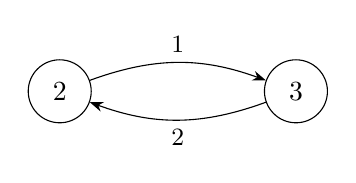
\begin{tikzpicture}[>=Stealth,
  v/.style={circle,draw,minimum size=8mm,inner sep=0pt}]
\node[v] (two) at (0,0) {$2$};
\node[v] (three) at (3,0) {$3$};
\draw[->,bend left=20] (two) to node[above]{\small 1} (three);
\draw[->,bend left=20] (three) to node[below]{\small 2} (two);
\end{tikzpicture}
\end{center}
For $28=2^2\cdot7$: $\sigma(4)=7$ and $\sigma(7)=2^3$, giving the edges
$2\xrightarrow{1}7$ and $7\xrightarrow{3}2$.
\end{example}

\begin{example}[Even perfect numbers]\label{ex:even}
For $N=2^{p-1}M_p$ the local divisor sums are $\sigma(2^{p-1})=M_p$ and
$\sigma(M_p)=2^p$.  The $\sigma$-graph is the $2$-cycle
$2\xrightarrow{1}M_p\xrightarrow{p}2$.  The in-degrees are $p$ at $2$ and $1$
at $M_p$.
\end{example}

\begin{example}[A deficient number: $15$]\label{ex:general15}
For $15=3\cdot5$: $\sigma(3)=2^2$ and $\sigma(5)=2\cdot3$.  The extended graph
on $\{2,3,5\}$ has edges $3\xrightarrow{2}2$, $5\xrightarrow{1}2$ and
$5\xrightarrow{1}3$.  The vertex $2$ is a boundary vertex.  The internal
graph on $\{3,5\}$ keeps only $5\to3$, so it is not strongly connected.  In
the figure the boundary vertex is drawn dashed, and the internal graph is
shaded.
\begin{center}
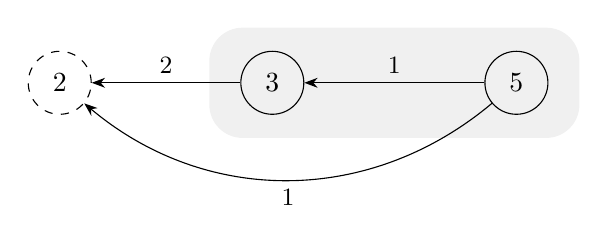
\begin{tikzpicture}[>=Stealth,
  v/.style={circle,draw,minimum size=8mm,inner sep=0pt},
  bv/.style={circle,draw,dashed,minimum size=8mm,inner sep=0pt}]
\fill[gray!12,rounded corners=12pt] (1.9,-0.7) rectangle (6.6,0.7);
\node[bv] (two) at (0,0) {$2$};
\node[v] (three) at (2.7,0) {$3$};
\node[v] (five) at (5.8,0) {$5$};
\draw[->] (three) to node[above]{\small 2} (two);
\draw[->] (five) to node[above]{\small 1} (three);
\draw[->,bend left=40] (five) to node[below]{\small 1} (two);
\end{tikzpicture}
\end{center}
\end{example}

\begin{example}[An abundant number: $12$]
For $12=2^2\cdot3$: $\sigma(4)=7$ and $\sigma(3)=2^2$.  The extended graph on
$\{2,3,7\}$ has edges $2\xrightarrow{1}7$ and $3\xrightarrow{2}2$, and $7$
is a boundary vertex:
\begin{center}
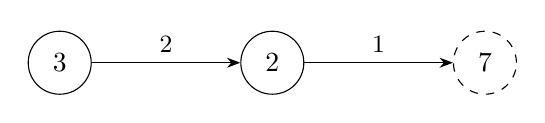
\begin{tikzpicture}[>=Stealth,
  v/.style={circle,draw,minimum size=8mm,inner sep=0pt},
  bv/.style={circle,draw,dashed,minimum size=8mm,inner sep=0pt}]
\node[v] (three) at (0,0) {$3$};
\node[v] (two) at (2.7,0) {$2$};
\node[bv] (seven) at (5.4,0) {$7$};
\draw[->] (three) to node[above]{\small 2} (two);
\draw[->] (two) to node[above]{\small 1} (seven);
\end{tikzpicture}
\end{center}
Nothing returns to $3$, which is why $d_3(12)=-1$ in
Example~\ref{ex:defects}.
\end{example}

\begin{example}[The smallest odd abundant number: $945$]\label{ex:945}
For $945=3^3\cdot5\cdot7$,
\[
\sigma(3^3)=40=2^3\cdot5,\qquad \sigma(5)=6=2\cdot3,\qquad
\sigma(7)=8=2^3 .
\]
The extended graph on $\{2,3,5,7\}$ has edges $3\xrightarrow{3}2$,
$3\xrightarrow{1}5$, $5\xrightarrow{1}2$, $5\xrightarrow{1}3$ and
$7\xrightarrow{3}2$:
\begin{center}
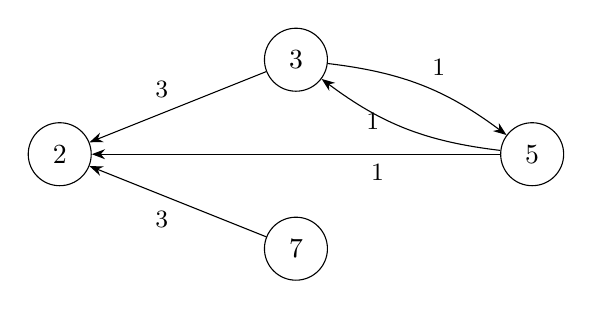
\begin{tikzpicture}[>=Stealth,
  v/.style={circle,draw,minimum size=8mm,inner sep=0pt}]
\node[v] (two) at (0,0) {$2$};
\node[v] (three) at (3,1.2) {$3$};
\node[v] (five) at (6,0) {$5$};
\node[v] (seven) at (3,-1.2) {$7$};
\draw[->] (three) to node[above left]{\small 3} (two);
\draw[->] (seven) to node[below left]{\small 3} (two);
\draw[->,bend left=15] (three) to node[above right]{\small 1} (five);
\draw[->,bend left=15] (five) to node[left,pos=0.6]{\small 1} (three);
\draw[->] (five) to node[below,pos=0.3]{\small 1} (two);
\end{tikzpicture}
\end{center}
\end{example}

\begin{example}[A $3$-perfect number: $120$]\label{ex:120}
For $120=2^3\cdot3\cdot5$, $\sigma(120)=360=3\cdot120$, and
\[
\sigma(2^3)=15=3\cdot5,\qquad\sigma(3)=4=2^2,\qquad\sigma(5)=6=2\cdot3.
\]
\begin{center}
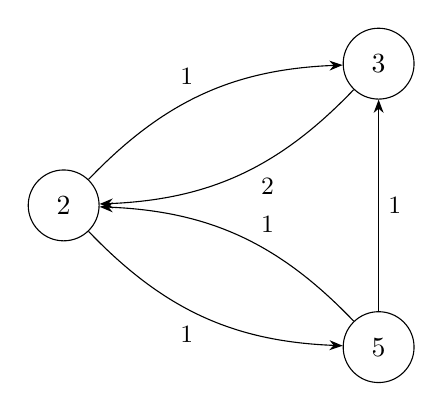
\begin{tikzpicture}[>=Stealth,
  v/.style={circle,draw,minimum size=9mm,inner sep=0pt}]
\node[v] (two) at (0,0) {$2$};
\node[v] (three) at (4,1.8) {$3$};
\node[v] (five) at (4,-1.8) {$5$};
\draw[->,bend left=22] (two) to node[above left]{\small 1} (three);
\draw[->,bend left=22] (three) to node[below right,pos=0.45]{\small 2} (two);
\draw[->,bend right=22] (two) to node[below left]{\small 1} (five);
\draw[->,bend right=22] (five) to node[above right,pos=0.45]{\small 1} (two);
\draw[->] (five) to node[right]{\small 1} (three);
\end{tikzpicture}
\end{center}
In-degrees: $2$ receives $2+1=3$, $3$ receives $1+1=2$, and $5$ receives
$1$.  Here every prime of $\sigma(120)$ divides $120$, so there are no
boundary vertices.
\end{example}

\subsection{The defect vector and the Poisson equation}\label{sec:poissongeneral}

Write $b_r=\sum_s w(s,r)$ for the in-degree of $r$ in
$\widehat G_\sigma(n)$.  Since $\sigma(n)$ is the product of the local
divisor sums,
\[
b_r=v_r\bigl(\sigma(n)\bigr)\qquad(r\in\widehat S(n)).
\]
Comparing with $a_r=v_r(n)$ gives the basic identity.

\begin{proposition}[Valuation defect]\label{prop:defect}
Define the \emph{defect vector} $d(n)=(b_r-a_r)_{r\in\widehat S(n)}$.  Then
\[
h(n)=\frac{\sigma(n)}{n}=\prod_{r\in\widehat S(n)}r^{\,d_r(n)} .
\]
Consequently $n$ is $k$-perfect if and only if $d_r(n)=v_r(k)$ for every $r$.
In particular $n$ is multiperfect exactly when $d(n)\ge0$, and perfect
exactly when $d(n)$ is the unit vector $e_2$ at the prime $2$.
\end{proposition}

\begin{proof}
$h(n)=\prod_r r^{v_r(\sigma(n))-v_r(n)}=\prod_r r^{b_r-a_r}$.  A positive
rational is determined by its valuations.
\end{proof}

\begin{example}[Defect vectors]\label{ex:defects}
\begin{center}
\begin{tabular}{@{}lllll@{}}
\toprule
$n$ & vertices & in-degrees $b$ & exponents $a$ & defect $d(n)$\\
\midrule
$6$ & $2,3$ & $(2,1)$ & $(1,1)$ & $(1,0)=e_2$\\
$28$ & $2,7$ & $(3,1)$ & $(2,1)$ & $(1,0)=e_2$\\
$15$ & $2,3,5$ & $(3,1,0)$ & $(0,1,1)$ & $(3,0,-1)$\\
$12$ & $2,3,7$ & $(2,0,1)$ & $(2,1,0)$ & $(0,-1,1)$\\
$945$ & $2,3,5,7$ & $(7,1,1,0)$ & $(0,3,1,1)$ & $(7,-2,0,-1)$\\
$120$ & $2,3,5$ & $(3,2,1)$ & $(3,1,1)$ & $(0,1,0)=e_3$\\
\bottomrule
\end{tabular}
\end{center}
Each row reproduces $h(n)$.  For instance $h(15)=2^3\cdot5^{-1}=8/5$, and
$h(945)=2^7\cdot3^{-2}\cdot7^{-1}=128/63$.  The odd abundant number $945$
overshoots $2$, but its defect is far from $e_2$: the boundary vertex $2$
receives weight $7$, because all three local divisor sums are even.
\end{example}

The defect has a linear-algebra meaning.  Let $W$ be the weight matrix of
$\widehat G_\sigma(n)$, put $D=\operatorname{diag}(a_s)$ and $L=D-W$.  Let
$\ell=(\log s)_{s}$ be the \emph{log-prime vector}, and let
$\eta_s=\log h(s^{a_s})$ be the logarithmic local abundancy (so $\eta_s=0$ at
a boundary vertex).

\begin{proposition}[The Poisson equation of an integer]\label{prop:poisson}
For every integer $n>1$,
\[
L\ell=-\eta,\qquad \one^{\mathsf T}L=-d(n)^{\mathsf T},\qquad
\sum_s\eta_s=\log h(n).
\]
\end{proposition}

\begin{proof}
Row $s$ of $L\ell$ is
$a_s\log s-\sum_r w(s,r)\log r=a_s\log s-\log\sigma(s^{a_s})=-\eta_s$.
Column $r$ of $L$ sums to $a_r-b_r=-d_r(n)$.  Finally
$\sum_s\eta_s=\log\prod_s h(s^{a_s})=\log h(n)$ by
Lemma~\ref{lem:abundancy}(a).
\end{proof}

So $\ell$ is a \emph{potential} whose ``Laplacian'' is the vector of local
log-abundancies, and the defect measures how far $L$ is from being an
in-degree Laplacian.  For a $k$-perfect number, $\one^{\mathsf T}L=-v(k)^{\mathsf T}$.

\begin{example}[$n=6$]
In the order $(2,3)$, $D=\operatorname{diag}(1,1)$ and
\[
L=\begin{pmatrix}1&-1\\-2&1\end{pmatrix},\qquad
L\ell=\begin{pmatrix}\log\frac23\\[2pt]\log\frac34\end{pmatrix}
=-\begin{pmatrix}\log h(2)\\ \log h(3)\end{pmatrix}.
\]
The column sums are $(-1,0)=-e_2$, and $\eta_2+\eta_3=\log(\tfrac32\cdot\tfrac43)=\log2$.
\end{example}

\begin{example}[$n=120$]\label{ex:120poisson}
In the order $(2,3,5)$,
\[
L=\begin{pmatrix}3&-1&-1\\-2&1&0\\-1&-1&1\end{pmatrix},\qquad
L\ell=\begin{pmatrix}\log\frac{8}{15}\\[2pt]\log\frac34\\[2pt]\log\frac56\end{pmatrix}
=-\begin{pmatrix}\log h(2^3)\\ \log h(3)\\ \log h(5)\end{pmatrix}.
\]
The column sums are $(0,-1,0)=-e_3$, and
$\sum\eta_s=\log\bigl(\tfrac{15}{8}\cdot\tfrac43\cdot\tfrac65\bigr)=\log3$.
\end{example}

\begin{remark}[Taking logarithms loses nothing]\label{rem:logs}
The numbers $\log r$, $r$ prime, are linearly independent over $\mathbb Q$:
if $\sum_r c_r\log r=0$ with rational $c_r$, clear denominators and
exponentiate to get $\prod_r r^{mc_r}=1$, so every $c_r=0$.  Passing from a
multiplicative identity among prime powers to its logarithm is therefore
injective as long as the coefficients stay rational.  Information is lost
only when the coefficients are relaxed to arbitrary reals, or when several
primes are merged into one composite coordinate.
\end{remark}

\subsection{Harmonic morphisms and equitable partitions}\label{sec:hm}

\begin{definition}[Harmonic morphisms]
A morphism $\varphi\colon G\to H$ of undirected multigraphs is
\emph{harmonic} if for every vertex $x$ of $G$ the number
\[
m_\varphi(x)=\#\{e\ni x:\ \varphi(e)=e'\}
\]
is the same for every edge $e'$ of $H$ at $\varphi(x)$.  Edges that map to
vertices are \emph{vertical}.
\end{definition}

See Urakawa~\cite{Urakawa}, Baker--Norine~\cite{BN},
Joyner--Melles~\cite{JM2017}, and, for the weighted theory, the chapter
``Weighted harmonic morphisms'' of~\cite{MJappl}.  With
$\Delta f(x)=\sum_{e=xy}(f(x)-f(y))$, the basic identity is
\[
\Delta_G(f\circ\varphi)(x)=m_\varphi(x)\,(\Delta_H f)(\varphi(x)),
\tag{B2}
\]
because vertical edges contribute $0$ and each edge $e'$ at $\varphi(x)$ is
covered exactly $m_\varphi(x)$ times.  Baker and Norine also show that
pullback and pushforward of divisors preserve principal divisors.

For a weighted digraph, a vertex quotient is given by a partition
$V=C_1\sqcup\cdots\sqcup C_k$.  The harmonic condition becomes an
equitability condition, and for a digraph there are two of them.

\begin{definition}[Equitable partitions of a digraph]
A partition of $V$ is
\begin{itemize}[leftmargin=1.5em]
\item \emph{in-equitable} if for all cells $C,C'$ the in-weight
  $\sum_{s\in C}w(s,r)$ is the same number $b_{CC'}$ for every $r\in C'$;
\item \emph{out-equitable} if for all cells $C,C'$ the out-weight
  $\sum_{r\in C'}w(s,r)$ is the same number $b'_{CC'}$ for every $s\in C$.
\end{itemize}
The matrices $(b_{CC'})$ and $(b'_{CC'})$ are the corresponding quotient
matrices.
\end{definition}

For a symmetric $W$ the two notions coincide with the weighted equitable
partitions of the chapter ``Edge-weighted graph partitions''
of~\cite{MJappl}: each vertex of a cell sends the same total weight to each
cell.  In matrix terms, an out-equitable partition is one whose cell
indicator vectors span a $W$-invariant subspace; an in-equitable partition
does the same for $W^{\mathsf T}$.

\begin{example}[Equitability is rare]
In the $\sigma$-graph of $120$ (Example~\ref{ex:120}), try the partition
$\{2\},\{3,5\}$.  The in-weight from $\{3,5\}$ into $3$ is
$w(3,3)+w(5,3)=1$, but into $5$ it is $w(3,5)+w(5,5)=0$.  So the partition is
not in-equitable.  The out-weight from $3$ into $\{2\}$ is $2$, but from $5$
it is $1$, so it is not out-equitable either.
\end{example}

\subsection{Arithmetical structures}\label{sec:arithdefs}

\begin{definition}[Lorenzini]\label{def:arith}
Let $\Gamma=(V,E)$ be a connected (multi)graph with adjacency matrix $A$.  An
\emph{arithmetical structure} on $\Gamma$ is a pair of maps
$R,S\colon V\to\mathbb Z_{>0}$ such that $\gcd\{R(v):v\in V\}=1$ and
\[
R(v)\,S(v)=\sum_{w\sim v}R(w)\qquad(v\in V),
\]
the sum counting multiple edges with multiplicity.  Equivalently,
$(\operatorname{diag}(S)-A)R=0$.  The matrix
$\operatorname{diag}(S)-A$ is the \emph{generalized Laplacian} of the
structure, and the torsion subgroup of its cokernel
$\mathbb Z^V/(\operatorname{diag}(S)-A)\mathbb Z^V$ is the
\emph{arithmetical critical group} $K(\Gamma;R,S)$.
\end{definition}

Arithmetical structures are due to Lorenzini~\cite{Lorenzini}.  Every
connected graph has the \emph{natural} structure $R\equiv1$, $S=\deg$, whose
generalized Laplacian is the ordinary Laplacian and whose critical group is
the usual critical (sandpile) group.  Other structures exist as well;
\cite{MJappl} gives the example $R=(1,1,2)$, $S=(3,3,1)$ on the triangle
$C_3$.  That source also shows that a harmonic morphism
$\phi\colon\Gamma_2\to\Gamma_1$ pulls an arithmetical structure $(R_1,S_1)$
back to $(R_1\circ\phi,\ \mu S_1\circ\phi+\nu)$, where $\mu$ and $\nu$ are
the horizontal and vertical multiplicities, and that the generalized
Laplacians then satisfy $Q_2\Phi=D_\mu\Phi Q_1$.

Nothing in Definition~\ref{def:arith} uses the symmetry of $A$.  So it
extends verbatim to weighted digraphs, in two ways.

\begin{definition}[Arithmetical structures on a weighted digraph]
Let $W$ be the weight matrix of a strongly connected digraph on $V$.  A pair
$(R,S)$ of positive integer vectors with $\gcd R=1$ is
\begin{itemize}[leftmargin=1.5em]
\item an \emph{out-structure} if $S(s)R(s)=\sum_r w(s,r)R(r)$ for all $s$,
  i.e.\ $(\operatorname{diag}(S)-W)R=0$;
\item an \emph{in-structure} if $S(r)R(r)=\sum_s w(s,r)R(s)$ for all $r$,
  i.e.\ $R^{\mathsf T}(\operatorname{diag}(S)-W)=0$.
\end{itemize}
In both cases $\operatorname{diag}(S)-W$ is the generalized Laplacian, and
the arithmetical critical group is the torsion of its cokernel.  For a
symmetric $W$ both notions agree with Definition~\ref{def:arith}.
\end{definition}

An in-structure on $G$ is an out-structure on the reversed digraph.  The
pair $(\one,\text{in-degrees})$ is always an in-structure, the directed
analogue of the natural structure.  When $S$ is the vector of in-degrees,
the out-degree Laplacian of the reversed digraph is
$Q'=\operatorname{diag}(S)-W^{\mathsf T}$, and the vector $R$ of an
out-structure is exactly the positive vector with $Q'^{\mathsf T}R=0$.  For
strongly connected digraphs this vector is central to Asadi--Backman's
chip-firing and Riemann--Roch theory for directed graphs~\cite{AsadiBackman}.

\begin{example}[The $2$-cycle of $6$]
For the digraph of Example~\ref{ex:twocycle}, take $S$ to be the in-degrees
$(2,1)$.  The out-structure equations are $2R(2)=R(3)$ and $R(3)=2R(2)$, so
$R=(1,2)$.  The in-structure with the same $S$ is $R=(1,1)$.  The two
structures share the generalized Laplacian
$\begin{pmatrix}2&-1\\-2&1\end{pmatrix}$, with right kernel spanned by
$(1,2)$ and left kernel by $(1,1)$.
\end{example}

\subsection{Undirected encodings of a digraph}\label{sec:encodings}

A digraph can be turned into an undirected graph in several ways.  Some keep
all the information; some do not.

\begin{definition}
Let $G$ be a weighted digraph on $V$ with weight matrix $W$.
\begin{itemize}[leftmargin=1.5em]
\item The \emph{underlying graph} $U(G)$ is the simple graph with an edge
  $\{s,r\}$ whenever $w(s,r)>0$ or $w(r,s)>0$.
\item The \emph{source--target bipartite graph} $B(G)$ has two copies
  $V^-=\{s^-\}$ and $V^+=\{r^+\}$ of $V$, and an undirected edge
  $s^-\!-\!r^+$ of weight $w(s,r)$.  Its biadjacency matrix is $W$.
\item The \emph{symmetric dilation} of $W$ is
  $\begin{pmatrix}0&W\\W^{\mathsf T}&0\end{pmatrix}$, the weighted
  adjacency matrix of $B(G)$.
\end{itemize}
$G$ is \emph{symmetric} if $W=W^{\mathsf T}$.  Then $G$ is just an
undirected multigraph with $w(s,r)$ parallel edges between $s$ and $r$.
\end{definition}

$B(G)$ loses nothing, provided its two color classes and labels are kept:
the weighted degree of $r^+$ is the in-degree of $r$, and that of $s^-$ is
the out-degree of $s$.  This correspondence between digraphs and balanced
bipartite graphs is classical; see
Brualdi--Harary--Miller~\cite{BrualdiHararyMiller}.  The nonzero eigenvalues
of the symmetric dilation are $\pm$ the singular values of $W$.  By contrast
$U(G)$ forgets both direction and weight.

Two facts about undirected graphs will be used for symmetric $\sigma$-graphs.
\begin{itemize}[leftmargin=1.5em]
\item \textbf{Handshake lemma.}  The degrees of an undirected multigraph sum
  to twice the number of edges.  So the number of odd-degree vertices is
  even.
\item \textbf{Maximum principle.}  For a Laplacian
  $\Delta f(x)=\sum_y w(x,y)(f(x)-f(y))$ with $w\ge0$, at a vertex where $f$
  is largest $\Delta f\ge0$, with strict inequality if some neighbor has a
  smaller value.
\end{itemize}

\begin{example}
For the $\sigma$-graph of $6$, $U(G)$ is a single edge $\{2,3\}$.  The graph
$B(G)$ has edges $2^-\!-\!3^+$ of weight $1$ and $3^-\!-\!2^+$ of weight
$2$.  The degree of $2^+$ is $2$, the in-degree of $2$.  The $\sigma$-graph of
$6$ is not symmetric, since $w(2,3)=1\ne2=w(3,2)$.
\end{example}

\subsection{Divisor graphs and Hasse graphs}\label{sec:divisorgraphs}

The $\sigma$-graph has \emph{primes} as vertices.  A more classical graph
uses \emph{divisors} as vertices.  Divisor graphs have a literature of their
own, surveyed by Ravi and Desikan~\cite{RaviDesikan}.

\begin{definition}
Let $n=\prod_{i=1}^k p_i^{a_i}>1$.
\begin{itemize}[leftmargin=1.5em]
\item The \emph{divisor lattice} $\operatorname{Div}(n)$ is the set of
  positive divisors of $n$, partially ordered by divisibility.  It is a
  lattice in the order-theoretic sense, with meet $\gcd$ and join
  $\operatorname{lcm}$.  Its bottom element is $1$ and its top element is $n$.
\item The \emph{divisor graph} $D(n)$ is the comparability graph of
  $\operatorname{Div}(n)$: its vertices are the divisors, with distinct
  $d,d'$ adjacent when $d\mid d'$ or $d'\mid d$.
\item The \emph{Hasse graph} $H(n)$ is the undirected graph of covering
  relations of $\operatorname{Div}(n)$: $d$ and $d'$ are adjacent when
  $d'=dp$ for a prime $p$.  Coloring such an edge by $p$ gives an
  edge-colored graph.
\end{itemize}
\end{definition}

\paragraph{Terminology.}
These notes keep three objects apart.
\begin{itemize}[leftmargin=1.5em]
\item ``Divisor lattice'' always means the poset $\operatorname{Div}(n)$.
\item ``Hasse graph'' means the undirected graph $H(n)$.
\item ``Labeled Hasse graph'' means $H(n)$ together with the vertex weights
  $m(d)=d$.
\end{itemize}
As an unlabeled graph, $H(n)$ does not know which corner is $1$ and which is
$n$, since reversing a path is a graph automorphism.  The labels, or
equivalently the order of $\operatorname{Div}(n)$, single out the bottom
vertex $1$ and the top vertex $n$.  Words such as ``top'' and ``upward''
always refer to the divisibility order.

Writing a divisor as an exponent vector $(e_1,\dots,e_k)$ with
$0\le e_i\le a_i$ identifies $H(n)$ with a Cartesian product of paths,
\[
H(n)\cong P_{a_1+1}\,\square\,P_{a_2+1}\,\square\cdots\square\,P_{a_k+1},
\]
in which the edges of color $p_i$ are those in the $i$th coordinate
direction.

\begin{example}[$D(6)$, $H(6)$ and $H(28)$]\label{ex:divisor28}
The divisors of $6$ are $1,2,3,6$.  Every pair is comparable except
$\{2,3\}$, so $D(6)$ is $K_4$ with one edge removed, and $H(6)$ is the
$4$-cycle $1-2-6-3-1\cong P_2\,\square\,P_2$.  For $28=2^2\cdot7$, the
graph $H(28)\cong P_3\,\square\,P_2$ is a $2\times3$ grid.  Horizontal edges
have color $2$ and vertical edges color $7$:
\begin{center}
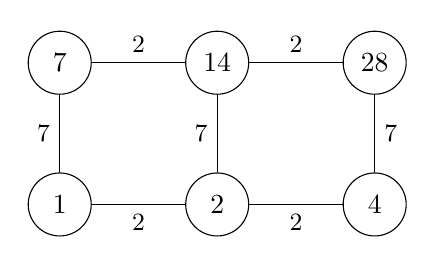
\begin{tikzpicture}[
  v/.style={circle,draw,minimum size=8mm,inner sep=0pt}]
\node[v] (a) at (0,0) {$1$};
\node[v] (b) at (2,0) {$2$};
\node[v] (c) at (4,0) {$4$};
\node[v] (d) at (0,1.8) {$7$};
\node[v] (e) at (2,1.8) {$14$};
\node[v] (f) at (4,1.8) {$28$};
\draw (a)--node[below]{\small 2}(b)--node[below]{\small 2}(c);
\draw (d)--node[above]{\small 2}(e)--node[above]{\small 2}(f);
\draw (a)--node[left]{\small 7}(d);
\draw (b)--node[left]{\small 7}(e);
\draw (c)--node[right]{\small 7}(f);
\end{tikzpicture}
\end{center}
\end{example}

\paragraph{The shape depends only on the exponents.}
The divisibility order of $n$ is a product of chains whose lengths are the
exponents.  So, as unlabeled graphs, $D(n)$ and $H(n)$ depend only on the
multiset of exponents of $n$, not on its primes.

\begin{example}[One graph, three kinds of numbers]\label{ex:onegraph}
The numbers $12=2^2\cdot3$, $28=2^2\cdot7$ and $45=3^2\cdot5$ all have
exponent pattern $\{2,1\}$.  So $H(12)\cong H(28)\cong H(45)$ (the grid of
Example~\ref{ex:divisor28}), and likewise for $D$.  Yet $12$ is abundant,
$28$ is perfect, and $45$ is deficient.  Similarly
$D(6)\cong D(15)\cong D(35)$, with only $6$ perfect.
\end{example}

\begin{example}[The Hasse graph $H(945)$]\label{ex:H945}
For $945=3^3\cdot5\cdot7$ the graph $H(945)\cong P_4\,\square\,P_2\,\square\,P_2$
has $\sigma_0(945)=16$ vertices.  In the figure, solid edges multiply by $3$,
dashed edges by $5$, and dotted edges by $7$.  The back layer is the front
layer times $7$.
\begin{center}
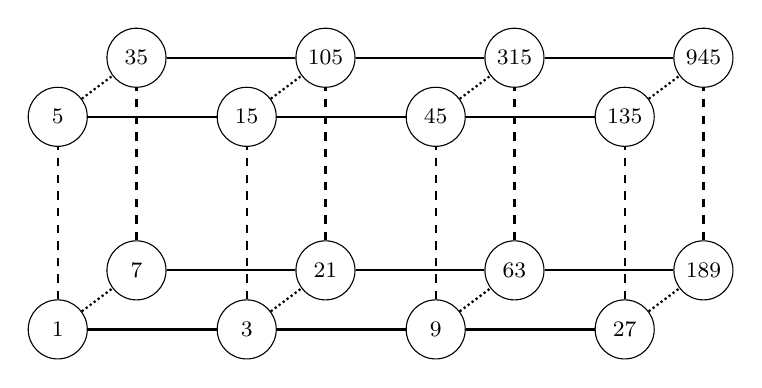
\begin{tikzpicture}[
  v/.style={circle,draw,fill=white,minimum size=7.5mm,inner sep=0pt,font=\footnotesize},
  e3/.style={thick},
  e5/.style={thick,dashed},
  e7/.style={thick,densely dotted}]
\def\dx{1.0}\def\dy{0.75}
% back layer (times 7)
\foreach \i/\a/\b in {0/7/35,1/21/105,2/63/315,3/189/945}{
  \node[v] (b\i) at ({2.4*\i+\dx},{\dy}) {$\a$};
  \node[v] (bt\i) at ({2.4*\i+\dx},{2.7+\dy}) {$\b$};
}
\foreach \i in {0,1,2}{\pgfmathtruncatemacro{\j}{\i+1}
  \draw[e3] (b\i)--(b\j); \draw[e3] (bt\i)--(bt\j);}
\foreach \i in {0,1,2,3}{\draw[e5] (b\i)--(bt\i);}
% front layer
\foreach \i/\a/\b in {0/1/5,1/3/15,2/9/45,3/27/135}{
  \node[v] (f\i) at ({2.4*\i},0) {$\a$};
  \node[v] (ft\i) at ({2.4*\i},2.7) {$\b$};
}
\foreach \i in {0,1,2,3}{\draw[e7] (f\i)--(b\i); \draw[e7] (ft\i)--(bt\i);}
\foreach \i in {0,1,2}{\pgfmathtruncatemacro{\j}{\i+1}
  \draw[e3] (f\i)--(f\j); \draw[e3] (ft\i)--(ft\j);}
\foreach \i in {0,1,2,3}{\draw[e5] (f\i)--(ft\i);}
\end{tikzpicture}
\end{center}
The vertex labels add up to $\sigma(945)=40\cdot6\cdot8=1920$, and the
three coordinate chains have sums $40$, $6$ and $8$.  These are the local
divisor sums whose factorizations give the $\sigma$-graph of
Example~\ref{ex:945}.
\end{example}

\begin{remark}[A terminology trap]
In graph theory a \emph{perfect graph} is one in which every induced
subgraph has chromatic number equal to its clique number.  This has nothing
to do with perfect numbers.  In fact every divisor graph $D(n)$ is a perfect
graph, because comparability graphs of partial orders are perfect.
\end{remark}

\paragraph{The labeled Hasse graph and its partition function.}
Give the vertex $(e_1,\dots,e_k)$ of $H(n)$ the weight
$m(e)=\prod_ip_i^{e_i}$, the divisor it represents, and put
$Z(n)=\sum_v m(v)$.  Because $H(n)$ is a product of paths, $Z$ factors:
\[
Z(n)=\prod_{i=1}^k\bigl(1+p_i+\cdots+p_i^{a_i}\bigr)=\prod_{i=1}^k\sigma(p_i^{a_i})=\sigma(n).
\]
For the grid of Example~\ref{ex:divisor28}, $Z(28)=(1+2+4)(1+7)=56$.

\paragraph{Harmonic projections.}
The coordinate projection $\pi_i\colon H(n)\to P_{a_i+1}$,
$(e_1,\dots,e_k)\mapsto e_i$, is a harmonic morphism.  Each edge of the path
at $e_i$ has exactly one edge above it at every vertex of the fiber, so the
horizontal multiplicity is $1$; the edges in the other directions are
vertical.  Pushing $m$ forward along $\pi_i$ gives
\[
(\pi_i)_*m\,(e)=p_i^{\,e}\prod_{j\ne i}\sigma\bigl(p_j^{a_j}\bigr).
\]
So the partition function of the labeled Hasse graph is assembled from the
partition functions $\sigma(p_i^{a_i})$ of its coordinate paths.  In
$\operatorname{Div}(n)$ these paths are the chains $1,p_i,\dots,p_i^{a_i}$,
so $\sigma(p_i^{a_i})$ is called the $i$th \emph{chain sum}.

\paragraph{An edge-weighted version.}
The vertex labels of $H(n)$ can be traded for edge weights.  Give the edge
from $d$ to $dp$ the weight $1/p$.  Along any upward path from $d$ to $n$,
the product of the edge weights is $d/n$, whatever path is chosen.  (Around
each square $d,dp,dq,dpq$ the two routes give the same product, and these
squares generate the cycle space.)  So the vertex labels are recovered from
the edge weights, and
\[
h(n)=\sum_{d\mid n}\frac dn=\sum_{v}\ \prod_{e\in\text{path}(v\to n)}w(e).
\]
In additive form, with edge length $\log p$ the distance from $d$ to $n$ is
$\log(n/d)$, and $h(n)=\sum_v e^{-\operatorname{dist}(v,n)}$.  This is an
exact duality between vertex weights and edge weights.  It adds no
arithmetic information: the edge weights are a gradient of the vertex
potential $\log d$.

\begin{example}[Edge weights on $H(12)$]\label{ex:H12edges}
For $12=2^2\cdot3$, horizontal edges multiply by $2$ and get weight
$\tfrac12$; vertical edges multiply by $3$ and get weight $\tfrac13$:
\begin{center}
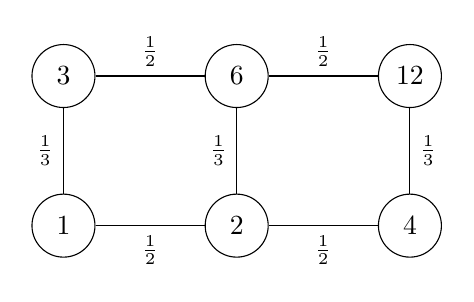
\begin{tikzpicture}[
  v/.style={circle,draw,minimum size=8mm,inner sep=0pt}]
\node[v] (a) at (0,0) {$1$};
\node[v] (b) at (2.2,0) {$2$};
\node[v] (c) at (4.4,0) {$4$};
\node[v] (d) at (0,1.9) {$3$};
\node[v] (e) at (2.2,1.9) {$6$};
\node[v] (f) at (4.4,1.9) {$12$};
\draw (a)--node[below]{\small $\frac12$}(b)--node[below]{\small $\frac12$}(c);
\draw (d)--node[above]{\small $\frac12$}(e)--node[above]{\small $\frac12$}(f);
\draw (a)--node[left]{\small $\frac13$}(d);
\draw (b)--node[left]{\small $\frac13$}(e);
\draw (c)--node[right]{\small $\frac13$}(f);
\end{tikzpicture}
\end{center}
From $2$ up to $12$ the weights multiply to $\tfrac12\cdot\tfrac13=\tfrac16=\tfrac2{12}$,
by either route.  Summing over all six vertices gives
$1+\tfrac12+\tfrac13+\tfrac14+\tfrac16+\tfrac1{12}=\tfrac73=h(12)$.
\end{example}

\paragraph{How the Hasse graph and the $\sigma$-graph fit together.}
The chain sums $\sigma(p_i^{a_i})$ are exactly the local divisor sums from
which the $\sigma$-graph is built.  The out-edges of $p_i$ in
$\widehat G_\sigma(n)$ record the prime factorization of the $i$th chain
sum.  So the two graphs play complementary roles.
\begin{itemize}[leftmargin=1.5em]
\item The labeled Hasse graph $H(n)$ records the \emph{product structure}:
  $\sigma(n)$ is a product of chain sums.
\item The $\sigma$-graph records the \emph{interaction}: which primes occur
  in which chain sums, and how often.
\end{itemize}

\begin{example}[$28$ in both languages]\label{ex:28both}
In $H(28)$ the chain in the $2$-direction has sum $1+2+4=7$, and the chain
in the $7$-direction has sum $1+7=8=2^3$.  In $\widehat G_\sigma(28)$ these
become the edges $2\xrightarrow{1}7$ and $7\xrightarrow{3}2$.  Multiplying,
$7\cdot2^3=2\cdot28$: the prime $7$ returns once, matching its exponent
$1$, and the prime $2$ returns three times, one more than its exponent $2$.
That extra factor of $2$ is the defect $d(28)=e_2$.
\end{example}

%=====================================================================
\section{Odd perfect numbers and their $\sigma$-graphs}\label{sec:opn}
%=====================================================================

From now on $N$ denotes a hypothetical odd perfect number, so
$\sigma(N)=2N$.  This section specializes the general constructions to $N$.

\subsection{Euler's form and the vertex data}\label{sec:notation}

Euler showed that an OPN has the form
\[
N=p^{\alpha}\prod_{q\in Q}q^{2\beta_q},\qquad
p\equiv\alpha\equiv 1\pmod 4,
\]
with $p\notin Q$ and all primes odd.  The prime $p$ is the \emph{Euler} (or
special) prime, and every $q\in Q$ is \emph{nonspecial}.  Correspondingly
$p^\alpha$ is the \emph{special component} and the $q^{2\beta_q}$ are the
\emph{nonspecial components}.

\begin{definition}[Vertex data]
Put $S=\{p\}\cup Q$, the set of prime divisors of $N$.  For $s\in S$ let
\[
a_s=\begin{cases}\alpha,&s=p,\\ 2\beta_s,&s\in Q,\end{cases}
\qquad\qquad n_s=a_s+1 .
\]
Thus $n_q$ is odd for $q\in Q$, while $n_p=\alpha+1\equiv 2\pmod 4$.  For
nonspecial $q$ we also write $e_q=n_q=2\beta_q+1$.
\end{definition}

Note that $\omega(N)=|S|$ and $\Omega(N)=\sum_{s\in S}a_s$.

\paragraph{Local divisor sums.}
For each $s\in S$, $\sigma(s^{a_s})=(s^{n_s}-1)/(s-1)$, and
$\sigma(N)=\prod_{s\in S}\sigma(s^{a_s})$.  The congruences in Euler's form
give $v_2(\sigma(p^\alpha))=1$, while each $\sigma(q^{2\beta_q})$ is odd.  So
we define the \emph{odd local divisor sum}
\[
\Sigma_s=\begin{cases}\sigma(p^\alpha)/2,&s=p,\\ \sigma(q^{a_q}),&s=q\in Q,\end{cases}
\qquad\text{so that}\qquad \prod_{s\in S}\Sigma_s=N .
\]

\begin{definition}[Exponent excess]
$E(N)=\Omega(N)-(2\omega(N)-1)=(\alpha-1)+\sum_{q\in Q}(2\beta_q-2)$.
It vanishes exactly when $\alpha=1$ and every $\beta_q=1$.
\end{definition}

\subsection{The $\sigma$-graph $G_N$}\label{sec:GN}

The extended $\sigma$-graph of an OPN has exactly one boundary vertex, the
prime $2$.  It receives a single edge, of weight $1$, from the Euler prime.
Deleting it gives the graph used throughout the rest of these notes.

\begin{definition}[The $\sigma$-graph of an OPN]
The \emph{$\sigma$-graph} $G_N$ is the weighted digraph on $S$ with
\[
w(s,r)=v_r\bigl(\Sigma_s\bigr)=v_r\bigl(\sigma(s^{a_s})\bigr)\qquad(s,r\in S).
\]
Write $W=(w(s,r))_{s,r\in S}$ and $D=\operatorname{diag}(a_s)$.
\end{definition}

So $G_N$ is the internal $\sigma$-graph of $N$, and also the extended
$\sigma$-graph with the vertex $2$ removed.  For odd $r$ the factor $2$ in
$\Sigma_p$ is irrelevant.  Every weight is computed by
Proposition~\ref{prop:edgeweights}.

\begin{definition}[Logarithmic quantities]
Let $\ell\in\R^S$ be the log-prime vector, $\ell_s=\log s$.  Define
\[
\delta_s=\log\Sigma_s-a_s\log s,
\]
the logarithm of the odd local abundancy.  For $A,B\subseteq S$ define the
\emph{logarithmic flow}
\[
L(A,B)=\sum_{s\in A}\sum_{r\in B}w(s,r)\log r .
\]
\end{definition}

For $q\in Q$, $\delta_q=\eta_q=\log h(q^{a_q})$.  For the Euler prime,
$\delta_p=\eta_p-\log2$, which accounts for the deleted vertex $2$.

\begin{definition}[Cyclotomic obligations]
For $q\in Q$ and $d\mid e_q$ with $d>1$, the pair $(q,d)$ is a
\emph{cyclotomic obligation}.  Its set of possible targets is
\[
P(q,d)=\{r\in S:\ \ord_r(q)=d\}.
\]
Write $\mathcal O$ for the set of all obligations.
\end{definition}

By Proposition~\ref{prop:layers}, the obligations at $q$ are the cyclotomic
layers of $\sigma(q^{a_q})$; there are $\sigma_0(e_q)-1$ of them.

\begin{definition}[Edge terminology]
Let $q\in Q$ and suppose $q\to r$.  The edge is an \emph{order-one edge}
if $\ord_r(q)=1$.  If $d=\ord_r(q)>1$, it is an \emph{order-$d$ edge};
equivalently, $r$ is a primitive prime divisor of $q^d-1$.  When the
obligation in question is $(q,d)$, such an edge is also called a
\emph{primitive edge of level $d$}.  A \emph{multiplier contribution} is not
a separate edge type: it is the extra valuation $v_r(n_q/d)$ that can sit on
an order-$d$ edge when $r\mid n_q/d$.
\end{definition}

\subsection{Defect and Poisson forms of the OPN conjecture}\label{sec:poisson}

Proposition~\ref{prop:defect} gives the first reformulation at once.

\begin{corollary}[Defect form of the OPN conjecture]\label{cor:defect}
There is an odd perfect number if and only if there is an odd $n>1$ whose
extended $\sigma$-graph has defect vector $e_2$.  That is, the boundary
vertex $2$ receives total weight exactly $1$, and every other vertex receives
total weight exactly equal to its exponent.
\end{corollary}

For odd $n$ the vertex $2$ is always a boundary vertex, and
$d_2(n)=v_2(\sigma(n))$ is the total power of $2$ contributed by the local
divisor sums.  So Corollary~\ref{cor:defect} repackages two classical facts:
exactly one local divisor sum is even (this is Euler's special prime), and it
is $\equiv2\pmod 4$.  The odd abundant number $945$ fails badly: all three of
its local divisor sums are even (Example~\ref{ex:defects}).

Deleting the boundary vertex turns the general Poisson equation of
Proposition~\ref{prop:poisson} into a cleaner one.

\begin{proposition}[The Poisson equation of an OPN]\label{prop:poissonOPN}
For an odd perfect number, with $L=D-W$ on $S$,
\[
\boxed{\;L\ell=-\delta,\qquad \one^{\mathsf T}L=0\;}
\]
where $\delta_q>0$ for $q\ne p$ and $\delta_p<0$.
\end{proposition}

\begin{proof}
Row $s$ of $L\ell$ is $a_s\log s-\log\Sigma_s=-\delta_s$.  Column $r$ sums to
$a_r-v_r(N)=0$, because $\prod_s\Sigma_s=N$.  The signs come from
Lemma~\ref{lem:abundancy}(b): $\Sigma_q=\sigma(q^{a_q})>q^{a_q}$, while
$\sigma(p^\alpha)/p^\alpha<p/(p-1)\le5/4<2$.
\end{proof}

So $L$ has zero column sums: it is an in-degree Laplacian.  The log-prime
vector is a \emph{potential} for the real degree-zero vector $\delta$, which
is positive everywhere except at the Euler prime.  This is formally analogous
to a principal divisor with potential $\log$, but it is not literally the
Baker--Norine notion.  Baker--Norine theory uses undirected graphs,
integral divisors and integral firing functions; here the operator is
directed and $\ell$ is real-valued.

Two quick consequences:
\begin{itemize}[leftmargin=1.5em]
\item $\sum_s\delta_s=\one^{\mathsf T}(-L\ell)=0$.  This is the Fredholm
  compatibility condition for the left null vector $\one^{\mathsf T}$.  For
  a general directed Laplacian there may be more left null vectors.  For an
  OPN there are not: $G_N$ is strongly connected
  (Proposition~\ref{prop:strong}), so $L$ has rank $|S|-1$
  (Corollary~\ref{cor:rank}).
\item Summing the equation over a set $T$ gives the cut identity (L5) of
  Section~\ref{sec:program}.
\end{itemize}

Constant vectors need not satisfy $L\one=0$: $L\one=(a_s-\Omega(\Sigma_s))_s$.
Its entries sum to $0$, since both $\sum_s a_s$ and $\sum_s\Omega(\Sigma_s)$
equal $\Omega(N)$, but nothing forces them all to vanish.  This vector
reappears as the ``potential'' in the quadratic-form identity of
Section~\ref{sec:undirected}.

The OPN conjecture is therefore equivalent to:

\begin{quote}
\emph{There is no finite set $S$ of odd primes with Euler-form exponents
$a_s$ such that the integer matrix $W$ defined by
$w(s,r)=v_r(\Sigma_s)$ satisfies $\one^{\mathsf T}(D-W)=0$ and
$\sigma$-closure.}
\end{quote}
Given those, $L\ell=-\delta$ is automatic.

\subsection{What is general and what is forced}\label{sec:forced}

The examples of Section~\ref{sec:graphs} show which features of $G_N$ are
special to perfectness.
\begin{itemize}[leftmargin=1.5em]
\item \textbf{General.}  The order/LTE classification of edge weights
  (Proposition~\ref{prop:edgeweights}), the cyclotomic layers
  (Proposition~\ref{prop:layers}), primitive prime divisors
  (Theorem~\ref{thm:zsigmondy}), and the identities
  $b_r=v_r(\sigma(n))$ and $L\ell=-\eta$ hold for every integer.
\item \textbf{Forced by perfectness.}  Exact balance $b=a$ away from the
  prime $2$, $\sigma$-closure (no boundary vertex except $2$), the
  orientation of the logarithmic flow toward the Euler prime
  (Lemma~\ref{lem:L6}), and strong connectivity
  (Proposition~\ref{prop:strong}) all fail in general.  The numbers $15$ and
  $945$ show this.
\end{itemize}
Natural questions for arbitrary $n$ include which integers have strongly
connected internal $\sigma$-graphs, how the defect vector separates abundant
from deficient numbers, and how $\widehat G_\sigma(n)$ changes when $n$ is
multiplied by a new prime power.  The known even perfect and multiperfect
numbers are the natural test cases.

%=====================================================================
\section{The proposed program, with examples}\label{sec:program}
%=====================================================================

This section restates the AI-generated program described in the
abstract.  That program builds on the 2026 preprint of Jeremy
Rodgers~\cite{Rodgers}, an early-stage, non-peer-reviewed paper that
introduces the same weighted digraph (there called $G_\sigma(N)$, with edge
weights $w_{s\to r}=v_r(\sigma(s^{a_s}))$).  Several of the lemmas below have
direct counterparts in that preprint:
\begin{itemize}[leftmargin=1.5em]
\item valuation balance (Lemma~\ref{lem:L1}) is its Theorem~3.2 and
  Proposition~4.1;
\item the order/LTE classification (Lemma~\ref{lem:L2}) corrects its
  Theorem~5.1 and extends its Theorem~5.2 to the order-one case;
\item the primitive-divisor count $\sigma_0(e_q)\le\omega(N)$
  (Lemma~\ref{lem:L3}) is its Proposition~8.2 and Theorem~9.3;
\item the maximal-prime statement (Lemma~\ref{lem:L7}) is its
  Theorem~7.2, and its \S8.3 gives the related count
  $\#\{q:\ord_R(q)=d\}\le\varphi(d)$;
\item the cheap-edge bound (Lemma~\ref{lem:L8}) is its
  Proposition~4.2/8.1.
\end{itemize}
The logarithmic cut identity, the orientation lemma, and the two
``breakthrough'' claims do not appear in the preprint; they were added by the
AI-generated post.

\subsection{The correction to the order criterion}

Theorem~5.1 of the preprint states, for distinct odd primes $q,r$ and
$e=2\beta+1$,
\[
r\mid\sigma(q^{2\beta})\iff d:=\ord_r(q)>1\ \text{and}\ d\mid e .
\]
The implication ``$\Leftarrow$'' is correct.  The implication ``$\Rightarrow$''
is false: it says that a prime dividing $q-1$ can never divide
$\sigma(q^{2\beta})$.  The proof in the preprint asserts that
$r\mid(q^e-1)/(q-1)$ holds exactly when $r\mid q^e-1$ and $r\nmid q-1$, which
overlooks the possibility that $r$ divides $q-1$ \emph{and} divides
$q^e-1$ to a higher power.  The smallest example already shows the
phenomenon:\footnote{Counterexamples of this kind are common, not exotic.
\emph{Every} prime $q\equiv1\pmod3$ appearing to exponent $2$ gives one, since
then $q^2+q+1\equiv3\pmod9$; for example $\sigma(7^2)=3\cdot19$ and
$\sigma(19^2)=3\cdot127$.  Among all primes $q<200$ and exponents
$2\beta\le8$, $58$ of the $497$ prime factors $r$ of $\sigma(q^{2\beta})$
satisfy $\ord_r(q)=1$, about $12\%$.  The correct criterion, which follows
from Lemma~\ref{lem:L2} below, is
\[
r\mid\sigma(q^{2\beta})\iff
\bigl(\ord_r(q)>1\text{ and }\ord_r(q)\mid e\bigr)
\ \text{or}\
\bigl(\ord_r(q)=1\text{ and }r\mid e\bigr).
\]
The same faulty criterion is restated in \S10.1 and Appendix~B.3 of the
preprint.}

\begin{example}\label{ex:13}
$\sigma(13^2)=1+13+169=183=3\cdot 61$, but $13\equiv 1\pmod 3$, so
$\ord_3(13)=1$. The factor $3$ survives the division by $13-1$ because
\[
v_3(13^3-1)=v_3(2196)=v_3(2^2\cdot 3^2\cdot 61)=2>1=v_3(12).
\]
\end{example}

This is not merely a technicality.  An edge $q\to r$ with $\ord_r(q)=1$ is
exactly the situation in which $r$ divides both $q-1$ and the exponent
$e_q$; it is the mechanism behind the classical observation that $3$ divides
$\sigma(q^2)$ whenever $q\equiv1\pmod3$.  Lemma~\ref{lem:L2} below treats
it as a separate case.

\subsection{Lemmas 1--8}

The lemmas below are stated for an OPN $N$ with the notation of
Section~\ref{sec:opn}.

\begin{lemma}[Exact valuation balance]\label{lem:L1}
For every $r\in S$,
\[
a_r=\sum_{s\in S}w(s,r).\tag{L1}
\]
Moreover every odd prime dividing some $\Sigma_s$ lies in $S$
(\emph{$\sigma$-closure}).
\end{lemma}

\begin{proof}
Compare $v_r$ of both sides of $\prod_s\Sigma_s=N$.
\end{proof}

In matrix form, (L1) says $\one^{\mathsf T}W=(a_s)_s$: the weighted
\emph{in}-degree of $r$ is $a_r$. There is no matching statement about
out-degrees, so this is not ordinary flow conservation.

\paragraph{How to read (L1).}
If $r^2\parallel N$, then the total number of copies of $r$ supplied by
\emph{all the other} local divisor sums must be exactly two.  This could
happen through two edges of weight $1$, through one edge of weight $2$, or
through some other partition of the integer $2$; what cannot happen is a
total incoming weight $1$ or $3$.  Thus an exponent in $N$ is simultaneously
a \emph{demand} that the rest of the graph must meet.  This very elementary
observation is the source of most of the ``capacity'' language below.

\begin{lemma}[Order/LTE classification of edges]\label{lem:L2}
For distinct $s,r\in S$, the weight $w(s,r)=v_r(\sigma(s^{a_s}))$ is given by
Proposition~\ref{prop:edgeweights} with $a=a_s$ and $n=n_s$.  In particular
$w(s,r)=0$ unless $\ord_r(s)\mid n_s$; $w(s,r)=v_r(n_s)$ when
$\ord_r(s)=1$; and $w(s,r)=v_r(s^d-1)+v_r(n_s/d)$ when $d=\ord_r(s)>1$
divides $n_s$.\hfill(L2a), (L2b)
\end{lemma}

The three sources of weight, with examples, are discussed after
Proposition~\ref{prop:edgeweights}.  For the edge $13\to3$ of
Example~\ref{ex:13}, Case~II gives $w(13,3)=v_3(3)=1$.

\begin{lemma}[Cyclotomic obligations]\label{lem:L3}
For $q\in Q$, $\sigma(q^{a_q})=\prod_{d\mid e_q,\,d>1}\Phi_d(q)$. Each
obligation $(q,d)$ has a primitive prime $\ell_{q,d}\in P(q,d)\subseteq S$
with $\ell_{q,d}\equiv 1\pmod{2d}$. Distinct $d$ give distinct
$\ell_{q,d}$, so $\sigma_0(e_q)\le\omega(N)$.
\end{lemma}

Zsigmondy does \emph{not} say $\ell_{q,d}$ is a new prime; an existing
vertex may be recycled.  Note also that the bound $\sigma_0(e_q)\le\omega(N)$
controls the number of \emph{layers}, not the size of the exponent: a prime
value of $e_q$ has only one layer, however large it is.\footnote{This point
is overlooked in Rodgers' Proposition~9.4, which asserts that a bound on the
number of divisors $d\mid e(q)$ whose primitive prime lies in $S$ would bound
$e(q)$ itself.  Every prime $e$ is a counterexample, since then
$\sigma(q^{e-1})=\Phi_e(q)$ is a single layer.  For instance
$\sigma(3^{12})=\Phi_{13}(3)=797161$ is itself prime: one layer, one primitive
prime, and the same is true in shape for every prime exponent $e$.  The
preprint's own \S9.3 makes the correct observation that small $\sigma_0(e)$ is
compatible with large $e$, so the proposition contradicts the discussion that
precedes it.}

\begin{example}[A primitive 2-cycle]\label{ex:cycle}
$61$ is primitive for $13^3-1$ (Example~\ref{ex:13}), and
$61^2+61+1=3783=3\cdot 13\cdot 97$ with $\ord_{13}(61)=3$ (indeed
$61\equiv 9$ and $9^3=729\equiv 1\pmod{13}$). So if $a_{13}=a_{61}=2$,
the $\sigma$-graph contains the primitive edges $13\to 61$ and
$61\to 13$:

\begin{center}
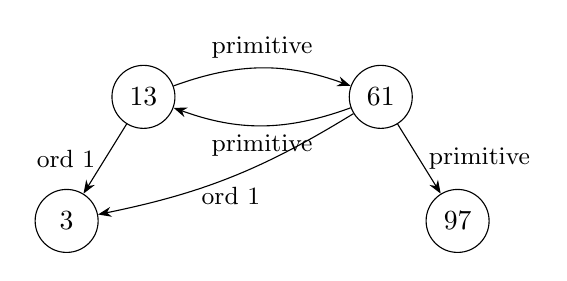
\begin{tikzpicture}[>=Stealth, node distance=2.2cm,
  v/.style={circle,draw,minimum size=8mm,inner sep=0pt}]
\node[v] (a) {$13$};
\node[v,right=of a] (b) {$61$};
\node[v,below left=1.0cm and 0.4cm of a] (c) {$3$};
\node[v,below right=1.0cm and 0.4cm of b] (d) {$97$};
\draw[->,bend left=20] (a) to node[above]{\small primitive} (b);
\draw[->,bend left=20] (b) to node[below]{\small primitive} (a);
\draw[->] (a) to node[left]{\small ord 1} (c);
\draw[->] (b) to[bend left=10] node[below]{\small ord 1} (c);
\draw[->] (b) to node[right]{\small primitive} (d);
\end{tikzpicture}
\end{center}
All edges have weight $1$. ($61\equiv 1\pmod 3$, so $61\to 3$ is an
order-one edge.)
\end{example}

\begin{example}[A layer that folds downward]
$\Phi_3(67)=67^2+67+1=4557=3\cdot 7^2\cdot 31$: every prime factor is
smaller than $67$.
\end{example}

\begin{lemma}[Obligation capacity]\label{lem:L4}
For each $r\in S$,
\[
\#\{q\in Q:\ \ord_r(q)>1,\ \ord_r(q)\mid e_q\}\le a_r,\tag{L4}
\]
and globally $\sum_{q\in Q}(\sigma_0(e_q)-1)\le\Omega(N)$.
\end{lemma}

\paragraph{Why this is a capacity statement.}
Every source $q$ counted on the left contributes at least one copy of $r$ to
$\sigma(q^{a_q})$, hence at least one unit to the incoming weight at $r$.
But Lemma~\ref{lem:L1} says that the \emph{entire} incoming budget at $r$ is
only $a_r$.  Therefore at most $a_r$ different sources can each demand even
one unit from $r$.  The inequality deliberately throws away multiplicity and
is consequently quite coarse.

For example,
\[
\sigma(3^4)=121=11^2,
\]
so the single obligation $(3,5)$ lands at $11$ with weight $2$.  In the Hall
count it consumes only one ``obligation slot,'' even though arithmetically it
uses two units of $11$-adic capacity.  This illustrates both the usefulness
and the weakness of the unweighted obligation count: it detects overcrowding
of targets, but it forgets how expensive some assignments actually are.

\begin{lemma}[Logarithmic cut identity]\label{lem:L5}
$\delta_q>0$ for $q\in Q$, $\delta_p<0$, $\sum_s\delta_s=0$, and for
every $T\subseteq S$,
\[
\sum_{s\in T}\delta_s=L(T,S\setminus T)-L(S\setminus T,T).\tag{L5}
\]
\end{lemma}

\begin{proof}
$\delta_q>0$ since $\sigma(q^a)>q^a$. For $p$:
$\sigma(p^\alpha)/p^\alpha<p/(p-1)\le 5/4<2$ since $p\ge5$.
$\sum\delta_s=\log\prod\Sigma_s-\log N=0$. For (L5), write
$\log\Sigma_s=\sum_r w(s,r)\log r$ and $a_r=\sum_s w(s,r)$ by (L1):
\[
\sum_{s\in T}\delta_s=L(T,S)-\sum_{r\in T}a_r\log r=L(T,S)-L(S,T),
\]
and the edges inside $T$ cancel.
\end{proof}

\begin{lemma}[Orientation toward the Euler prime]\label{lem:L6}
If $\varnothing\ne T\subseteq S\setminus\{p\}$, then
$L(T,S\setminus T)>L(S\setminus T,T)$. Consequently every $q\in S$ has a
directed path to $p$, and the condensation of $G_N$ has a unique sink
strong component, which contains $p$.
\end{lemma}

\begin{proof}
The inequality is (L5) with all $\delta_q>0$. If $T$ is the set of
vertices with no path to $p$, then $T$ has no out-edges, so
$L(T,S\setminus T)=0\le L(S\setminus T,T)$, forcing $T=\varnothing$.
\end{proof}

\paragraph{A singleton example.}
Take a nonspecial component $13^2$.  Its local divisor sum is
$\sigma(13^2)=183=3\cdot61$, so its outgoing logarithmic mass is
$\log 3+\log61=\log183$, whereas its exponent demand is
$2\log13=\log169$.  Their difference is
\[
\delta_{13}=\log\frac{183}{169}>0.
\]
Thus, if $13^2$ occurred in an OPN, the singleton cut $T=\{13\}$ would
export slightly more logarithmic mass than it imports.  Lemma~\ref{lem:L6}
says that the same phenomenon holds for \emph{every} set consisting only of
nonspecial vertices: after all internal exchanges cancel, that set must have
a net logarithmic export.  The Euler prime is therefore not merely a
convenient distinguished vertex; it is the only place where the accumulated
surplus can finally be absorbed.


\begin{remark}[A directed Matrix--Tree consequence]
Lemma~\ref{lem:L6} says that every vertex can reach the Euler prime $p$.
Consequently the support digraph of $G_N$ contains a directed spanning
in-arborescence rooted at $p$: for example, choose from each $q\ne p$ one
edge that decreases the directed distance to $p$.  The directed
Matrix--Tree theorem~\cite{Chaiken} therefore gives a positive weighted
cofactor for the \emph{out-degree} Laplacian
$L_{\rm out}=D_{\rm out}-W$ corresponding to such rooted arborescences.
This is a canonical graph invariant suggested by the distinguished Euler
sink.  It should not, however, be confused with the arithmetic operator
$D-W$ used later: there $D=\operatorname{diag}(a_s)$ is the in-degree/demand
matrix supplied by perfectness, not the out-degree matrix.  Any use of
Matrix--Tree cofactors in the OPN problem therefore needs an arithmetic
bridge between these two diagonals.
\end{remark}

\paragraph{Reaching $p$ versus being reached from $p$.}
Lemma~\ref{lem:L6} says that every vertex can \emph{reach} the Euler prime.
It is natural to ask about the reverse direction: can every vertex be reached
\emph{from} $p$?  If so, $G_N$ is strongly connected.  The logarithmic
identities alone do not settle this, because a set $A$ that receives no edges
from outside could still export a positive amount of logarithmic mass, which
is perfectly consistent with (L5).  The missing ingredient is integrality.
The following result is not part of the original post; it is added here
because it answers a question raised by the graph formulation itself.

\begin{proposition}[Strong connectivity]\label{prop:strong}
For every nonempty proper subset $A\subsetneq S$ there is an edge of $G_N$
from $S\setminus A$ into $A$.  Equivalently, $G_N$ is strongly connected.
\end{proposition}

\begin{proof}
Suppose no edge enters $A$.  Then every $t\in A$ receives its whole demand
$a_t$ from inside $A$, i.e.\ $a_t=\sum_{s\in A}w(s,t)$.  Let
$N_A=\prod_{t\in A}t^{a_t}$ be the corresponding unitary divisor.  Then
\[
\prod_{s\in A}\Sigma_s
=\prod_{t\in S}t^{\sum_{s\in A}w(s,t)}
=N_A\cdot M,
\qquad
M=\prod_{t\notin A}t^{\sum_{s\in A}w(s,t)}\in\mathbb Z .
\]
Since $\sigma(N_A)=\prod_{s\in A}\sigma(s^{a_s})$ equals
$2\prod_{s\in A}\Sigma_s$ if $p\in A$ and $\prod_{s\in A}\Sigma_s$ otherwise,
the abundancy $h(N_A)=\sigma(N_A)/N_A$ is an \emph{integer}, and it exceeds
$1$ because $A\ne\varnothing$.  On the other hand $h$ is multiplicative on
coprime arguments, so
\[
2=h(N)=h(N_A)\,h(N/N_A),
\]
and $h(N/N_A)>1$ because $A\ne S$.  Hence $1<h(N_A)<2$, which is impossible
for an integer.  Finally, a digraph is strongly connected exactly when every
nonempty proper vertex set has an entering edge (take $A$ to be the set of
vertices not reachable from a fixed vertex).
\end{proof}

\begin{remark}[Why the argument needs $k=2$]
The proof uses only that no integer lies strictly between $1$ and $2$.  For
the even perfect numbers the conclusion is visible directly: the graph on
$\{2,M_p\}$ is the directed $2$-cycle $2\rightleftarrows M_p$ (see
Example~\ref{ex:even}).  For a $k$-perfect number with $k\ge3$ the
same argument only shows that a closed set $A$ would give a unitary divisor
with integral abundancy $h(N_A)<k$, which is not a contradiction by itself.
\end{remark}

The Euler prime is the unique \emph{sink} of the logarithmic flow
(Lemma~\ref{lem:L6}), but Proposition~\ref{prop:strong} shows that it is not
a sink of the \emph{graph}: there are edges out of $p$ leading back to every
vertex.  Strong connectivity has a pleasant linear-algebra consequence.

\begin{corollary}[Rank of the Poisson operator]\label{cor:rank}
Let $L=D-W$ with $D=\operatorname{diag}(a_s)$.  Then the left nullspace of
$L$ is spanned by $\one$, and $\operatorname{rank}L=\omega(N)-1$.
Consequently $Lx=b$ is solvable exactly when $\one^{\mathsf T}b=0$, and its
solution is unique up to adding a vector in the one-dimensional kernel of $L$.
\end{corollary}

\begin{proof}
A row vector $y^{\mathsf T}$ satisfies $y^{\mathsf T}L=0$ iff
\[
y_r=\sum_{s\in S}\frac{w(s,r)}{a_r}\,y_s\qquad(r\in S),
\]
i.e.\ $y=My$ with $M=D^{-1}W^{\mathsf T}$.  By (L1) every row of $M$ sums to
$1$, so $M$ is the transition matrix of a Markov chain that walks
\emph{backward} along the edges of $G_N$, and $y$ is a harmonic function for
it.  By Proposition~\ref{prop:strong} this chain is irreducible.  At a vertex
where $y$ attains its maximum, $y_r$ is an average of the values at its
backward neighbors, so all of them are maximal too; by irreducibility the
maximum spreads to every vertex and $y$ is constant.  Hence the left
nullspace is $\mathbb R\one$ and the rank is $|S|-1$.
\end{proof}

For example, $\ell=(\log s)_{s\in S}$ is pinned down by the equation
$L\ell=-\delta$ of Section~\ref{sec:poisson} up to a single additive direction.  This settles a
point that would otherwise need a separate hypothesis: the Fredholm condition
$\sum_s\delta_s=0$ is not merely necessary but sufficient for solvability.
The additive direction itself, the kernel of $L$, turns out to carry
interesting integer structure: it is an \emph{arithmetical structure} in the
sense of Lorenzini.  Section~\ref{sec:arithmetical} develops this.

\begin{lemma}[Maximal prime]\label{lem:L7}
Let $R=\max S$. If $q\in Q$, $q<R$, supplies $R$, then
$R\nmid e_q/\ord_R(q)$, so $w(q,R)=v_R(q^{\ord_R(q)}-1)$. Also the
number of such suppliers is at most $h_R-1$, where
$h_R=(R-1)/2^{v_2(R-1)}$ is the order of the odd-order subgroup of
$(\Z/R\Z)^\times$.\hfill(L7), (7.1)
\end{lemma}

\paragraph{Why the largest prime is special.}
For a general target $r$, an edge can gain extra weight from the multiplier
term $v_r(e_q/\ord_r(q))$ in Lemma~\ref{lem:L2}.  At the largest prime $R$
this mechanism is severely constrained.  If $R$ divided that multiplier,
then $e_q\ge R\ord_R(q)>R$.  Zsigmondy applied at the larger exponent $e_q$
would force a primitive divisor $\ell\equiv1\pmod{2e_q}$, hence
$\ell>R$, contradicting maximality.  Thus incoming weight at $R$ has to come
from the base-order term rather than from arbitrarily repeated multiplier
lifting.

A small numerical model shows the idea.  Since
\[
\sigma(5^2)=31,
\]
we have $\ord_{31}(5)=3$, so an exponent with $e_5=3$ can supply the target
$R=31$.  But if one tried to obtain an extra factor of $31$ from a multiplier
by taking, say, $e_5=3\cdot31=93$, then a primitive divisor of $5^{93}-1$
would be at least $2\cdot93+1=187>31$.  Such a prime could not fit in a
prime set whose maximum is $31$.

The subgroup bound has a similar interpretation.  Any supplier of $R$ has
odd multiplicative order modulo $R$, so its residue lies in the odd-order
subgroup of $(\Z/R\Z)^\times$.  For the toy value $R=31$, this subgroup has
order $h_R=15$; excluding the identity residue leaves at most $14$ possible
nontrivial supplier residues.  For actual OPN bounds $R$ is enormous, so this
count is usually far too weak numerically, but it explains the group-theoretic
content of the lemma.

\begin{lemma}[Cheap-edge capacity]\label{lem:L8}
If all weights were $0$ or $1$, then
$\Omega(N)=\sum_{s,r}w(s,r)\le\omega(N)(\omega(N)-1)$.
\end{lemma}

\paragraph{Concrete meaning.}
A loopless digraph on $k$ vertices has at most $k(k-1)$ directed edges.  If
every edge carries only one unit of valuation, the total incoming valuation
available in the whole graph is therefore at most $k(k-1)$.  But by
Lemma~\ref{lem:L1} that total is exactly $\Omega(N)$.

For instance, Nielsen's theorem permits the extremal possibility
$\omega(N)=10$, but then a $0/1$-weighted $\sigma$-graph could carry at most
$10\cdot9=90$ units.  The published bound $\Omega(N)\ge101$ already exceeds
$90$.  Consequently, if an OPN with exactly ten distinct prime factors
existed, \emph{some edge would necessarily have weight at least $2$}.  In
arithmetic language, at least one local divisor sum would have to contain the
square of another prime divisor of $N$.  The limitation is that
$k(k-1)$ grows quadratically while known lower bounds for $\Omega$ grow only
linearly in $k$, so this neat contradiction does not persist for arbitrary
$k$: already for $k=11$ the capacity is $110\ge101$.\footnote{Rodgers'
preprint gets this comparison wrong in two opposite ways.  Its \S8.1 says
that $\Omega(N)\ge101$ is compatible with the cheap-only bound ``for the
known ranges of $\omega(N)$,'' which fails at $\omega(N)=10$, where the
capacity is $90<101$.  Its Appendix~C.4 says that $\omega(N)\ge10$ makes the
capacity equal to $90$ and so ``rules out the pure cheap-only scenario,''
which fails for every $\omega(N)\ge11$.  The correct statement is the one in
the text: an expensive edge is forced when $\omega(N)=10$, and nothing is
forced by this count alone when $\omega(N)\ge11$.}

The post compares this with published bounds: $\omega(N)\ge10$ (Nielsen
\cite{Nielsen}), $\Omega(N)\ge101$ (Ochem--Rao~\cite{OR2012}), and
$\Omega(N)\ge2\omega(N)+51$ (Ochem--Rao~\cite{OR2014}).  Ochem's current
computational project page reports that the searches have since been pushed
to $N>10^{2200}$ and $\Omega(N)\ge115$~\cite{OchemWeb}; these should be
distinguished from the older published $10^{1500}$ and $101$ theorems.
A linear lower bound on $\Omega$ can never beat the quadratic cheap-edge
capacity by itself, so counting edges alone will not suffice.

\subsection{The two ``breakthrough lemmas''}

The following two statements were proposed as possible endgames.  They are
called ``breakthrough'' lemmas because either one, if proved under the stated
hypotheses, would rule out OPNs.  That is also the reason for caution: the
hypotheses already encode so much of perfectness that the statements are
closer to reformulations of the original problem than to presently accessible
lemmas.  It is nevertheless useful to spell them out, because they identify
\emph{what kind of obstruction} a graph-theoretic proof would need.

\begin{claim}[A: Cyclotomic Hall deficiency]
For every Euler-form prime set satisfying $\sigma$-closure, (L1) and
(L2), there is a family $\mathcal A\subseteq\mathcal O$ with
\[
|\mathcal A|>\sum_{r\in U(\mathcal A)}a_r,
\qquad U(\mathcal A)=\bigcup_{(q,d)\in\mathcal A}P(q,d).\tag{H}
\]
\end{claim}

\paragraph{What Claim A is trying to say.}
Think of the cyclotomic obligations $(q,d)$ as jobs that must be assigned to
prime vertices.  Zsigmondy guarantees that every job has at least one
primitive-prime target.  A target $r$ has capacity $a_r$, because each job
assigned to $r$ contributes at least one unit to the incoming valuation at
$r$, and the total incoming valuation is exactly $a_r$ by (L1).  Thus the
primitive-prime incidence relation gives a bipartite matching problem with
capacitated right-hand vertices.

Hall's theorem says that such an assignment can exist only if every family of
jobs has enough total neighboring capacity.  In the present notation the
necessary inequality is
\[
|\mathcal A|\le \sum_{r\in U(\mathcal A)}a_r.
\]
Claim A asserts that the arithmetic always forces some family for which the
reverse strict inequality holds.  Such a family would be a certificate that
the cyclotomic obligations cannot all be absorbed by the available primes.

\begin{example}[A toy Hall obstruction]
Suppose five obligations $A_1,\dots,A_5$ can land only at two nonspecial
prime vertices $r_1,r_2$, each carrying the minimal exponent
$a_{r_1}=a_{r_2}=2$.  Then their neighborhood has total capacity $4$, while
there are $5$ obligations:
\[
5>2+2.
\]
No assignment is possible, regardless of how the five jobs are routed.
This is exactly the combinatorial shape Claim A seeks inside an OPN.  The
example is schematic---actual target sets are determined by multiplicative
orders---but its capacities are compatible with Euler form.
\end{example}

The arithmetic version is subtler because target sets usually overlap in
complicated ways and capacities need not be $1$.  For example,
\[
\Phi_5(3)=121=11^2.
\]
The obligation $(3,5)$ has primitive target $11$.  Hall's count records one
job assigned to a vertex of capacity $a_{11}$, while the actual factorization
uses two units of $11$-adic valuation.  Thus the unweighted Hall model is a
\emph{relaxation}: it intentionally forgets some expensive multiplicity.

\paragraph{Why the stated hypothesis is too ambitious.}
An actual OPN already satisfies $\sigma$-closure and exact valuation balance.
Therefore proving that \emph{every} such configuration violates Hall is, in
effect, proving that no OPN exists.  A more realistic intermediate target is
to impose only a selected family of obligations and derive a structural
inequality.  For example, one could use only the level-$3$ obligations from
vertices with $a_q=2$, where
\[
\Phi_3(q)=q^2+q+1,
\]
and try to prove that too many such low-exponent vertices cannot share a
small set of targets.  A theorem of the schematic form
\[
\#\{q:a_q=2\}\le C\,\#\{r:a_r\ge4\}+C_0
\]
would not prove nonexistence, but it would immediately yield a new lower
bound on $\Omega/\omega$.  This is the kind of weakened Hall statement that
could feed the discharging program in Section~\ref{sec:approach}.

\begin{claim}[B: Recycling capacity]
Every $\sigma$-closed, valuation-balanced Euler-form configuration
satisfies $E(N)\le 51$.
\end{claim}

\paragraph{What exponent excess measures.}
The smallest exponents compatible with Euler's form are
\[
\alpha=1,\qquad a_q=2\quad(q\in Q).
\]
If $k=\omega(N)$, this baseline has
\[
\Omega_{\min}=1+2(k-1)=2k-1,
\]
so $E(N)=\Omega(N)-(2\omega(N)-1)$ measures exactly how far the exponent
pattern lies above the minimal Euler pattern.  Raising one nonspecial
exponent from $2$ to $4$ adds $2$ to $E$; raising the Euler exponent from
$1$ to $5$ adds $4$.

For example, with ten distinct prime factors the minimal Euler pattern would
have $\Omega=19$ and $E=0$.  If one nonspecial component had exponent $4$
instead of $2$, then $\Omega=21$ and $E=2$.  At the opposite extreme, a
single nonspecial exponent $54$ in place of $2$ would contribute the full
$52$ units of excess by itself.  More generally, across a larger prime set,
twenty-six separate increases from exponent $2$ to exponent $4$ would also
contribute $52$.

Ochem--Rao's published inequality
\[
\Omega(N)\ge2\omega(N)+51
\]
is exactly the statement
\[
E(N)\ge52.
\]
Thus Claim B, which says $E(N)\le51$, would contradict a known theorem by one
unit and finish the OPN problem.

\paragraph{Where ``recycling'' enters.}
Increasing an exponent changes $e_q=a_q+1$ and usually creates additional
cyclotomic layers $\Phi_d(q)$.  Zsigmondy often forces primitive prime
factors for those layers.  The hoped-for charging argument is that a finite
prime set cannot keep reusing the same vertices to absorb all of these new
requirements without exhausting their valuation capacities.  The difficulty
is that divisor counts grow slowly, primitive primes can be recycled across
different bases, and high-weight edges can absorb more than one valuation
unit at a time.  No known argument turns this intuition into the universal
constant $51$.

\paragraph{A more realistic weaker target.}
Instead of bounding $E(N)$ by an absolute constant, try to control how much
excess can be supported by a specified number of high-exponent vertices.  For
example, let
\[
H=\#\{q\in Q:a_q\ge4\}.
\]
An inequality of the form
\[
\#\{q\in Q:a_q=2\}\le C H+C_0
\]
would already force a positive proportion of nonspecial vertices to have
exponent at least $4$, and hence improve a lower bound for
$\Omega/\omega$.  Restricted-exponent theorems provide evidence that such
questions can be tractable: Ochem--Zelinsky's restrained case, discussed in
Section~\ref{sec:assessment}, assumes that all but one nonspecial exponent are $2$ and obtains an
extraordinarily strong restriction on the exceptional component.

\paragraph{Logical status.}
Claim A and Claim B should therefore be read as \emph{targets that describe a
possible final obstruction}, not as established reductions of the OPN
conjecture.  The educational value of the graph model is that it suggests
weaker quantitative versions---capacity inequalities, forbidden local
configurations, and bounds on the proportion of low-exponent vertices---that
can be attacked without solving the whole problem at once.

%=====================================================================
\section{Assessment}\label{sec:assessment}
%=====================================================================

\subsection{What is correct}

Every numerical example and every proof sketch in Section~\ref{sec:program} checks out.
Example~\ref{ex:13} is a genuine counterexample to Theorem~5.1 of
Rodgers~\cite{Rodgers} as stated there.  The other results that the program
takes from the preprint---valuation balance, the LTE decomposition for edges
of order greater than $1$, primitive edges, the layer count
$\sigma_0(e_q)\le\omega(N)$, and the maximal-prime statement---are correct.
Lemma~\ref{lem:L2}, which adds the missing order-one case, is the right
foundation for any work with $\sigma$-graphs.

\subsection{Where the novelty is overstated}

\begin{itemize}[leftmargin=1.5em]
\item \textbf{Lemma~\ref{lem:L5} is multiplicativity of abundancy.} For
  $T\subseteq S$ let $N_T=\prod_{s\in T}s^{a_s}$ be the corresponding
  unitary divisor. Then $\sum_{s\in T}\delta_s=\log h(N_T)$, with the
  factor $2$ removed from $p$'s term if $p\in T$. The cut identity
  rewrites ``$h(N_T)>1$ and $\sigma(N_T)$ factors over $S$'' as flow.

\item \textbf{Lemma~\ref{lem:L6} is classical in substance.} It is
  equivalent to: if $M$ is a unitary divisor of $N$ with $p\nmid M$, then
  $\sigma(M)$ has a prime factor not dividing $M$. The SCC phrasing is
  pleasant but not new arithmetic.  The same is true of our own
  Proposition~\ref{prop:strong}: it is the graph form of the classical fact
  that a proper unitary divisor $M$ of a perfect number cannot satisfy
  $M\mid\sigma(M)$, because $1<h(M)<2$.  What the graph language adds is the
  \emph{consequence}---irreducibility, and hence the rank statement of
  Corollary~\ref{cor:rank}---rather than new arithmetic.

\item \textbf{Lemma~\ref{lem:L7} is weaker than a classical bound.} A
  primitive prime for $q^{e_q}-1$ is $\ge 2e_q+1$ and lies in $S$, so
  \[
  2e_q+1\le R\qquad\text{for every }q\in Q.
  \]
  In particular $R\nmid e_q$, which already gives $R\nmid e_q/\ord_R(q)$.
  This applies equally to Rodgers' Theorem~7.2, the source of the lemma,
  which uses only the weaker bound $\ell\ge e_q+1$ for a primitive prime
  $\ell$ even though, $\ell$ and $e_q$ both being odd, $\ell\equiv1\pmod{2e_q}$
  (as the preprint itself notes in its Appendix~A.2).

\item \textbf{The count (7.1) is useless in practice.} The largest prime
  factor of an OPN exceeds $10^8$ (Goto--Ohno \cite{GotoOhno}), so
  $h_R-1$ is vastly larger than any plausible $\omega(N)$.

\item \textbf{The global inequality in Lemma~\ref{lem:L4} is a
  tautology.} Since $\sigma_0(e)\le e$, we have $\sigma_0(e_q)-1\le e_q-1=a_q$,
  hence $\sum_q(\sigma_0(e_q)-1)\le\sum_q a_q\le\Omega(N)$ for \emph{any}
  exponents whatsoever. This is a warning sign for the Hall framing.
\end{itemize}

\subsection{The main problem: equivalence, not reduction}

\paragraph{Claim A.} The hypotheses ``$\sigma$-closure + (L1) +
Euler form'' are just $\sigma(N)=2N$ written prime by prime. So the
configurations Claim~A quantifies over \emph{are} odd perfect numbers,
and Claim~A says ``every OPN violates a necessary condition,'' i.e.\
``no OPN exists.'' A reformulation helps only if one proves deficiency
from a \emph{strict subset} of the constraints. But the unit-demand
relaxation (H) is almost certainly satisfiable:
\begin{itemize}[leftmargin=1.5em]
\item capacities $a_r$ grow linearly in the exponents;
\item demands $\sigma_0(e_q)-1$ grow like a divisor function;
\item the tautology above shows the global inequality has built-in slack.
\end{itemize}
The binding information is \emph{size}: $\Phi_d(q)\approx q^{\varphi(d)}$
must be absorbed \emph{completely} by $S$ with bounded exponents. Restoring
it gives a weighted flow with demand $\log\Phi_d(q)$ and capacity
$a_r\log r$, which is (L5) plus the full factorization, i.e.\ the
original problem.

\paragraph{Claim B.} ``OPNs have small exponent excess'' contradicts
known lower bounds, so it is as hard as nonexistence. The real precedent
is the special-exponent literature: Steuerwald \cite{Steuerwald} ruled
out all $\beta_q=1$, Kanold \cite{Kanold} ruled out all $\beta_q=2$, and
later work by McDaniel, Hagis, Cohen--Williams and others treated further
restricted patterns. Even those cases took real effort. The proposed
charging scheme needs a recycling bound independent of $\omega(N)$, and
nothing in the program supplies one.


A striking recent illustration of how rigid a restricted exponent pattern can
be is due to Ochem--Zelinsky~\cite{OchemZelinsky2026}.  They call an OPN
\emph{restrained} when all nonspecial even exponents are $2$ except one.  In
that situation the exceptional component must be a power of $3$, and its
exponent is at least $23{,}000{,}000{,}000$.  This does not approach the full
nonexistence problem, but it is strong evidence that the ``local type +
reducible configuration'' philosophy in Section~\ref{sec:approach} can extract serious
arithmetic information from nearly minimal exponent patterns.


\subsection{Why the obvious spectral normalization is weak}

The original Gemini/Argon proposal suggested normalized Laplacians and
Cheeger-type expansion.  There is a simple reason that the most immediate
normalization does not itself create a contradiction.  From (L1), the sum of
column $r$ of $W$ is $a_r$.  Hence
\[
P=WD^{-1}
\]
is column-stochastic:
\[
\one^{\mathsf T}P=\one^{\mathsf T}.
\]
Since $P$ is nonnegative, its spectral radius is therefore
$\rho(P)=1$, and $I-P$ automatically has eigenvalue $0$.  By
Proposition~\ref{prop:strong}, $P$ is moreover irreducible, so by
Perron--Frobenius this eigenvalue is simple.  Thus the basic Perron
eigenvalue is forced by valuation balance and strong connectivity, and
contains no new arithmetic information.

\paragraph{A two-vertex caricature.}
The point is easiest to see in a purely graph-theoretic toy example.  The
column-stochastic matrix
\[
P=\begin{pmatrix}0&1\\[2pt]1&0\end{pmatrix}
\]
has eigenvalues $1$ and $-1$, while
\[
P=\begin{pmatrix}1/2&1/2\\[2pt]1/2&1/2\end{pmatrix}
\]
has eigenvalues $1$ and $0$.  Stochasticity forces the eigenvalue $1$ but
places very different constraints on the rest of the spectrum.  Therefore a
spectral proof would need an arithmetic theorem explaining why matrices that
come from cyclotomic valuations cannot have the ``wrong'' second eigenvalue;
the normalization alone cannot provide that theorem.

One could still study a second eigenvalue, a singular-value gap, or one of the
directed normalized Laplacians of Chung~\cite{Chung2005}.  But any useful
bound would have to come from the number-theoretic restrictions on the
\emph{entries} of $W$---multiplicative orders, cyclotomic layers, and LTE---not
from stochasticity alone.  In particular, there is no evident uniform
Cheeger gap: the logarithmic divergences satisfy
\[
0<\delta_q<\log\frac{q}{q-1}\sim\frac1q,
\]
so large-prime vertices naturally permit cuts that are very nearly balanced
in the logarithmic flow.  This is why the later discharging and local
configuration program seems more concrete than beginning with a normalized
Laplacian.

\subsection{Sanity filters}

\paragraph{Spoofs.}
Spoof odd perfect numbers exist (Section~\ref{sec:perfect}).  Any argument
that does not use the primality of each base may therefore also ``prove''
that spoofs are impossible, which would be a contradiction.  Recall the
Descartes spoof $D=3^2\cdot7^2\cdot11^2\cdot13^2\cdot22021$ of
Example~\ref{ex:descartes}.

The log identities (L5)--(L6) hold for the spoof if $22021$ is treated
as a single vertex: they only use $\prod\Sigma_s=D$. Valuation balance
(L1) and the order arguments of Lemmas~\ref{lem:L2}--\ref{lem:L4} and
\ref{lem:L7} do distinguish real primes. So these are where primality
does real work.

\begin{example}[A logarithmic $5\times5$ aggregation of the Descartes spoof]\label{ex:descartes_lap}
The Descartes spoof
$D=3^2\cdot7^2\cdot11^2\cdot13^2\cdot22021$ from
Example~\ref{ex:descartes} satisfies
$22021=19^2\cdot61$.  Treating $C=22021$ as a single pseudo-prime cannot
produce an honest valuation matrix, because $v_C$ is not a prime-adic
valuation.  It does, however, produce an exact \emph{logarithmic}
aggregation.

Put
\[
\theta=\frac{\log19}{\log C},\qquad
\psi=\frac{\log61}{\log C}.
\]
Since $C=19^2\cdot61$,
\[
2\theta+\psi=1.
\]
The identities
\[
\begin{aligned}
\Sigma_3&=13, &
\Sigma_7&=3\cdot19=3C^{\theta},\\
\Sigma_{11}&=7\cdot19=7C^{\theta}, &
\Sigma_{13}&=3\cdot61=3C^{\psi},\\
\Sigma_C&=(C+1)/2=7\cdot11^2\cdot13
\end{aligned}
\]
therefore yield, in the coordinate order $(3,7,11,13,C)$, the real matrix
\[
L_{\rm eff}=\begin{pmatrix}
 2 &  0 &  0 & -1 &  0 \\
-1 &  2 &  0 &  0 & -\theta \\
 0 & -1 &  2 &  0 & -\theta \\
-1 &  0 &  0 &  2 & -\psi \\
 0 & -1 & -2 & -1 &  1
\end{pmatrix}.
\]
Its columns sum to zero precisely because $2\theta+\psi=1$, and with
$\ell=(\log3,\log7,\log11,\log13,\log C)^{\mathsf T}$ it satisfies the
same formal Poisson equation $L_{\rm eff}\ell=-\delta$ for the five spoof
components.

The point is diagnostic: $L_{\rm eff}$ has \emph{real logarithmic
coefficients}, not prime-adic valuation weights.  The earlier values
$1/2,1/2$ would not reproduce $\log19$ and $\log61$ and hence do not give
the correct Poisson equation.  Splitting $C$ into its true prime factors
$19$ and $61$ also does not create a genuine six-prime $\sigma$-graph for
the spoof, because the outgoing pseudo-prime local sum $(C+1)/2$ is not
$\sigma(19^2)\sigma(61)$.  This is exactly the arithmetic information lost
when a composite is allowed to masquerade as a prime.
\end{example}

\paragraph{Relaxation feasibility.}
Before trying to prove that a class of configurations is infeasible, check by
computer that the \emph{relaxed} constraints really are infeasible.  A useful
workflow is to choose a small candidate prime set $S$, prescribe or bound the
exponents $a_s$, introduce integer variables $w(s,r)$, impose the exact
column balances (L1), and forbid edges that violate the order conditions of
Lemma~\ref{lem:L2}.  One may then solve the resulting integer or linear
feasibility problem without requiring every row to be the complete prime
factorization of an actual $\sigma(s^{a_s})$.

If this relaxed system already has no solution, the solver can often expose a
small dual or combinatorial certificate worth proving by hand.  If it
\emph{does} have solutions, that is equally informative: any proposed proof
using only those relaxed constraints cannot work, because the fake solution
exhibits exactly what arithmetic information has been discarded.  In this
sense computation is a sanity filter for the proof strategy, not evidence
for or against the existence of an actual OPN.

%=====================================================================
\section{A stronger graph-theoretic approach}\label{sec:approach}
%=====================================================================

No known graph-theoretic method currently approaches a proof of
nonexistence.  The realistic target is instead \emph{structural inequalities}:
bounds on how many primes can have small exponent, ratio bounds on
$\Omega/\omega$, restrictions on short $\sigma$-cycles, and the like.
Graph language already has a track record here: the weighted digraph of
Bibby--Vyncke--Zelinsky~\cite{BibbyVynckeZelinsky} is used to organize
$\sigma_{m,n}$-pair restrictions, while modern factor-chain/discharging
arguments prove quantitative bounds on prime factors.

\subsection{Discharging}

Ochem--Rao's inequalities $\Omega\ge(18\omega-31)/7$ and
$\Omega\ge2\omega+51$ \cite{OR2014} are discharging arguments in
disguise. (Ochem is a graph theorist.) One can make this explicit.

Zelinsky subsequently improved the asymptotic slope: if $3\mid N$ then
\[
\Omega(N)\ge \frac{66}{25}\omega(N)-5,
\]
while if $3\nmid N$ then
\[
\Omega(N)\ge \frac{302}{113}\omega(N)-\frac{286}{113}
\]
\cite{Zelinsky2021}.  Clayton and Hansen~\cite{ClaytonHansen} then improved
the slope again: for every OPN
\[
\Omega(N)\ge\frac{99}{37}\,\omega(N)-\frac{187}{37}
\qquad(99/37\approx2.676),
\]
and if $3\nmid N$,
\[
\Omega(N)\ge\frac{51}{19}\,\omega(N)-\frac{46}{19}
\qquad(51/19\approx2.684).
\]
Ochem's project page currently summarizes the state of the art as
$\Omega(N)\ge\max\bigl(115,\ 2\omega(N)+51,\ (99\omega(N)-187)/37\bigr)$,
the $115$ being an unpublished computational bound~\cite{OchemWeb}.  These
inequalities are useful benchmarks for any LP/discharging model derived
directly from $G_N$.

\begin{itemize}[leftmargin=1.5em]
\item \textbf{Charges.} Give $s\in S$ initial charge $c(s)=a_s-2$, so a
  low-exponent vertex ($a_q=2$) starts at $0$. A ratio bound
  $\Omega\ge\lambda\omega$ with $\lambda>2$ says low-exponent vertices
  cannot dominate.
\item \textbf{Rules.} Move charge along edges between low- and
  high-exponent vertices, and show every vertex ends with charge
  $\ge\varepsilon$.
\item \textbf{Rigid local structure.} If $a_q=2$ then
  $\Sigma_q=\Phi_3(q)=q^2+q+1$. If $q\equiv1\pmod3$ then
  $q^2+q+1\equiv3\pmod9$, so $v_3=1$; every other prime factor $r$ has
  $\ord_r(q)=3$, hence $r\equiv1\pmod 6$. The whole of $q^2+q+1$ must be
  absorbed by $S$.
\item \textbf{Reducible configurations become Diophantine equations.}
  Patterns such as $\Phi_3(q)=3r$, $\Phi_3(q)=r^k$, or a short cycle of
  $a=2$ vertices exchanging all their valuation reduce to
  Nagell--Ljunggren-type equations $\frac{x^n-1}{x-1}=y^m$ or to
  $S$-unit problems.  Three classical positive solutions of the former are
  \[
  \tfrac{3^5-1}{2}=11^2,\qquad \tfrac{7^4-1}{6}=20^2,\qquad
  18^2+18+1=7^3.
  \]
  The general Nagell--Ljunggren equation is \emph{not} completely solved;
  Bennett--Levin~\cite{BennettLevin} emphasize that proving completeness of
  the known list is beyond current methods, while obtaining strong
  restrictions on any further solution.  Thus a discharging proof may use
  classified small subcases, but should not silently assume a complete
  solution of the general equation.
\end{itemize}

\paragraph{What discharging is doing here.}
A discharging argument is bookkeeping: total charge is conserved while it is
moved between vertices according to local rules.  With the simple initial
choice $c(s)=a_s-2$, a nonspecial exponent-$2$ vertex has charge $0$, an
exponent-$4$ vertex has charge $2$, and an Euler vertex with $\alpha=1$ has
charge $-1$.  The total initial charge is
\[
\sum_s c(s)=\Omega(N)-2\omega(N).
\]
If arithmetic restrictions force high-exponent vertices to subsidize nearby
low-exponent configurations in such a way that every vertex finishes with a
positive average charge, then one obtains a lower bound on
$\Omega/\omega$.

A toy model makes the mechanism visible.  Ignore the special vertex and
suppose every vertex has exponent either $2$ or at least $4$, and suppose one
could prove the local structural inequality
\[
x_2\le2x_{\ge4},
\]
where $x_2$ and $x_{\ge4}$ count the two types.  Then, using the smallest
possible exponent in each class,
\[
\frac{\Omega}{\omega}
\ge \frac{2x_2+4x_{\ge4}}{x_2+x_{\ge4}}
\ge \frac83.
\]
The inequality $x_2\le2x_{\ge4}$ is hypothetical here; the point is that a
local graph restriction immediately turns into a global prime-factor bound.
A dual LP or a discharging proof is a systematic way to discover and certify
such inequalities.

This is the architecture of the Four Color Theorem proofs: an unavoidable
set of local configurations, each shown reducible, with discharging
connecting them.  In the OPN setting the ``reducibility'' step is
number-theoretic rather than planar-topological: one rules out a local
$\sigma$-graph pattern by congruences, multiplicative orders, cyclotomic
factorization, or a Diophantine equation.

\subsection{LP duality finds the rules}

\begin{enumerate}[leftmargin=1.5em]
\item Classify vertices into \emph{types}: exponent class
  ($a=2,4,6,\dots$, or special), small-prime residue data
  ($q\bmod3$, $q\bmod5$, \dots), and whether $q=R$.
\item Write (L1) and (L5) as linear constraints in the variables
  $x_t$ (number of vertices of type $t$) and $y_{t,t'}$ (total weight
  from type $t$ to type $t'$). Lemma~\ref{lem:L2} decides which
  $y_{t,t'}$ may be positive and with what minimum.
\item Minimize $\Omega/\omega=\sum_t a_t x_t/\sum_t x_t$ over the LP
  relaxation. The optimal dual solution \emph{is} a set of discharging
  rules.
\item The extremal primal solution shows which configurations are
  ``too cheap''; kill them with Diophantine or Zsigmondy arguments,
  add the exclusions as constraints, and re-solve.
\end{enumerate}
Each round is a certified improvement, checkable independently.

\paragraph{Why the dual solution is useful.}
The primal LP asks, in effect, ``what is the cheapest hypothetical mixture of
vertex types that obeys all currently known local rules?''  If the optimum is
too low, its extremal solution identifies the configuration responsible for
the weakness.  The dual LP assigns numerical prices to the constraints.  A
dual certificate can often be rewritten as a human discharging proof: the
``prices'' say how much charge each local rule is allowed to transfer.

For example, in the toy inequality $x_2\le2x_{\ge4}$ above, one may think of
a high-exponent vertex as having enough surplus to support at most two
low-exponent vertices.  The resulting $8/3$ bound is what a tiny two-type LP
would discover automatically.  A realistic OPN LP would have many more types
(residue classes, exponent classes, maximal-prime status, and perhaps
cyclotomic-layer data), but the logic is the same: solve the relaxation,
inspect the cheapest pattern, prove that pattern arithmetically impossible,
and add the corresponding inequality.

\subsection{Flow decomposition}

Weight edge $s\to r$ by $w(s,r)\log r$.  Each $q\ne p$ has in-flow
$a_q\log q$ and out-flow $a_q\log q+\delta_q$, with
$0<\delta_q<\log\frac q{q-1}$.  Thus the flow is a near-circulation
\emph{in divergence}: there are small sources at every $q\ne p$ and one
sink at $p$.  The standard flow-decomposition theorem writes a nonnegative
flow as directed cycles plus source-to-sink paths, and the total amount
\emph{injected} into the path part is $\sum_{q\ne p}\delta_q=-\delta_p$.
Small injected flow does not immediately mean small path \emph{mass}, because
a little flow could in principle travel along many edges.  But the paths in a
flow decomposition can be taken to be simple, and a simple path in a graph
with $\omega(N)$ vertices has at most $\omega(N)-1$ edges.  That is enough to
make the slogan ``most of the mass circulates'' precise.

\begin{proposition}[Most logarithmic mass lies on cycles]\label{prop:pathmass}
Decompose the flow $f(s,r)=w(s,r)\log r$ into simple directed cycles and
simple paths from the sources $q\ne p$ to the sink $p$.  The total edge mass
$\sum_{s,r}f(s,r)$ equals $\log N$, while the edge mass carried by the paths
is at most
\[
(\omega(N)-1)\log\frac{2p^\alpha}{\sigma(p^\alpha)}<(\omega(N)-1)\log2 .
\]
Consequently the fraction of the edge mass carried by cycles exceeds
\[
1-\frac{(\omega-1)\log2}{\log5+2(\omega-1)\log3}
\;>\;1-\frac{\log2}{2\log3}\;>\;0.68,
\]
and this fraction tends to $1$ as $\omega(N)\to\infty$.
\end{proposition}

\begin{proof}
By (L1), $\sum_{s,r}w(s,r)\log r=\sum_r a_r\log r=\log N$.  The path flows
add up to the total supply
$\sum_{q\ne p}\delta_q=-\delta_p=\log\bigl(2p^\alpha/\sigma(p^\alpha)\bigr)$,
which is less than $\log2$, and each path uses at most $\omega-1$ edges.  For
the denominator, $\log N=\sum_s a_s\log s\ge\log5+2\sum_{q\in Q}\log q$, and
the $\omega-1$ primes $q\in Q$ are distinct odd primes, so
$\sum_{q\in Q}\log q\ge(\omega-1)\log3$; in fact this sum grows like
$\omega\log\omega$, which gives the limit.
\end{proof}

For instance, with $\omega(N)=10$ the paths carry less than
$9\log2/(\log5+18\log3)\approx29\%$ of the logarithmic mass, so more than
$70\%$ of it travels around directed cycles.  This is a structural statement
only, but it justifies paying special attention to cycles:
\begin{itemize}[leftmargin=1.5em]
\item \emph{Short cycles are rigid.} The 2-cycle of
  Example~\ref{ex:cycle} exists, but a cycle carrying most of the
  valuation at both ends forces near-equalities
  $q^2+q+1=3^{\varepsilon}r^k\cdot(\text{small})$, which fall under
  $S$-unit bounds.
\item \emph{Long cycles force growth.} Primitive edges satisfy
  $\ell\equiv1\pmod{2d}$, and the maximal prime caps $2e_q+1\le R$.
\end{itemize}

\subsection{A concrete first project}

A useful first project should have an external benchmark: one should know in
advance what inequality the graph machinery ought to reproduce before asking
it to improve anything.  The following sequence provides such a test.

\begin{enumerate}[leftmargin=1.5em]
\item \textbf{Re-derive a known bound in graph language.}  Recast
  $\Omega\ge(18\omega-31)/7$ as an explicit discharging proof on $G_N$.
  The goal is not novelty; it is to verify that the chosen vertex types and
  local edge rules are rich enough to recover established arithmetic.
\item \textbf{Let an LP rediscover the same rules.}  Build the type-LP in
  Sage and compare its optimum with $18/7$.  If the LP gives a weaker slope,
  inspect its extremal solution to see exactly which arithmetic condition is
  missing.  If its dual reproduces the known discharging coefficients, that
  is evidence that the modeling choices are faithful.
\item \textbf{Add one genuinely arithmetic exclusion.}  Encode classified
  Nagell--Ljunggren or $S$-unit exclusions for selected $a=2$
  configurations and re-solve.  Any improvement in the optimum is then
  traceable to a specific theorem rather than to an opaque numerical search.
\end{enumerate}
Zelinsky's 2018 paper~\cite{Zelinsky} and the sharper 2021 result
\cite{Zelinsky2021} improve Ochem--Rao's $18/7$ slope by analyzing local
component/factor structures, and Clayton--Hansen~\cite{ClaytonHansen}
improve them further.  Any implementation should benchmark against the
current record slopes $99/37$ (general) and $51/19$ (when $3\nmid N$), as
well as the computational bounds reported by Ochem~\cite{OchemWeb}.

\subsection{Arithmetical structures on the $\sigma$-graph}\label{sec:arithmetical}

Corollary~\ref{cor:rank} says that the Poisson operator $L=D-W$ of an OPN
has a one-dimensional kernel and that its left kernel is spanned by $\one$.
This subsection identifies the kernel.  The right language is Lorenzini's
theory of arithmetical structures~\cite{Lorenzini}, recalled in
Section~\ref{sec:arithdefs}.  The upshot is that an
OPN $\sigma$-graph carries two arithmetical structures whose $S$-values are
both the exponent vector $a$: a trivial one on incoming edges, and a
canonical, nontrivial one on outgoing edges.

\subsubsection{The two structures on an OPN $\sigma$-graph}

\begin{proposition}[The in-structure is natural]\label{prop:instructure}
For an OPN, $(R,S)=(\one,a)$ is an in-structure on $G_N$, with generalized
Laplacian $L=D-W$.
\end{proposition}

\begin{proof}
With $R\equiv1$ the defining identity reads $a_r=\sum_s w(s,r)$, which is
valuation balance (Lemma~\ref{lem:L1}).
\end{proof}

Since $a_r$ is the weighted in-degree of $r$, this is the directed analogue
of the natural structure $R\equiv1$, $S=\deg$.  It contains no new
information; it is (L1) in different clothing.  The out-direction is more
interesting.

\begin{theorem}[The canonical out-structure]\label{thm:outstructure}
Let $N$ be an OPN.  There is a unique positive integer vector
$R_N=(R_N(s))_{s\in S}$ with $\gcd R_N=1$ such that $(R_N,a)$ is an
out-structure on $G_N$:
\[
a_s\,R_N(s)=\sum_{r\in S}w(s,r)\,R_N(r)\qquad(s\in S).
\]
Equivalently, $R_N$ spans $\ker L$.
\end{theorem}

\begin{proof}
The matrix $D^{-1}W=D^{-1}(WD^{-1})D$ is similar to $WD^{-1}$, which is
column-stochastic by (L1), so its spectral radius is $1$.  By
Proposition~\ref{prop:strong} the digraph $G_N$ is strongly connected, so
$D^{-1}W$ is irreducible.  The Perron--Frobenius theorem (compare the
undirected version in the subsection ``Perron--Frobenius'' of the chapter
``Applications to graph spectra'' of~\cite{MJappl}) gives a positive vector
$x$ with $D^{-1}Wx=x$, i.e.\ $Lx=0$, unique up to scaling.  Because $L$ has
integer entries and rank $\omega(N)-1$ (Corollary~\ref{cor:rank}), its
kernel is spanned by a rational vector; scaling $x$ to a primitive integer
vector gives $R_N$.
\end{proof}

So the single integer matrix $L=\operatorname{diag}(a)-W$ is simultaneously
the generalized Laplacian of a trivial in-structure (left kernel $\one$) and
of a nontrivial out-structure (right kernel $R_N$).  In the symmetric theory
of~\cite{MJappl} these two kernels coincide; here they need not.

\begin{corollary}[Properties of $R_N$]\label{cor:RN}
Let $N$ be an OPN.
\begin{enumerate}[label=(\alph*)]
\item $R_N\equiv\one$ if and only if $\Omega(\Sigma_s)=a_s$ for every
  $s\in S$, i.e.\ if and only if every vertex of $G_N$ has equal weighted
  in- and out-degree.
\item The solutions of $Lx=-\delta$ are exactly the vectors
  $\ell+tR_N$, $t\in\mathbb R$, where $\ell=(\log s)_{s\in S}$.
\item $\operatorname{coker}L\cong\mathbb Z\oplus K(N)$ for a finite abelian
  group $K(N)$, the arithmetical critical group of the out-structure.
\end{enumerate}
\end{corollary}

\begin{proof}
(a) $L\one=(a_s-\Omega(\Sigma_s))_s$, so $\one\in\ker L$ exactly when every
$a_s=\Omega(\Sigma_s)$; by uniqueness, this happens exactly when
$R_N=\one$.  (b) Corollary~\ref{cor:rank}.  (c) $L$ is an integer matrix of
rank $\omega(N)-1$; its Smith normal form has exactly one zero on the
diagonal.
\end{proof}

Part (a) gives a pleasant interpretation: $R_N$ measures how far the
$\sigma$-graph is from being \emph{Eulerian} (balanced), which is the same
defect $V_s=a_s-\Omega(\Sigma_s)$ that appears as the ``potential'' in the
quadratic-form identity of Section~\ref{sec:undirected}.  Part (b) says that
$R_N$ is exactly the ambiguity in the Poisson equation.  Part (c) attaches to
every hypothetical OPN a finite abelian group $K(N)$, about which nothing is
currently known.

\subsubsection{Examples from multiperfect numbers}

The same construction works for $k$-perfect numbers, using the vertex set
$\widehat S$ of Section~\ref{sec:multiperfect} and $S$-values
$a_s+v_s(k)$ (the column sums of $W$).  In the examples below every prime
of $k$ divides $N$, the digraph is strongly connected, and the kernel of
$\operatorname{diag}(a+v(k))-W$ is one-dimensional and spanned by a positive
vector; all of this was checked by computer.

\begin{example}[Even perfect numbers]\label{ex:arith-even}
For $N=2^{p-1}M_p$ the $\sigma$-graph is the $2$-cycle with $w(2,M_p)=1$
and $w(M_p,2)=p$, and the $S$-values are $(p,1)$.  The out-structure is
\[
R=(1,p),\qquad S=(p,1),
\]
since $p\cdot1=w(2,M_p)\cdot p$ and $1\cdot p=w(M_p,2)\cdot1$.  The
generalized Laplacian $\begin{pmatrix}p&-1\\-p&1\end{pmatrix}$ has Smith
normal form $\operatorname{diag}(1,0)$, so the critical group is trivial.
By Corollary~\ref{cor:RN}(a), $R\ne\one$ reflects the imbalance between
the in-degree $p$ and out-degree $1$ at the vertex $2$.
\end{example}

\begin{example}[$N=120$ and the triangle]\label{ex:arith-120}
For $120=2^3\cdot3\cdot5$ (Example~\ref{ex:120}), in the order $(2,3,5)$,
\[
W=\begin{pmatrix}0&1&1\\2&0&0\\1&1&0\end{pmatrix},\qquad
S=a+v(3)=(3,2,1).
\]
Solving $(\operatorname{diag}(S)-W)R=0$ gives $R=(1,1,2)$:
\[
3\cdot1=1\cdot1+1\cdot2,\qquad
2\cdot1=2\cdot1,\qquad
1\cdot2=1\cdot1+1\cdot1 .
\]
The underlying graph of this $\sigma$-graph is the triangle $C_3$, and $R$
is the same vector $(1,1,2)$ as in the arithmetical structure on $C_3$
in~\cite{MJappl}.  Only the $S$-values differ, $(3,2,1)$ instead of
$(3,3,1)$, because the edges now have directions and unequal weights.  The
Smith normal form of the generalized Laplacian is $\operatorname{diag}(1,2,0)$,
so $K(120)\cong\mathbb Z/2$.
\end{example}

\begin{center}
\begin{tabular}{@{}lclll@{}}
\toprule
$N$ & $k$ & primes & $R$ & $S$\\
\midrule
$2^{p-1}M_p$ & $2$ & $2,M_p$ & $(1,p)$ & $(p,1)$\\
$120$ & $3$ & $2,3,5$ & $(1,1,2)$ & $(3,2,1)$\\
$672$ & $3$ & $2,3,7$ & $(1,1,3)$ & $(5,2,1)$\\
$30240$ & $4$ & $2,3,5,7$ & $(1,2,3,3)$ & $(7,3,1,1)$\\
$32760$ & $4$ & $2,3,5,7,13$ & $(1,2,3,3,4)$ & $(5,2,1,1,1)$\\
$2178540$ & $4$ & $2,3,5,7,13,19$ & $(2,5,7,8,10,11)$ & $(4,2,1,2,1,1)$\\
\bottomrule
\end{tabular}
\end{center}

\noindent
The critical groups are $\mathbb Z/2$ for $120$, $672$, $30240$ and
$32760$, and trivial for the even perfect numbers and for $2178540$.

\subsubsection{Equitable quotients force $R_N$ to be constant on cells}

The pullback construction of~\cite{MJappl} transports an arithmetical
structure from the target of a harmonic morphism to its source, with $R$
constant on fibers.  Because $R_N$ is \emph{unique}, this can be run
backwards to give a concrete obstruction to equitable quotients of $G_N$.

Call a partition $\pi$ of $S$ \emph{out-equitable} if for any two cells
$C,C'$ the row sum $\sum_{r\in C'}w(s,r)$ takes the same value $b_{CC'}$ for
every $s\in C$.  This is the directed form of the weighted equitable
partitions of the chapter ``Edge-weighted graph partitions''
of~\cite{MJappl}: each vertex of a cell sends the same total weight to each
cell.  (It is the transpose of the in-equitable condition of
Section~\ref{sec:hm}.)

\begin{proposition}[Descent of the canonical structure]\label{prop:descent}
Let $N$ be an OPN and let $\pi$ be an out-equitable partition of $S$ such
that the exponents $a_s$ are constant, say $a_C$, on each cell $C$.  Then
$R_N$ is constant on each cell, and $(R_N|_C,\,a_C)$ is an out-structure on
the quotient digraph with weight matrix $B=(b_{CC'})$, where the diagonal
entries $b_{CC}$ are recorded as loops.
\end{proposition}

\begin{proof}
Let $U$ be the space of vectors constant on cells.  Out-equitability says
$WU\subseteq U$, and $DU\subseteq U$ because $a$ is constant on cells, so
$LU\subseteq U$.  Since $\one^{\mathsf T}L=0$, the image $LU$ lies in the
proper subspace $U\cap\{x:\one^{\mathsf T}x=0\}$ of $U$, so $L|_U$ is not
surjective and hence has a nonzero kernel.  That kernel lies in
$\ker L=\mathbb RR_N$, so $R_N\in U$.  For $s\in C$,
$a_C R_N(C)=\sum_{C'}\sum_{r\in C'}w(s,r)R_N(C')=\sum_{C'}b_{CC'}R_N(C')$,
which is the out-structure identity on the quotient.
\end{proof}

\begin{corollary}[An equitability test]
If two primes of an OPN have the same exponent but different values of
$R_N$, then no out-equitable partition with exponents constant on cells can
place them in the same cell.
\end{corollary}

\begin{example}
The same argument applies to the multiperfect examples above.  For
$N=2178540=2^2\cdot3^2\cdot5\cdot7^2\cdot13\cdot19$, the primes $3$ and
$7$ both have $S$-value $2$ but $R$-values $5$ and $8$, and $5$, $13$, $19$
all have $S$-value $1$ but $R$-values $7$, $10$, $11$.  Since all six
$R$-values are distinct, the only out-equitable partition with $S$ constant
on cells is the partition into singletons.  This gives a concrete, checkable
form of the expectation, stated in Section~\ref{sec:summary}, that no natural
partition of an OPN $\sigma$-graph is equitable.
\end{example}

\subsubsection{Undirected analogues}

The undirected models of Section~\ref{sec:undirected} carry only the
natural structure.
\begin{itemize}[leftmargin=1.5em]
\item \textbf{$\sigma$-symmetric graphs.}  If $W=W^{\mathsf T}$, then (L1)
  makes the degree of $s$ equal to $a_s$, so the in- and out-structures
  coincide with the natural structure $R\equiv1$, $S=a=\deg$.  By the
  handshake theorem (Theorem~\ref{thm:handshake}) no OPN arises this way.
  For the $\sigma$-closed configuration $3^3\cdot5$ of
  Example~\ref{ex:symmetric}, the natural structure has $S=(1,1)$ while the
  exponents are $(3,1)$; the mismatch is exactly the failure of valuation
  balance.
\item \textbf{The source--target bipartite graph $B_N$.}  Its natural
  structure has $S(r^+)=a_r$ on the target side (this is (L1) again) and
  $S(s^-)=\Omega(\Sigma_s)$ on the source side.  The canonical $R_N$ does
  not lift: for $N=120$, putting $R=(1,1,2)$ on both copies would force
  $S(5^+)=1/2$.
\item \textbf{The symmetrization $W+W^{\mathsf T}$.}  The same test fails
  for $N=120$, where it would force $S(5)=3/2$, and no canonical structure
  comes from the OPN data.
\end{itemize}
The genuinely new arithmetical structure is therefore the directed one.  It
is canonical, it carries a critical group $K(N)$, and its $R$-values give a
working obstruction to equitable quotients.

\subsection{Undirected avatars of the $\sigma$-graph}\label{sec:undirected}

The $\sigma$-graph is naturally directed because the arithmetic question
``which local divisor sum supplied this prime?'' has a source and a target.
Nevertheless, several useful undirected formulations exist.  They should not
all be confused with the naive operation of simply erasing arrowheads.  Some
are \emph{exact encodings} of the directed data; others deliberately forget
information in exchange for access to matching theory, ordinary cut theory,
or symmetric spectral methods.

\subsubsection{The source--target bipartite graph: an exact undirected encoding}

The most faithful undirected construction is the source--target bipartite
graph of Section~\ref{sec:encodings}.  Write $B_N=B(G_N)$.  Think of $s^-$
as the \emph{supplier copy} of the prime $s$ and $r^+$ as the
\emph{receiver copy} of $r$.  The biadjacency matrix of $B_N$ is $W$, so
nothing is lost as long as the two color classes and the prime labels are
kept.

\begin{example}[What one row looks like]
Take the familiar local calculation
\[
\sigma(13^2)=183=3\cdot61.
\]
The directed graph has edges $13\to3$ and $13\to61$, both of weight $1$.
In $B_N$ these become
\[
13^-\;---\;3^+,
\qquad
13^-\;---\;61^+.
\]
Similarly,
\[
\sigma(3^4)=121=11^2
\]
produces one weighted edge $3^-\!---\!11^+$ of weight $2$; if one prefers an
unweighted multigraph, this can be pictured as two parallel edges.  Thus a
weighted source vertex records the complete prime factorization of its local
divisor sum.
\end{example}

The perfectness equation becomes especially transparent on the target side.
Lemma~\ref{lem:L1} says
\[
\boxed{\deg_{B_N}(r^+)=a_r.}
\]
Here degree means \emph{weighted} degree.  In words: the receiving copy of
$r$ must receive exactly as many units of $r$-adic valuation as the exponent
of $r$ in $N$.  The source degree has a different meaning:
\[
\deg_{B_N}(s^-)=\sum_r w(s,r)=\Omega(\Sigma_s),
\]
the number of prime factors of the odd local divisor sum, counted with
multiplicity.  The number theory is therefore asymmetric even though the
new graph is undirected: the asymmetry has moved from the arrows into the two
color classes.

This is an important conceptual point.  Directedness is not essential to
\emph{encoding} the problem.  What is essential is remembering which copy of
a prime is acting as a supplier and which is acting as a receiver.

\subsubsection{Cyclotomic obligations as an undirected $b$-matching problem}

Claim~A in the breakthrough section has an even more natural undirected form.
Make a bipartite graph with the cyclotomic obligations
\[
\mathcal O=\{(q,d):q\in Q,\ d\mid e_q,\ d>1\}
\]
on the left and the prime set $S$ on the right.  Join $(q,d)$ to $r$ when
\[
\ord_r(q)=d.
\]
Thus an edge means that $r$ is arithmetically eligible to serve as a primitive
prime divisor for the layer $\Phi_d(q)$.  Give every obligation capacity $1$
and every prime vertex capacity $a_r$.  A feasible assignment of obligations
to targets is then a $b$-matching.

For a set $\mathcal A$ of obligation vertices, let $N(\mathcal A)$ denote its
neighborhood of eligible prime targets.  The capacitated Hall condition is
\[
\boxed{
|\mathcal A|\le \sum_{r\in N(\mathcal A)}a_r.
}
\]
This is precisely the combinatorial inequality appearing in Claim~A.

\begin{example}[One obligation versus valuation multiplicity]
For $13^2$, the primitive obligation is $(13,3)$.  Since
$\ord_{61}(13)=3$, the bipartite obligation graph contains
\[
(13,3)\;---\;61.
\]
The factor $3$ in $\Phi_3(13)=3\cdot61$ is \emph{not} a primitive target for
this obligation, because $\ord_3(13)=1$; it belongs to the separate
order-one mechanism of Lemma~\ref{lem:L2}.

Now compare $3^4$, where
\[
\Phi_5(3)=11^2.
\]
There is only one primitive obligation, $(3,5)$, but satisfying it consumes
two units of $11$-adic valuation.  A unit-demand Hall model records merely
that $(3,5)$ can be assigned to $11$; the full valuation graph remembers the
weight $2$.  This is why the $b$-matching picture is useful but is a
\emph{relaxation}, not a replacement for the complete factorization problem.
\end{example}

The advantage of this reformulation is methodological.  Matching theory can
identify a small set of obligations that competes for too little target
capacity.  If such a Hall-deficient set could be forced from only a subset of
the OPN constraints, it would give a genuinely local obstruction rather than
merely restating perfectness.

\subsubsection{An undirected current and Kirchhoff's law}

There is also an exact undirected version of the logarithmic cut identity.
Form the ordinary undirected support graph on $S$: put an edge $\{s,r\}$ when
at least one of $w(s,r)$ and $w(r,s)$ is nonzero.  On each such undirected
edge define the antisymmetric current
\[
\boxed{
J_{sr}=w(s,r)\log r-w(r,s)\log s,
\qquad J_{rs}=-J_{sr}.
}
\]
Choosing the orientation $s\to r$ is only a sign convention; if $J_{sr}<0$,
the net current actually points the other way.

Its divergence at $s$ is
\[
\begin{aligned}
\operatorname{div}J(s)
 &=\sum_r J_{sr}\\
 &=\sum_r w(s,r)\log r
   -\log s\sum_r w(r,s)\\
 &=\log\Sigma_s-a_s\log s\\
 &=\delta_s,
\end{aligned}
\]
where the second sum is $a_s$ by exact valuation balance.  Hence
\[
\boxed{\operatorname{div}J=\delta.}
\]
This is Kirchhoff's current law with a source of strength $\delta_q>0$ at
each nonspecial prime and a single sink of strength $-\delta_p$ at the Euler
prime.  Global conservation
\[
\sum_s\delta_s=0
\]
means that the total injected current equals the current absorbed at $p$.

Summing over a vertex set $T$ gives the undirected cut law
\[
\boxed{
\sum_{s\in T}\delta_s
 =\sum_{\substack{s\in T\\ r\notin T}}J_{sr}.
}
\]
Thus Lemma~\ref{lem:L5} can be read in the familiar language ``net current
through the boundary equals total source strength inside.''  In particular,
if $T$ contains no Euler prime, its total source strength is positive, so the
net logarithmic current crosses the cut outward.

\begin{example}[A two-way arithmetic edge]
In the primitive $2$-cycle of Example~\ref{ex:cycle}, both
$w(13,61)$ and $w(61,13)$ equal $1$.  If we orient the underlying undirected
edge from $13$ to $61$, then
\[
J_{13,61}=\log61-\log13>0.
\]
The formula has compressed the two opposite directed edges into one signed
number without forgetting their competition.  A one-way edge would simply
contribute $w(s,r)\log r$ in its forward direction.
\end{example}

\subsubsection{Why this is not an ordinary resistor network}

The Kirchhoff analogy is exact at the level of divergence, but one should not
silently import all of electrical-network theory.  In an ordinary resistor
network, current is generated from a potential $V$ by Ohm's law
\[
J_{sr}=c_{sr}(V_s-V_r),\qquad c_{sr}\ge0,
\]
where $c_{sr}$ is the edge conductance.  The natural arithmetic potential is
$V_s=\log s$, but the OPN current need not have the sign of
$\log s-\log r$.

The $13\leftrightarrow61$ example makes the obstruction concrete.  We found
\[
J_{13,61}=\log61-\log13,
\]
whereas
\[
V_{13}-V_{61}=\log13-\log61.
\]
Therefore an Ohm-law representation on this edge would require
\[
c_{13,61}=-1.
\]
So the exact arithmetic current naturally behaves like a \emph{signed}
network, not necessarily a positive-conductance electrical network.  This is
not merely a nuisance: it identifies precisely why standard undirected
potential theory does not immediately solve the OPN problem.

The sign is not an accident of this example.  On any edge where the two
directed weights agree, say $w(s,r)=w(r,s)=c$, the current is
\[
J_{sr}=c\,(\log r-\log s)=-c\,(V_s-V_r),
\]
so Ohm's law holds with conductance exactly $-c$: current always flows
\emph{uphill}, toward the larger prime.  Section~\ref{subsec:symmetric} below
studies what happens when \emph{every} edge is of this kind.

\subsubsection{A symmetric spectral avatar}

The source--target bipartite graph also gives a canonical way to replace the
nonsymmetric matrix $W$ by a symmetric matrix.  Define
\[
\boxed{
\mathcal A_W=
\begin{pmatrix}
0&W\\
W^{\mathsf T}&0
\end{pmatrix}.
}
\]
This is exactly the weighted adjacency matrix of $B_N$.  Because it is real
and symmetric, all of its eigenvalues are real.  Moreover its nonzero
spectrum is
\[
\pm\sigma_1(W),\ \pm\sigma_2(W),\ldots,
\]
where the $\sigma_i(W)$ are the singular values of $W$.  Thus the most
canonical ``undirected spectrum'' attached to the valuation digraph is the
singular-value spectrum of $W$.

\begin{example}[A bare two-cycle]
If one isolates a two-vertex pattern with
\[
W=\begin{pmatrix}0&1\\1&0\end{pmatrix},
\]
then both singular values of $W$ are $1$, and the doubled symmetric matrix has
spectrum $\{1,1,-1,-1\}$.  The example is intentionally simple: it shows that
symmetrization is an exact matrix construction, but it also warns that the
spectrum by itself does not remember which arithmetic reason created each
entry of $W$.
\end{example}

One can do the same with the Poisson operator $L=D-W$.  Its symmetric
dilation is
\[
\boxed{
\mathcal L_{\mathrm{sym}}=
\begin{pmatrix}
0&L\\
L^{\mathsf T}&0
\end{pmatrix}.
}
\]
Since $L\ell=-\delta$,
\[
\mathcal L_{\mathrm{sym}}
\begin{pmatrix}0\\ \ell\end{pmatrix}
=
\begin{pmatrix}-\delta\\0\end{pmatrix}.
\]
So the directed Poisson equation embeds exactly into a symmetric linear system
on a doubled vertex set.  However, $L=D-W$ contains positive diagonal terms
and negative off-diagonal terms, so $\mathcal L_{\mathrm{sym}}$ is best regarded as a signed
weighted bipartite operator rather than the ordinary Laplacian of an unsigned
graph.  Its eigenvalues are $\pm$ the singular values of $L$.

This suggests a better-posed spectral research question than asking for an
unspecified directed Cheeger gap:

\begin{quote}
Can the cyclotomic, order, and valuation restrictions on an OPN force a
singular-value pattern for $W$ or $L$ that no finite source--target bipartite
graph with the required degree data can realize?
\end{quote}

At present this is a research question, not a known obstruction.  The virtue
of the formulation is that the symmetric operator is canonical and no
arbitrary directed-Laplacian convention has been chosen.

\subsubsection{What survives if one simply erases the arrows?}

Finally, let $U_N$ be the simple undirected graph on $S$ with an edge
$\{q,r\}$ whenever either $q\to r$ or $r\to q$ occurs in $G_N$.  This graph
retains adjacency but forgets both direction and valuation.
Lemma~\ref{lem:L6} implies that every prime has a directed path to the Euler
prime $p$; therefore
\[
\boxed{U_N\text{ is connected}.}
\]
(In fact Proposition~\ref{prop:strong} gives the much stronger directed
statement that $G_N$ itself is strongly connected.)  Connectivity of $U_N$
is a genuine necessary condition, but it is very weak.

For example, the three directed patterns
\[
13\to61,\qquad 61\to13,\qquad 13\leftrightarrow61
\]
all collapse to the same undirected edge $\{13,61\}$.  The last pattern is a
primitive $2$-cycle, while the first two are not cycles at all.  Therefore the
plain underlying graph cannot encode any OPN equivalence by itself.

\subsubsection{Genuinely undirected $\sigma$-graphs and the handshake lemma}
\label{subsec:symmetric}

The constructions above all keep the asymmetry of the arithmetic somewhere:
in a bipartition, in the sign of a current, or in a block matrix.  One can
also ask the bolder question: \emph{what if the arithmetic itself were
symmetric?}  This gives an honest undirected analogue of the OPN problem, and,
unlike the original, it can be settled completely.

\begin{definition}[$\sigma$-symmetric configurations]
A set of odd primes $S$ with exponents $a_s$ is \emph{$\sigma$-symmetric} if
\[
w(s,r)=w(r,s)\qquad\text{for all }s,r\in S,
\]
i.e.\ $v_r(\Sigma_s)=v_s(\Sigma_r)$: the prime $r$ occurs in the local
divisor sum at $s$ exactly as often as $s$ occurs in the local divisor sum at
$r$.  In that case $W$ is the adjacency matrix of an undirected multigraph
$\Gamma$ on $S$, with $w(s,r)$ parallel edges joining $s$ and $r$.
\end{definition}

The notion is not vacuous.

\begin{example}[Small $\sigma$-symmetric configurations]\label{ex:symmetric}
\begin{enumerate}[label=(\alph*)]
\item For $3^2\cdot13^2$: $\sigma(3^2)=13$ and $\sigma(13^2)=3\cdot61$, so
  $w(3,13)=w(13,3)=1$.  Restricted to $\{3,13\}$ the graph is a single
  undirected edge $3$---$13$.  (The prime $61$ leaks out, so this
  configuration is not $\sigma$-closed.)
\item For $13^2\cdot61^2$: the primitive $2$-cycle of
  Example~\ref{ex:cycle} has $w(13,61)=w(61,13)=1$, again a single
  undirected edge, again not $\sigma$-closed ($3$ and $97$ leak out).
\item A $\sigma$-closed example: $N_0=3^3\cdot5=135$.  Here
  \[
  \sigma(3^3)=40=2^3\cdot5,\qquad\sigma(5)=6=2\cdot3,
  \]
  so on odd primes the graph is the single undirected edge $3$---$5$, and
  every odd prime of $\sigma(N_0)=2^4\cdot3\cdot5$ lies in $\{3,5\}$.  What
  fails is valuation balance: the vertex $3$ receives one copy of $3$, while
  its exponent is $3$.  Correspondingly $h(N_0)=16/9$, not $2$.
\end{enumerate}
A small computer search over $\sigma$-closed configurations on at most four
primes below $400$, with exponents at most $6$, found that every symmetric one
with at least one edge contains exactly this edge $3$---$5$ (together, possibly,
with isolated vertices such as $7$, $31$, $127$, whose divisor sums
$\sigma(7)=8$, $\sigma(31)=32$, $\sigma(127)=128$ have no odd part).
\end{example}

So symmetric local arithmetic does occur.  The ``undirected OPN conjecture''
is the statement that it can never occur together with perfectness, and that
statement is a short exercise in elementary graph theory.

\begin{theorem}[Handshake obstruction]\label{thm:handshake}
No odd perfect number is $\sigma$-symmetric.
\end{theorem}

\begin{proof}
If $W$ is symmetric, then by (L1) the degree of $s$ in the multigraph
$\Gamma$ is
\[
\deg_\Gamma(s)=\sum_r w(r,s)=a_s .
\]
By the handshake lemma, $\sum_s\deg_\Gamma(s)=2|E(\Gamma)|$ is even, i.e.\
$\Gamma$ has an even number of vertices of odd degree.  But Euler's form says
that $a_p=\alpha$ is odd and every other $a_q=2\beta_q$ is even: exactly one
vertex of odd degree.  Contradiction.
\end{proof}

It is instructive to see why the \emph{directed} graph escapes this argument.
In a digraph, the sum of the in-degrees equals the sum of the out-degrees (both
are $\Omega(N)$), but that equality carries no parity information: the odd
in-degree at $p$ can be compensated by the out-degrees, which are
$\Omega(\Sigma_s)$ and unconstrained in parity.  The even perfect numbers
illustrate the escape route: their graph is the $2$-cycle with
$w(2,M_p)=1$ and $w(M_p,2)=p$, symmetric in shape but not in weight.  The
handshake theorem is therefore a clean statement of the fact that
\emph{perfectness needs directedness}.  Notice also what the proof does
\emph{not} use: no cyclotomic arithmetic, only (L1) and the parity of Euler's
exponents.

\subsubsection{The maximum principle and multiperfect numbers}

The parity argument is special to Euler's form.  A different undirected
argument, the discrete maximum principle, works for every multiperfect
number.  For a $k$-perfect number $N$ ($\sigma(N)=kN$, $k\ge2$) we use the
vertex set $\widehat S$ of all primes dividing $kN$, exponents
$a_r=v_r(N)$ (possibly $0$ for primes dividing only $k$), and weights
$w(s,r)=v_r(\sigma(s^{a_s}))$, as in Section~\ref{sec:multiperfect}.  Comparing
$r$-adic valuations in $\prod_s\sigma(s^{a_s})=kN$ gives the column sums
\[
\sum_s w(s,r)=a_r+v_r(k).
\]

\begin{lemma}\label{lem:mertens}
For every prime $R$,
$\displaystyle\prod_{p\le R}\frac{p}{p-1}\le R$, the product taken over
primes.
\end{lemma}

\begin{proof}
For $R=2$ both sides equal $2$.  If $R<R'$ are consecutive primes and the
inequality holds at $R$, then the product at $R'$ is at most
$R\cdot\frac{R'}{R'-1}\le R'$, because $R\le R'-1$.
\end{proof}

(The inequality is very generous: by Mertens' theorem the product grows only
like $e^\gamma\log R$.)

\begin{theorem}[Maximum-principle obstruction]\label{thm:maxprinciple}
No $k$-perfect number with $k\ge2$ has a symmetric weight matrix on
$\widehat S$.  In particular no perfect number, even or odd, does.
\end{theorem}

\begin{proof}
Suppose $W$ is symmetric, so row sums equal column sums.  Because every prime
factor of every $\sigma(s^{a_s})$ lies in $\widehat S$, the row sum at $s$ is
$\Omega(\sigma(s^{a_s}))$, and therefore
\[
\Omega\bigl(\sigma(s^{a_s})\bigr)=a_s+v_s(k)\qquad(s\in\widehat S).
\tag{$*$}
\]
Let $R=\max\widehat S$.  If $a_R=0$ then $R\mid k$, and $(*)$ reads
$0=v_R(k)\ge1$, which is absurd; so $R\mid N$.  The prime factors of
$\sigma(R^{a_R})$ all lie in $\widehat S$ and are different from $R$, hence
are smaller than $R$.  So by $(*)$
\[
R^{a_R}<\sigma(R^{a_R})<R^{\,\Omega(\sigma(R^{a_R}))}=R^{\,a_R+v_R(k)},
\]
which forces $v_R(k)\ge1$, i.e.\ $R\mid k$ and $k\ge R$.  On the other
hand, all primes of $N$ are at most $R$ and
$\sigma(p^a)/p^a<p/(p-1)$, so Lemma~\ref{lem:mertens} gives
$k=h(N)<\prod_{p\le R}p/(p-1)\le R$.  Contradiction.
\end{proof}

Why call this a maximum principle?  When $W$ is symmetric,
$\Delta=\operatorname{diag}(\deg)-W$ is the ordinary Laplacian of the
multigraph $\Gamma$, and
\[
\Delta\ell(s)=\sum_r w(s,r)\,(\log s-\log r)
=\deg(s)\log s-\log\sigma(s^{a_s})
=v_s(k)\log s-\eta_s,
\]
where $\eta_s=\log h(s^{a_s})>0$.  At the vertex $R$ where the potential
$\ell=\log$ is largest, every term $\log R-\log r$ is positive, so
$\Delta\ell(R)>0$.  That positivity can only be paid for by the term
$v_R(k)\log R$, which forces $R\mid k$; and the abundancy bound says $k$ is
far too small to be divisible by the largest prime.  For the even perfect
numbers the failure of symmetry is visible at a glance: $w(2,M_p)=1$ but
$w(M_p,2)=p$.

\subsubsection{The undirected Poisson problem without arithmetic}

The last two theorems use the arithmetic of $W$.  What if we keep only the
\emph{shape} of the Poisson equation of Section~\ref{sec:poisson}, $L\ell=-\delta$ with
$\delta$ positive away from one vertex, but allow an arbitrary undirected
graph?  Then the problem becomes easy in the other direction: such graphs
always exist, and the maximum principle tells us exactly where the sink must
sit.

\begin{proposition}\label{prop:undirectedpoisson}
Let $S$ be a finite set of primes with $|S|\ge2$ and let $p\in S$.  There is
a connected undirected graph on $S$ with positive integer edge weights whose
Laplacian satisfies
\[
\Delta\ell(q)<0\quad(q\ne p),\qquad\Delta\ell(p)>0,
\qquad \ell_s=\log s,
\]
if and only if $p=\max S$.
\end{proposition}

\begin{proof}
If $q$ is the largest prime, then $\Delta\ell(q)=\sum_r w(q,r)\log(q/r)>0$
because $q$ has at least one neighbor and every neighbor is smaller; so the
largest prime must be $p$.  Conversely, if $p=\max S$, the star with center
$p$ and unit weights works: $\Delta\ell(q)=\log(q/p)<0$ for each leaf $q$, and
$\Delta\ell(p)=\sum_{q\ne p}\log(p/q)>0$.
\end{proof}

\begin{example}
On the path $3$---$7$---$5$ with $p=7$,
\[
\Delta\ell(3)=\log\tfrac37<0,\qquad
\Delta\ell(5)=\log\tfrac57<0,\qquad
\Delta\ell(7)=\log\tfrac{49}{15}>0 .
\]
\end{example}

So the analogue of the OPN conjecture for bare undirected graphs is
\emph{false}: the Poisson sign pattern is realized on every prime set whose
largest element is the sink.  This is a useful calibration.  Any proof of
nonexistence must use the arithmetic that defines $W$, not just the shape of
the Poisson equation.  Note also that the directed operator $D-W$ has no
maximum principle, so Proposition~\ref{prop:undirectedpoisson} says nothing
about whether the Euler prime of an actual OPN is its largest prime.

\subsubsection{The quadratic-form shadow of the directed equation}

Finally, one can ask what part of the genuine directed equation $L\ell=-\delta$
survives symmetrization.  A matrix and its symmetric part
$\tfrac12(L+L^{\mathsf T})$ have the same quadratic form, so the honest
undirected shadow is the single number $\ell^{\mathsf T}L\ell$.  Writing
$\ell_s\ell_r=\tfrac12\bigl(\ell_s^2+\ell_r^2-(\ell_s-\ell_r)^2\bigr)$ and
using (L1) gives, for every OPN,
\[
\boxed{
\sum_{s,r}w(s,r)\log^2\frac sr
\;+\;\sum_s\bigl(a_s-\Omega(\Sigma_s)\bigr)\log^2 s
\;=\;-2\sum_s\delta_s\log s .}
\]
The first term is a Dirichlet energy of the symmetrized multigraph and is
nonnegative.  The second is a ``potential'' term
$V_s=a_s-\Omega(\Sigma_s)$ (in-degree minus out-degree), whose entries sum to
$0$ because both $\sum_s a_s$ and $\sum_s\Omega(\Sigma_s)$ equal $\Omega(N)$.
Operators of the form ``Laplacian plus potential'' are discrete
Schr\"odinger operators, so the identity says that the symmetric shadow of the
OPN equation is a Schr\"odinger rather than a pure Laplacian identity.

\begin{example}[The identity for $N=120$]
The same computation for a $k$-perfect number gives the potential
$V_s=a_s-\Omega(\sigma(s^{a_s}))-v_s(k)$ and right side $-2\sum_s\eta_s\log s$.
For $120=2^3\cdot3\cdot5$ (Example~\ref{ex:120}) the potentials are
$V=(1,-2,-1)$ at $(2,3,5)$, the energy term is about $2.433$, the potential
term about $-4.524$, and both sides equal about $-2.090$.  (The identity was
also checked numerically on the fourteen smallest multiperfect numbers.)
\end{example}

In the $\sigma$-symmetric case $V\equiv0$, and the identity would say that
$\sum_{q\ne p}\delta_q\log(p/q)$ is a positive energy, consistent with
Proposition~\ref{prop:undirectedpoisson}.  For a genuine OPN, however, $V$
has entries of both signs, so this one scalar identity cannot produce a
contradiction on its own.  It is a consequence of the directed equation, not
an equivalent form of it.

\subsubsection{Which undirected version is useful for which question?}

It is helpful to keep the hierarchy straight:
\[
\begin{array}{p{0.31\textwidth}p{0.43\textwidth}p{0.15\textwidth}}
\toprule
\textbf{Undirected object} & \textbf{What it remembers} & \textbf{Exact?}\\
\midrule
Underlying simple graph $U_N$ & Which primes interact at all & No\\
Source--target bipartite graph $B_N$ & Every entry $w(s,r)$ of $W$ & Yes\\
Obligation--prime bipartite graph & Primitive-divisor eligibility and Hall capacity & Exact for the Hall relaxation\\
Antisymmetric current $J$ & Logarithmic divergence and all cut identities & Exact for that logarithmic data\\
Symmetric block matrix $\mathcal A_W$ & The full matrix $W$ and its singular values & Yes\\
Symmetric dilation $\mathcal L_{\mathrm{sym}}$ & The full Poisson operator $L$ & Yes\\
$\sigma$-symmetric multigraph $\Gamma$ & Everything, but only when $W=W^{\mathsf T}$ & Yes, but never perfect\\
Bare undirected Poisson problem & Sign pattern of $\Delta\ell$ only & No (always solvable)\\
Quadratic form $\ell^{\mathsf T}L\ell$ & One scalar identity & No\\
\bottomrule
\end{array}
\]

The main lesson is that an undirected reformulation need not discard the
arithmetic asymmetry.  The source--target construction transfers that
asymmetry into the bipartition, while the current formulation transfers it
into the sign of an antisymmetric edge variable.  These are mathematically
canonical ways to bring matching theory, ordinary cut theory, singular values,
and signed-network ideas into the OPN problem without pretending that the
original arrows were irrelevant.

\subsection{Divisor-graph reformulations}\label{sec:divisor}

This subsection asks which reformulations of the OPN conjecture are
available in the language of divisor graphs
(Section~\ref{sec:divisorgraphs}).  The short answer: unlabeled graphs carry
no information about perfectness, exact reformulations appear as soon as the
vertices keep their labels, and the $\sigma$-graph is what remains of the
labeled Hasse graph once its product structure is factored out.

\subsubsection{Unlabeled divisor graphs cannot detect perfectness}

Section~\ref{sec:divisorgraphs} showed that the unlabeled graphs $D(n)$ and
$H(n)$ depend only on the exponents of $n$ (Example~\ref{ex:onegraph}).  For
odd numbers this has a sharp consequence.

\begin{proposition}\label{prop:unlabeled}
For every odd $n>1$ there is an odd deficient $n'$ with
$D(n')\cong D(n)$ and $H(n')\cong H(n)$.  Hence any property of unlabeled
graphs that holds for $D(N)$ (or $H(N)$) of an odd perfect number $N$ also
holds for the divisor graph of some deficient odd number, so no such
property can characterize odd perfect numbers.
\end{proposition}

\begin{proof}
If $n$ has $k$ distinct prime factors, replace them by $k$ distinct primes
$q_1,\dots,q_k>2k$, keeping the exponents.  The new number $n'$ has the same
unlabeled divisor graphs, and
\[
h(n')<\prod_{i=1}^k\frac{q_i}{q_i-1}
\le\Bigl(1+\frac1{2k}\Bigr)^{k}<e^{1/2}<2 .\qedhere
\]
\end{proof}



\subsubsection{Exact reformulations with labeled vertices}

Once the vertices keep their integer labels, exact reformulations are easy
to write down.  All of them rest on the identity
$h(n)=\sigma_{-1}(n)=\sum_{d\mid n}1/d$ (Proposition~\ref{prop:reflection}).

\begin{enumerate}[label=(\Alph*),leftmargin=2em]
\item \textbf{Label sum.}  $n$ is perfect if and only if the vertex labels of
  $D(n)$ sum to twice the largest label.
\item \textbf{Reciprocal labels.}  $n$ is perfect if and only if
  $\sum_{d\in V(D(n))}1/d=2$.  For $6$ this is
  $1+\tfrac12+\tfrac13+\tfrac16=2$; for $28$ it is
  $1+\tfrac12+\tfrac14+\tfrac17+\tfrac1{14}+\tfrac1{28}=2$; for the odd
  abundant number $945$ of Example~\ref{ex:945} the sum is $128/63$.
\item \textbf{Partition function of the labeled Hasse graph.}  With the vertex
  weights $m$ of Section~\ref{sec:divisorgraphs}, $Z(n)=\sigma(n)$.  So $n$ is
  perfect if and only if $Z(n)=2\,m(n)$.  For the grid of
  Example~\ref{ex:divisor28}, $Z(28)=56=2\cdot28$.
\item \textbf{An unweighted encoding.}  Form a bipartite graph with one
  vertex for each divisor $d$ on one side and the vertices $1,\dots,n$ on
  the other, joining $d$ to the first $d$ of them.  Then $\deg d=d$, the
  number of edges is $\sigma(n)$, and $n$ is perfect if and only if the
  graph has exactly $2n$ edges.
\end{enumerate}

\noindent
In each case the OPN conjecture becomes the statement that no odd $n>1$
satisfies the condition.  Formulation~(C) is the most informative: it says
that \emph{the OPN conjecture is equivalent to the assertion that no
Cartesian product of paths $P_{a_1+1}\square\cdots\square P_{a_k+1}$, with
distinct odd primes assigned to its coordinate directions, has partition
function equal to twice the weight of its top vertex.}  It separates the
shape of the Hasse graph, which Proposition~\ref{prop:unlabeled} shows is
irrelevant on its own, from the prime labels, where all the arithmetic
lives.  Formulation~(D) is deliberately artificial.  It shows that
\emph{some} graph-theoretic reformulation is always available, so the real
question is never whether a reformulation exists, but whether the graph
structure does any work.

\subsubsection{The Hasse graph and the $\sigma$-graph together}

Section~\ref{sec:divisorgraphs} explained how the labeled Hasse graph $H(n)$
and the $\sigma$-graph divide the work: the Hasse graph records that $\sigma(n)$ is a
product of chain sums, and the $\sigma$-graph records how each chain sum
factors into primes.  Perfectness is the condition that, after the chain sums
are factored and multiplied together, every prime returns to the top vertex
$n$ with exactly its original exponent, plus one extra factor of $2$.  In the
language of the labeled Hasse graph this is $Z(n)=2m(n)$; in the
$\sigma$-graph language it is $d(n)=e_2$ (Corollary~\ref{cor:defect}).
Example~\ref{ex:28both} shows both for $n=28$.

\subsubsection{Summary of the divisor-graph reformulations}

\begin{center}
\begin{tabular}{@{}p{0.33\textwidth}p{0.12\textwidth}p{0.45\textwidth}@{}}
\toprule
\textbf{Graph} & \textbf{Exact?} & \textbf{What carries the information}\\
\midrule
Unlabeled $D(n)$ or $H(n)$ & No & Only the exponent pattern
(Proposition~\ref{prop:unlabeled})\\
Labeled $D(n)$, sums (A), (B) & Yes & A restatement of $\sigma(n)=2n$\\
Labeled Hasse graph $H(n)$, partition function (C) & Yes & Prime labels on a
product of paths\\
Bipartite encoding (D) & Yes & An edge count, by construction\\
Extended $\sigma$-graph, defect vector & Yes & The prime factorization of
each chain sum\\
\bottomrule
\end{tabular}
\end{center}

The lesson matches the rest of these notes.  Graph shape alone carries no
information about perfectness, and every exact reformulation puts the
arithmetic into labels or weights.  Among the labeled structures, the
$\sigma$-graph is the most economical: it discards the product structure,
which is the same for every integer, and keeps only the prime factorizations
of the chain sums, which is where any obstruction to an odd perfect number
would have to be found.

%=====================================================================
\section{Summary: odd perfect numbers, Poisson equations, and harmonic morphisms}\label{sec:summary}
%=====================================================================

\subsection{Overview}

This final section collects the main conclusions of the notes and develops
the one reformulation that connects the OPN problem with the theory of
harmonic morphisms and equitable partitions of graphs
\cite{JM2017, MJ2026, MJappl}.  The guiding question is whether the OPN
conjecture can be expressed in the language of edge-weighted graphs,
equitable partitions, and harmonic morphisms.  The answer is ``partly,'' and
the part that fails is instructive.

The main conclusions of the preceding sections are the following.
\begin{itemize}[leftmargin=1.5em]
\item \textbf{The $\sigma$-graph is a faithful encoding.}  Valuation balance
  (Lemma~\ref{lem:L1}) together with $\sigma$-closure is the equation
  $\sigma(N)=2N$ written one prime at a time
  (Section~\ref{sec:program}).
\item \textbf{Edges come in three arithmetic kinds.}  Lemma~\ref{lem:L2}
  classifies them as order-one, Wieferich-type, and multiplier
  contributions.  The order-one case is missing from Theorem~5.1
  of the preprint~\cite{Rodgers} of Rodgers, and Example~\ref{ex:13}
  shows that it occurs.
\item \textbf{The proposed lemmas are correct but mostly classical.}  The
  cut identity and the orientation toward the Euler prime are abundancy
  facts in graph language, and the two ``breakthrough'' claims are
  restatements of the conjecture rather than reductions of it
  (Section~\ref{sec:assessment}).
\item \textbf{A few structural facts can be proved.}  The $\sigma$-graph of
  an OPN is strongly connected and its Laplacian has rank $\omega(N)-1$
  (Proposition~\ref{prop:strong}, Corollary~\ref{cor:rank}); most of the
  logarithmic mass of $N$ circulates around cycles
  (Proposition~\ref{prop:pathmass}); and no odd perfect or multiperfect
  number has a symmetric $\sigma$-graph (Theorems~\ref{thm:handshake}
  and~\ref{thm:maxprinciple}).
\item \textbf{The construction is general.}  Every integer $n>1$ has an
  extended $\sigma$-graph whose defect vector encodes $h(n)$, and the OPN
  conjecture says that no odd $n$ has defect vector $e_2$
  (Corollary~\ref{cor:defect}).  Unlabeled divisor graphs, by contrast, cannot
  detect perfectness at all (Proposition~\ref{prop:unlabeled}).
\item \textbf{The kernel of the Poisson operator is arithmetical.}  An OPN
  $\sigma$-graph carries a canonical out-arithmetical structure
  $(R_N,a)$ in the sense of Lorenzini, with a finite critical group $K(N)$,
  and $R_N$ must be constant on the cells of any equitable quotient with
  constant exponents (Theorem~\ref{thm:outstructure},
  Proposition~\ref{prop:descent}).
\item \textbf{A realistic program targets structural inequalities.}
  Discharging and LP duality on vertex types can be benchmarked against the
  current record bounds on $\Omega(N)/\omega(N)$
  (Section~\ref{sec:approach}).
\end{itemize}
The rest of this section examines what quotient maps can and cannot do with
the Poisson equation of Proposition~\ref{prop:poissonOPN}.

\subsection{What harmonic morphisms would do}\label{sec:harmonic}

Why try harmonic morphisms at all?  In graph theory, a good quotient can
replace a large graph by a smaller one while preserving enough of the
Laplacian to transport harmonic functions and divisors.  If the many prime
vertices of an OPN were forced into arithmetic classes with identical local
behavior, such a quotient could conceivably compress the Poisson equation to
a much smaller obstruction.  The difficulty is that multiplicative order is
highly sensitive to the individual primes, so there is no obvious source of
the symmetry needed for such a quotient.

Recall harmonic morphisms and in-equitable partitions from
Section~\ref{sec:hm}.  For the $\sigma$-graph a quotient is a map
$\varphi\colon S\to V(H)$ given by a partition of $S$ into cells.

There are two ways one might try to transport the Poisson equation.

\paragraph{Pullback fails outright.} Identity (B2) concerns potentials
of the form $f\circ\varphi$, i.e.\ constant on fibers. But $\ell_s=\log s$
takes distinct values at distinct primes, so $\ell$ is never pulled back
from a proper quotient.

\paragraph{Pushforward works, and produces something spoof-like.}

\begin{proposition}\label{prop:quotient}
Suppose the partition is in-equitable for $W$ and $a_s$ is constant
($=a_C$) on each cell $C$. Put $\Lambda_C=\sum_{r\in C}\log r=\log\Pi_C$,
where $\Pi_C=\prod_{r\in C}r$. Then
\[
(a_C-b_{CC})\Lambda_C-\sum_{C'\ne C}b_{CC'}\Lambda_{C'}=-\sum_{s\in C}\delta_s,
\]
i.e.\ $L_H\Lambda=-\varphi_*\delta$ with $L_H=\operatorname{diag}(a_C)-B$,
and $L_H$ again has zero column sums.
\end{proposition}

\begin{proof}
Sum row $s$ of $L\ell=-\delta$ over $s\in C$:
$\sum_{s\in C}a_s\ell_s=a_C\Lambda_C$, and
$\sum_{s\in C}\sum_r w(s,r)\ell_r=\sum_{C'}\sum_{r\in C'}\ell_r\sum_{s\in C}w(s,r)
=\sum_{C'}b_{CC'}\Lambda_{C'}$. Column sums: $\sum_C b_{CC'}=\sum_s w(s,r)=a_r=a_{C'}$.
\end{proof}

\begin{remark}[Left-equitability and the Descartes warning]\label{rem:left_eq}
In standard algebraic graph theory terminology, a partition where the column
sum $\sum_{s\in C}w(s,r)=b_{CC'}$ is independent of $r\in C'$ is a
\emph{left-equitable} (or column-equitable) partition for $W$: the
characteristic vectors $\one_C$ span a $W^{\mathsf T}$-invariant subspace.
Proposition~\ref{prop:quotient} is therefore an ordinary equitable-quotient
calculation adapted to the in-degree convention.

The Descartes spoof should \emph{not} be described as a literal equitable
quotient of a genuine six-prime valuation graph on
$\{3,7,11,13,19,61\}$.  The incoming factors $19^2\cdot61$ do combine to
$22021$, but after splitting the pseudo-prime the outgoing row would be
governed by $\sigma(19^2)\sigma(61)$, whereas the spoof uses
$(22021+1)/2$.  Example~\ref{ex:descartes_lap} shows the correct statement:
one can collapse the incoming prime factors into a \emph{logarithmic}
coordinate using real coefficients $\theta$ and $\psi$.  That operation
preserves the displayed linear Poisson balance but is not an equitable
quotient of an integer valuation matrix.  The failure is itself useful: it
pinpoints exactly where primality enters the local divisor-sum dynamics.
\end{remark}

Exponentiating Proposition~\ref{prop:quotient},
$\prod_{s\in C}\Sigma_s=\prod_{C'}\Pi_{C'}^{\,b_{CC'}}$.
Thus a genuine equitable quotient satisfies the same kind of multiplicative
\emph{balance} equations as a network of composite pseudo-primes $\Pi_C$.
It need not, however, satisfy the stronger local identity
$\Sigma_C=\sigma(\Pi_C^{a_C})$; that extra divisor-sum requirement is
precisely where primality and the individual components matter.  The right
word is therefore \emph{spoof-like}, not ``exactly a spoof.''  Quotienting
forgets multiplicative orders, Zsigmondy layers, and LTE at the individual
primes, which are exactly the kinds of facts that distinguish real OPNs from
composite pseudo-prime constructions.

Example~\ref{ex:120} shows that even small $\sigma$-graphs need not admit
equitable partitions (Section~\ref{sec:hm}).

In-equitable partitions push the Poisson equation \emph{forward}.  The
transposed notion, out-equitable partitions, interacts instead with the
kernel of $L$: by Proposition~\ref{prop:descent}, the canonical
out-arithmetical structure $R_N$ of Theorem~\ref{thm:outstructure} must be
constant on the cells of any out-equitable partition with constant
exponents.  This is the directed counterpart of the pullback of
arithmetical structures along harmonic morphisms in~\cite{MJappl}, and it
turns the uniqueness of $R_N$ into a practical test for equitability.

\subsection{Limitations of the quotient approach}

Three obstacles stand in the way of a proof along these lines.

\begin{enumerate}[leftmargin=1.5em]
\item \textbf{No source of symmetry.} Edge existence depends on whether
  $\ord_r(s)\mid a_s+1$ (Lemma~\ref{lem:L2}). That is not constant on any
  natural cells, so equitability would have to be \emph{proved}, which
  is already hard arithmetic.
\item \textbf{Over $\R$ the linear equation is empty.}  For the ordinary
  Laplacian of a connected undirected graph, every degree-zero real divisor
  lies in the image.  For a general directed operator this would need an
  extra rank hypothesis, but for an OPN that hypothesis holds automatically:
  $G_N$ is strongly connected and $\operatorname{rank}L=\omega(N)-1$
  (Corollary~\ref{cor:rank}), so \emph{every} real vector of degree zero is
  $L$ of something.  Proposition~\ref{prop:undirectedpoisson} makes the same
  point for undirected graphs: the bare sign pattern of the Poisson equation
  is always realizable.  The content therefore lies entirely in $W$ being an
  integer factorization matrix of cyclotomic values and in $\ell$ being
  logarithms of actual primes.
  Harmonic-morphism functoriality preserves linear structure but is largely
  blind to that arithmetic content.
\item \textbf{Directed and asymmetric.} The harmonic-morphism theory in
  Baker--Norine \cite{BN}, Urakawa \cite{Urakawa}, and
  Joyner--Melles~\cite{JM2017} and Melles--Joyner~\cite{MJ2026, MJappl} is for undirected
  graphs. One would need a weighted-digraph theory that interacts well
  with a global sink. Directed chip-firing with a sink
  \cite{HLMPPW} fits the unique-Euler-sink picture of
  Lemma~\ref{lem:L6}, but works with integer firing vectors, and
  $\log s$ is not an integer.
\end{enumerate}

\subsection{Two directions that remain open}\label{sec:blowup}

\paragraph{The cyclotomic blow-up as a bipartite factor digraph.}
The cyclotomic decomposition of Remark~\ref{rem:sylvester} becomes
graph-theoretic through a bipartite subdivision digraph
$\widetilde G$ on the vertex set $S\sqcup\mathcal O$:
\begin{itemize}[leftmargin=1.5em]
\item For each prime $q\in Q$ and each divisor $d\mid e_q$ ($d>1$),
  place a directed edge $q\to(q,d)$ of weight $1$ (or logarithmic weight
  $\log\Phi_d(q)$).
\item From each obligation vertex $(q,d)\in\mathcal O$ to each prime
  $r\in S$, place a directed edge $(q,d)\to r$ of weight
  $\widetilde w((q,d),r)=v_r(\Phi_d(q))$. (Treat the Euler vertex $p$
  analogously via the odd part of $\Phi_d(p)$ for $d\mid\alpha+1$.)
\end{itemize}
By Remark~\ref{rem:sylvester}, summing the $2$-step paths $q\to(q,d)\to r$
over all $d\mid e_q$ recovers the exact edge weight $w(q,r)$ of $G_N$,
so $G_N$ is the $2$-step path condensation of $\widetilde G$. Moreover,
collapsing $(q,d)\mapsto q$ gives a projection $\widetilde G\to G_N$
whose fibers have size $\sigma_0(e_q)-1$; the Zsigmondy count
$\sigma_0(e_q)\le\omega(N)$ reads like a fiber-counting statement, and the
Hall deficiency condition (H) of Claim~A is simply Hall's condition on
the primitive-prime subgraph of the bipartite half $\mathcal O\to S$.
This is the one map that arises canonically from the arithmetic rather
than by arbitrary partitioning. Whether it satisfies a useful weighted
harmonic property remains open.

\begin{example}[Two blow-up vertices]
For $13^2$ one has $e_{13}=3$ and
\[
\Phi_3(13)=183=3\cdot61.
\]
The blow-up replaces the direct edges out of $13$ by
\[
13\longrightarrow(13,3)\longrightarrow\{3,61\}.
\]
The edge to $61$ is the primitive/order-$3$ part, while the edge to $3$ is
the exceptional order-one cyclotomic contribution discussed in
Lemma~\ref{lem:L2}.  Thus the intermediate vertex remembers that two
arithmetically different kinds of factors arose from the \emph{same}
cyclotomic layer.

For $3^4$, by contrast,
\[
\Phi_5(3)=121=11^2,
\]
so the blow-up contains
\[
3\longrightarrow(3,5)\stackrel{2}{\longrightarrow}11.
\]
This second example shows why retaining the weight on the obligation-to-prime
edge matters: one cyclotomic layer can consume two units of the target's
valuation capacity.
\end{example}

\paragraph{Riemann--Hurwitz and the cycle space.} For a harmonic
morphism, the Riemann--Hurwitz formula relates the genera of source and
target \cite{BN, MJ2026}. The genus (first Betti number) of $G_N$ is
the dimension of its cycle space, which is where the circulation part of the
flow decomposition in Section~\ref{sec:approach} lives.  Proposition~\ref{prop:pathmass} shows
that more than two thirds of the logarithmic mass of $N$, and asymptotically
almost all of it, travels around directed cycles, so the cycle space is
where most of the structure is.  Genus bounds relating $\widetilde G$ and $G_N$ could nevertheless limit how
the cyclic part is organized, if a suitable harmonic map could be found.
In plain language, the hope would be to prove that the many cyclotomic layers
force more independent cycles upstairs than a low-complexity quotient can
support.  At present this is only a structural analogy: graph genus counts
independent cycles, but it does not remember whether those cycles satisfy the
multiplicative-order and valuation restrictions that make an OPN graph
arithmetically special.

\subsection{The undirected case}

Since harmonic morphisms are best understood for undirected graphs, a
natural question is whether an undirected version of the $\sigma$-graph can
exist.  The answer is sharp and fits in a paragraph.  Call $N$
\emph{$\sigma$-symmetric} if $w(s,r)=w(r,s)$ for all primes $s,r\mid N$, so
that $W$ is the adjacency matrix of an ordinary undirected multigraph.  Such
local symmetry does occur: $\sigma(3^2)=13$ and $\sigma(13^2)=3\cdot61$, so
$3$ and $13$ supply each other exactly once.  But no odd perfect number can be
$\sigma$-symmetric, and the proof is the handshake lemma.  By valuation
balance, the degree of the vertex $s$ would be its exponent $a_s$, and Euler's
form says that exactly one exponent, the special one, is odd.  An undirected
graph cannot have exactly one vertex of odd degree.

A maximum-principle argument extends this to every multiperfect number
(Theorem~\ref{thm:maxprinciple}): at the largest prime the Laplacian of the
potential $\log$ is forced to be positive, and the only thing that can pay for
that positivity is a factor of the largest prime in the abundancy $k$, which
is far too small.  On the other hand, once the arithmetic is dropped and only
the sign pattern of the Poisson equation is kept, undirected examples exist on every
prime set whose largest element is the sink
(Proposition~\ref{prop:undirectedpoisson}).  Both facts point the same way:
the directedness of the $\sigma$-graph is not a technical nuisance.  It is
where the arithmetic lives.

\subsection{Conclusions}

\begin{quote}
\emph{An odd perfect number is a weighted digraph on which $\log$ is a
potential for a degree-zero divisor that is positive away from one
vertex.}
\end{quote}
The reformulation is natural, and equitable quotients of it produce
spoof-like multiplicative balance systems, although they need not preserve
the local divisor-sum identity of a genuine spoof.  This is a precise way of
saying why linear-algebraic graph theory, on its own, cannot see the
arithmetic that distinguishes primes from composite pseudo-primes.  The
undirected version, by contrast, is too rigid to be interesting: a symmetric
$\sigma$-graph is ruled out by the handshake lemma.  Whether some arithmetic
partition is \emph{forced} to be equitable remains open; the absence of any
natural source of symmetry suggests that the answer is negative.

%=====================================================================

%=====================================================================
\appendix
\section{Reader's glossary of technical terms}\label{sec:glossary}

The notes use terminology from several subjects at once.  This appendix is a
reference glossary for readers who know one of number theory, graph theory, or
optimization better than the others.  Definitions already given above are
repeated only when doing so prevents ambiguity.  None of the definitions in
this section asserts the existence of an OPN.

\subsection*{Number-theoretic terms}

\begin{description}[style=nextline,leftmargin=1.5em]
\item[Divisibility and exact divisibility.]
The notation $a\mid b$ means that $b=ac$ for some integer $c$.  The notation
$q^a\parallel N$ means $q^a\mid N$ but $q^{a+1}\nmid N$; thus $a=v_q(N)$.

\item[Greatest common divisor and coprime integers.]
The greatest common divisor $\gcd(a,b)$ is the largest positive integer
dividing both $a$ and $b$.  Integers $a$ and $b$ are \emph{coprime} when
$\gcd(a,b)=1$.

\item[Congruence and residue class.]
The notation $a\equiv b\pmod m$ means $m\mid(a-b)$.  Two integers congruent
modulo $m$ represent the same residue class.  Statements such as
$q\equiv1\pmod3$ therefore classify primes by their remainder modulo a small
integer.

\item[$r$-adic valuation.]
For a prime $r$ and a nonzero integer $x$, $v_r(x)$ is the largest integer
$e\ge0$ such that $r^e\mid x$.  It records the multiplicity of $r$ in the
prime factorization of $x$.

\item[Multiplicative order.]
If $r$ is prime and $r\nmid s$, then $\ord_r(s)$ is the least positive integer
$d$ such that $s^d\equiv1\pmod r$.  It necessarily divides $r-1$.

\item[Prime support, $\omega$, and $\Omega$.]
The \emph{prime support} of an integer is the set of primes dividing it.
The function $\omega(N)$ counts distinct prime divisors, while $\Omega(N)$
counts prime factors with multiplicity.  Thus if
$N=\prod_i p_i^{a_i}$, then $\omega(N)$ is the number of indices $i$ and
$\Omega(N)=\sum_i a_i$.

\item[Divisor functions $\sigma_r$, $\sigma_0$, $\sigma$.]
$\sigma_r(n)=\sum_{d\mid n}d^r$.  The value $\sigma_0(n)$ (often written
$\sigma_0(n)$) is the number of positive divisors of $n$, and $\sigma=\sigma_1$
is their sum.  If $n=\prod_i p_i^{a_i}$, then $\sigma_0(n)=\prod_i(a_i+1)$.

\item[Euler totient function $\varphi$.]
The value $\varphi(n)$ counts the integers $1\le j\le n$ with
$\gcd(j,n)=1$.  Equivalently, it is the order of the multiplicative group
$(\mathbb Z/n\mathbb Z)^\times$.  The degree of $\Phi_n(x)$ is
$\varphi(n)$, which explains the size heuristic
$\Phi_n(q)\approx q^{\varphi(n)}$ for large $q$.

\item[Cyclotomic polynomial.]
The $d$th cyclotomic polynomial $\Phi_d(x)$ is the monic (leading
coefficient $1$) polynomial whose complex roots are the primitive $d$th roots
of unity, meaning numbers $z$ with $z^d=1$ but $z^j\ne1$ for
$1\le j<d$.  It is characterized by
$x^n-1=\prod_{d\mid n}\Phi_d(x)$.  In these notes the factorization of
$\sigma(q^a)=(q^{a+1}-1)/(q-1)$ into cyclotomic factors is used to locate
prime divisors of local divisor sums.

\item[Primitive prime divisor.]
A prime $r$ is a \emph{primitive prime divisor} of $s^d-1$ if
$r\mid s^d-1$ but $r\nmid s^j-1$ for every $1\le j<d$.  Equivalently,
$\ord_r(s)=d$.  ``Primitive'' is relative to the fixed base $s$ and exponent
$d$; it does \emph{not} mean that $r$ is a new prime globally in the
$\sigma$-graph.

\item[Abundancy.]
The abundancy of $n$ is $h(n)=\sigma(n)/n$.  A number is perfect precisely
when $h(n)=2$.  Because $\sigma$ is multiplicative on coprime arguments,
$h$ is also multiplicative on coprime arguments.

\item[Multiplicative arithmetic function.]
An arithmetic function $f$ is multiplicative if
$f(ab)=f(a)f(b)$ whenever $\gcd(a,b)=1$.  This is weaker than being
\emph{completely} multiplicative, which would require the identity for all
$a,b$.  The divisor-sum function $\sigma$ and abundancy $h$ are
multiplicative, not completely multiplicative.

\item[Component and special component.]
A prime power $q^a\parallel N$ is called a \emph{component} of $N$.  In
Euler's form for an OPN, $p^\alpha$ is the unique \emph{special} (or Euler)
component with $p\equiv\alpha\equiv1\pmod4$; all other prime-power components
have even exponent and are called \emph{nonspecial}.

\item[Unitary divisor.]
A divisor $M\mid N$ is unitary if $\gcd(M,N/M)=1$.  For
$N=\prod_i p_i^{a_i}$, a unitary divisor is obtained by choosing some of the
entire prime-power components $p_i^{a_i}$ and omitting the rest.

\item[$\sigma$-closure.]
A set $S$ of odd primes with assigned exponents is \emph{$\sigma$-closed} if
every odd prime divisor of every relevant local divisor sum
$\sigma(s^{a_s})$ also lies in $S$.  For an OPN, after the unique factor $2$
is removed from the Euler component, $\sigma$-closure follows from
$\sigma(N)=2N$.

\item[$\sigma$-chain or factor chain.]
A sequence $q_0,q_1,\ldots$ with
$q_{i+1}\mid\sigma(q_i^{a_{q_i}})$ at each step is a $\sigma$-chain.  In
$G_N$ it is simply a directed walk.  Factor-chain arguments use such
successive divisibility to force additional prime components.

\item[$\sigma_{m,n}$-pair.]
Following Bibby--Vyncke--Zelinsky, primes $p,q$ form a
$\sigma_{m,n}$-pair when
$q\mid\sigma(p^m)$ and $p\mid\sigma(q^n)$; in the present arrow convention
this is a directed $2$-cycle when the exponents at $p$ and $q$ are $m$ and
$n$.

\item[Lifting the exponent (LTE).]
LTE is a family of valuation identities that converts divisibility of
$x-y$ into an exact formula for $v_r(x^n-y^n)$ under suitable hypotheses.
Only the odd-prime form stated in Section~\ref{sec:tools} is needed here.

\item[Wieferich-type lifting.]
The phrase is used informally here for the exceptional situation
$v_r(s^d-1)>1$ when $d=\ord_r(s)$.  It means that the base cyclotomic layer
already contributes more than one copy of $r$, before any extra multiplier
$v_r(n/d)$ is counted.  It is ``Wieferich-type'' terminology, not a claim
that the classical base-$2$ Wieferich-prime condition is present.

\item[Multiplier contribution.]
When $d=\ord_r(s)>1$ divides $n=a_s+1$, LTE gives a term $v_r(n/d)$ in the
edge weight.  This extra valuation is called the multiplier contribution; it
is additional weight on an existing order-$d$ edge, not a new kind of edge.

\item[Nagell--Ljunggren equation.]
This is the Diophantine equation
\[
\frac{x^n-1}{x-1}=y^m,\qquad x,y>1,\quad n>2,\quad m>1,
\]
which asks when a repunit-like cyclotomic product is a perfect power.  The
general equation is not completely solved; only special cases and strong
restrictions are known.

\item[$S$-unit and $S$-unit equation.]
Given a finite set of primes $\mathcal S$, an $\mathcal S$-unit is a nonzero
rational number whose numerator and denominator have no prime factors outside
$\mathcal S$.  An $\mathcal S$-unit equation is a Diophantine equation, such
as $x+y=1$, in which the unknowns are constrained to be $\mathcal S$-units.
In this paper the phrase indicates that a cyclotomic value is forced to use
only a prescribed finite prime support.

\item[$k$-perfect or multiperfect number.]
A positive integer $N$ is $k$-perfect if $\sigma(N)=kN$.  The usual perfect
numbers are the case $k=2$; ``multiperfect'' is a common collective term for
integers satisfying such an equation for an integer $k\ge2$.

\item[Mersenne prime.]
A Mersenne prime is a prime of the form $M_p=2^p-1$.  Euclid--Euler theory
says every even perfect number is $2^{p-1}M_p$ for such a prime $M_p$.

\item[Spoof odd perfect number; spoof prime.]
In these notes, a \emph{spoof odd perfect number} means a Descartes-type
formal perfect factorization in which a composite odd factor is deliberately
treated as though it were prime when the local divisor-sum formula is
applied.  In the common one-spoof-factor formulation, an odd integer $n=km$
satisfies
\[
\sigma(k)(m+1)=2km,
\]
with the composite $m$ playing the role of a \emph{spoof prime}, also called
a pseudo-prime or quasi-prime factor.  This identity does not imply that the
ordinary divisor sum $\sigma(km)$ equals $2km$, because $m$ is not actually
prime.  Descartes' $m=22021=19^2\cdot61$ is the standard example; see
Dittmer~\cite{Dittmer} and the BYU Computational Number Theory Group~\cite{BYU2022}.

\item[Diophantine equation.]
A Diophantine equation is a polynomial or arithmetic equation in which the
unknowns are required to be integers (or, in a specified variant, rational
numbers).  The adjective emphasizes that integrality and prime factorization,
not merely real-valued solvability, are essential.
\end{description}

\subsection*{Graph-theoretic and linear-algebraic terms}

\begin{description}[style=nextline,leftmargin=1.5em]
\item[Directed graph (digraph), vertex, and edge.]
A directed graph consists of vertices together with ordered pairs $s\to r$
called directed edges or arcs.  The first endpoint $s$ is the \emph{source}
and the second $r$ the \emph{target}.  A weighted digraph assigns a numerical
weight to each edge.

\item[Loop, walk, path, and directed cycle.]
A loop is an edge from a vertex to itself.  A directed walk follows arrows and
may repeat vertices.  A directed path is a walk with no repeated vertices
(apart from the usual allowance when closing a cycle).  A directed cycle is
a closed directed path.

\item[In-degree and out-degree.]
The weighted in-degree of a vertex is the sum of the weights of edges entering
it; the weighted out-degree is the corresponding sum over edges leaving it.
For $G_N$, valuation balance fixes the in-degree of $r$ to be $a_r$, but does
not similarly fix its out-degree.

\item[Strong connectivity and strongly connected component (SCC).]
Vertices $u$ and $v$ are strongly connected if each is reachable from the
other by a directed path.  A strongly connected component is a maximal set of
pairwise strongly connected vertices.

\item[Arithmetical structure and arithmetical critical group.]
Following Lorenzini, an arithmetical structure on a connected graph is a pair
of positive integer vectors $(R,S)$ with $\gcd R=1$ and
$(\operatorname{diag}(S)-A)R=0$.  The matrix $\operatorname{diag}(S)-A$ is
its generalized Laplacian, and the torsion of its cokernel is the
arithmetical critical group.  The natural structure is $R\equiv1$,
$S=\deg$.  Section~\ref{sec:arithmetical} extends the notion to weighted
digraphs.

\item[Handshake lemma.]
In any finite undirected (multi)graph the sum of the vertex degrees is twice
the number of edges.  Consequently the number of vertices of odd degree is
even.  In these notes this elementary fact rules out a symmetric
$\sigma$-graph for an OPN, whose Euler form has exactly one odd exponent.

\item[Irreducible matrix and harmonic function of a Markov chain.]
A nonnegative square matrix is irreducible when its support digraph is
strongly connected.  A function $y$ is harmonic for a stochastic matrix $M$
when $y=My$, i.e.\ each value is the weighted average of the values at the
next step.  For an irreducible chain the only harmonic functions are the
constants.

\item[Maximum principle.]
For a graph Laplacian $\Delta f(x)=\sum_y w(x,y)(f(x)-f(y))$ with
nonnegative weights, $\Delta f(x)\ge0$ at any vertex where $f$ attains its
maximum, with strict inequality if some neighbor has a smaller value.  This
discrete maximum principle has no general analogue for the nonsymmetric
operator $D-W$ of these notes.

\item[Condensation digraph.]
The condensation of a digraph is obtained by collapsing each SCC to one
vertex.  The condensation is always a directed acyclic graph (DAG), meaning
that it contains no directed cycle.

\item[Source and sink components.]
A source component of the condensation has no incoming edge from another
component; a sink component has no outgoing edge to another component.  This
is distinct from the flow-theoretic use of ``source'' and ``sink,'' where a
vertex has positive or negative divergence.

\item[In-arborescence.]
An in-arborescence rooted at $p$ is a directed spanning tree in which every
other vertex has a unique directed path toward $p$.  Thus all tree arrows
point, globally, into the root.  The directed Matrix--Tree theorem counts
weighted rooted arborescences by Laplacian cofactors.

\item[Undirected graph, weighted graph, and multigraph.]
An \emph{undirected graph} has edges $\{u,v\}$ with no preferred direction.
A weighted undirected graph assigns a numerical weight to each edge.  A
\emph{multigraph} allows several parallel edges between the same two vertices.
Thus an integer edge of weight $m$ can often be pictured as $m$ parallel
unit-weight edges.  When we later ``forget the arrows'' of $G_N$, we obtain an
undirected support graph, but that operation loses information and is not an
equivalent reformulation.

\item[Bipartite graph, biadjacency matrix, and subdivision.]
A \emph{bipartite graph} has its vertices separated into two color classes
$U$ and $V$, with edges only between the classes.  Its \emph{biadjacency
matrix} $B$ has one row for each $u\in U$, one column for each $v\in V$, and
entry $B_{uv}$ equal to the edge weight between them.  Unlike an ordinary
adjacency matrix, a biadjacency matrix need not be symmetric.  This is exactly
what lets a bipartite graph remember a directed matrix.  A \emph{subdivision}
inserts new vertices along edges.  The cyclotomic blow-up $\widetilde G$ is
bipartite between prime vertices and obligation vertices and can be viewed as
subdividing each prime-to-prime factorization relation through its cyclotomic
layer.

\item[Source--target bipartite graph.]
Given a digraph on $S$, make two labeled copies $S^- =\{s^-:s\in S\}$ and
$S^+=\{r^+:r\in S\}$.  Replace a directed edge $s\to r$ of weight $m$ by
an undirected bipartite edge $s^-\!\! -\!\! r^+$ of weight $m$.  If the two
color classes and the prime labels are retained, this construction is
reversible: its biadjacency matrix is the original directed weight matrix.

\item[Adjacency/weight matrix.]
For a weighted digraph, the matrix $W=(w(s,r))$ records the weight from source
$s$ to target $r$.  In these notes rows index sources and columns index
targets; this convention matters when distinguishing row sums from column
sums.

\item[Support digraph.]
The support digraph of a weighted matrix or weighted digraph forgets the
numerical weights and retains exactly those directed edges for which the
weight is nonzero.  Thus the support of $W$ has an edge $s\to r$ exactly when
$w(s,r)>0$.

\item[Column-stochastic matrix.]
A nonnegative matrix is column-stochastic if every column sums to $1$.
Equivalently, $\one^{\mathsf T}P=\one^{\mathsf T}$.  Such a matrix has
spectral radius $1$ and eigenvalue $1$.

\item[Eigenvalue, eigenvector, nullspace, rank, and invariant subspace.]
An eigenvector of a matrix $A$ is a nonzero vector $x$ satisfying
$Ax=\lambda x$; $\lambda$ is its eigenvalue.  The nullspace consists of
vectors sent to $0$.  A left-nullvector satisfies $y^{\mathsf T}A=0$.  The
rank is the dimension of the image of $A$.  A subspace is invariant under
$A$ if $A$ maps it into itself.

\item[Linear independence and injectivity.]
Vectors or numbers $x_i$ are linearly independent over a field (here usually
$\mathbb Q$) if $\sum_i c_i x_i=0$ with coefficients in that field forces
all $c_i=0$.  A map is injective if two different inputs can never have the
same output.  The later logarithm remark uses unique factorization to show
that distinct rational prime-exponent data remain distinct after taking logs.

\item[Matrix minor and cofactor.]
A minor of a matrix is the determinant of a square submatrix obtained by
deleting selected rows and columns.  A cofactor is a signed codimension-one
minor.  Matrix--Tree theorems identify particular Laplacian cofactors with
weighted counts of spanning trees or directed arborescences.

\item[Spectral radius, Perron eigenvalue, and spectral gap.]
The spectral radius $\rho(A)$ is the largest absolute value of an eigenvalue
of $A$.  For a nonnegative stochastic matrix, $1$ is the distinguished
Perron eigenvalue.  Informally, a spectral gap measures the separation
between this leading eigenvalue and the remaining spectrum; the exact
definition depends on the normalization and, for directed graphs, may involve
singular values or a symmetrized operator.

\item[Singular value, symmetric dilation, and symmetrization.]
The singular values of $A$ are the nonnegative square roots of the eigenvalues
of $A^{\mathsf T}A$ (or $A^*A$ over $\mathbb C$).  They can measure expansion
when a directed matrix is not symmetric.  A particularly useful
\emph{symmetric dilation} is
\[
\mathcal S(A)=\begin{pmatrix}0&A\\A^{\mathsf T}&0\end{pmatrix}.
\]
Its nonzero eigenvalues are the singular values of $A$ together with their
negatives.  Thus a nonsymmetric arithmetic matrix can be embedded, without
losing its entries, into a symmetric operator on a doubled vertex set.

\item[Markov operator.]
A Markov operator is a stochastic matrix acting on probability distributions
(or, with the transpose convention, on functions).  Its entries describe
one-step transition probabilities of a Markov chain.  In this manuscript
$WD^{-1}$ is column-stochastic, but its entries arise from normalized
valuations rather than from an independently given random process.

\item[Graph Laplacian and normalized Laplacian.]
A graph Laplacian is a degree matrix minus an adjacency/weight matrix.  Here
$L=D_{\rm in}-W$ has zero column sums.  A normalized Laplacian rescales by
degrees so that comparisons are insensitive to vertex degree; for directed
graphs there are several inequivalent conventions, so the normalization must
always be specified.

\item[Cheeger/isoperimetric inequality.]
A Cheeger-type inequality relates a graph's expansion across cuts to spectral
data of an appropriate Laplacian or Markov operator.  ``Expansion'' measures
how difficult it is to separate a set of vertices from its complement by a
small boundary.  In directed graphs both the boundary notion and the
normalization require extra choices.

\item[Flow, circulation, divergence, and Kirchhoff law.]
A flow assigns a nonnegative amount to directed edges.  The divergence at a
vertex is out-flow minus in-flow.  A circulation is a flow of zero divergence
at every vertex.  More generally an \emph{antisymmetric current} on an
undirected graph assigns a signed number $J_{uv}=-J_{vu}$ to each oriented
version of an undirected edge.  Kirchhoff's current law says that the sum of
the currents leaving a vertex equals the externally injected source strength
there; in symbols, $\operatorname{div}J=\delta$.  The logarithmic edge weights
in this paper form a near-circulation: nonspecial vertices have small positive
divergence and the Euler vertex absorbs the total deficit.

\item[Conductance and signed network.]
In an ordinary electrical network an edge $\{u,v\}$ has nonnegative
conductance $c_{uv}$, a potential $V$ is assigned to vertices, and the current
is $J_{uv}=c_{uv}(V_u-V_v)$.  A \emph{signed network} allows negative edge
weights or conductances.  The OPN current introduced later is an exact
undirected current, but it need not come from nonnegative conductances with
potential $V_s=\log s$; the primitive $13\leftrightarrow61$ cycle gives a
concrete negative-conductance example.

\item[Flow decomposition.]
A finite nonnegative flow can be decomposed into flows supported on directed
cycles together with flows along directed source-to-sink paths.  The
decomposition need not be unique.

\item[Cut.]
For $T\subseteq S$, the cut $(T,S\setminus T)$ separates $T$ from its
complement.  In a directed weighted graph one distinguishes flow from $T$ to
$S\setminus T$ from flow in the reverse direction.

\item[Potential and Poisson equation.]
A potential is a function on vertices.  An equation of the form
$Lf=f_0$, where $L$ is a Laplacian and $f_0$ is a prescribed source term, is
a discrete Poisson equation.  In the OPN reformulation the potential is the
log-prime vector $\ell_s=\log s$ and the source term is $-\delta$.


\item[Fredholm compatibility condition.]
For a linear equation $Lx=b$ to be solvable, $b$ must be orthogonal to every
left-nullvector of $L$.  This necessary condition is the finite-dimensional
form of the Fredholm compatibility condition.  If the left nullspace is
spanned by $\one$, it reduces to the zero-sum condition
$\one^{\mathsf T}b=0$; for a general directed Laplacian additional
conditions may be present.

\item[Divisor on a graph and degree.]
In graph divisor theory, a divisor is a formal integer linear combination of
vertices, $D=\sum_v a_v(v)$, and its degree is $\deg D=\sum_v a_v$.  When we
speak informally of the real vector $\delta$ as a divisor, we have extended
coefficients from $\mathbb Z$ to $\mathbb R$.

\item[Principal divisor and chip-firing.]
For an ordinary graph Laplacian $\Delta$, a principal divisor is one of the
form $\Delta f$ for an integer-valued firing function $f$.  Chip-firing is the
combinatorial operation encoded by adding such Laplacian vectors.  Our
real-valued equation with potential $\log s$ is only a formal real analogue
unless a compatible directed divisor theory is specified.

\item[Harmonic morphism; horizontal and vertical edges.]
A harmonic morphism of graphs is a map that has the same local horizontal
multiplicity above every edge incident to the image vertex; the precise
undirected definition used here is given later in Section~\ref{sec:hm}.  An edge is
\emph{horizontal} when it maps to an edge of the target and \emph{vertical}
when it collapses to a target vertex.  A harmonic morphism is the graph
analogue of a branched harmonic map and supports pullback/pushforward
operations on divisors.

\item[Partition, cell, fiber, and quotient.]
A partition writes the vertex set as disjoint cells.  Under a quotient map,
the vertices in one cell are identified; that cell is a fiber of the quotient.
A quotient matrix records the induced interaction between cells when the
necessary equitability conditions hold.

\item[Equitable, in-equitable, and left-equitable partition.]
A partition is equitable when vertices in the same cell see every other cell
with the same prescribed aggregate weight.  In this paper the relevant
condition is equality of incoming column weights, called in-equitable or
left-/column-equitable; the exact formula is given in Section~\ref{sec:hm}.

\item[Pullback and pushforward.]
Given a map of graphs, pullback transports a function or divisor on the target
back to the source, while pushforward aggregates source data on each target
fiber.  The later quotient calculation uses pushforward of the Poisson source
term.

\item[Cycle space, first Betti number, and graph genus.]
For an undirected graph, the cycle space is the vector space generated by its
cycles.  Its dimension is the first Betti number $b_1=|E|-|V|+c$, where $c$
is the number of connected components.  In the harmonic-morphism literature
this number is often called the graph's genus.  For a directed graph one
usually applies this to the underlying undirected graph unless another
convention is specified.

\item[Riemann--Hurwitz formula for graphs.]
This is the graph-theoretic analogue of the classical Riemann--Hurwitz formula
for branched maps of Riemann surfaces: for a harmonic morphism it relates the
genera of source and target graphs together with a ramification term.  Here
\emph{ramification} measures the local failure of the map to be an unbranched,
constant-degree covering.
\end{description}

\subsection*{Combinatorial and optimization terms}

\begin{description}[style=nextline,leftmargin=1.5em]
\item[Matching, Hall condition, and Hall deficiency.]
A matching in a bipartite graph is a set of edges no two of which share a
vertex; it represents assigning distinct available targets to demand
vertices.  A \emph{$b$-matching} or capacitated matching allows vertex $v$ to
be used up to a prescribed integer capacity $b(v)$.  Thus a target may be used
several times rather than only once.  Hall's condition says that every set
$\mathcal A$ of demand vertices has at least as much available capacity in
its neighborhood $U(\mathcal A)$ as the demand of $\mathcal A$.  In the
unit-capacity classical theorem this is $|U(\mathcal A)|\ge|\mathcal A|$.
A Hall deficiency is a set for which the required inequality fails.  Claim~A
uses the capacitated form $|\mathcal A|\le\sum_{r\in U(\mathcal A)}a_r$.

\item[Capacity.]
Capacity is an upper bound on how much demand a vertex or edge is allowed to
absorb.  In the proposed cyclotomic matching model, a prime vertex $r$ has
valuation capacity $a_r$ because its total incoming valuation is exactly
$a_r$.

\item[Discharging.]
Discharging is a proof method in which one assigns an initial numerical charge
to local objects, redistributes charge according to prescribed local rules,
and proves that the final charges satisfy an inequality incompatible with the
assumed global configuration.  The total charge is conserved during the
redistribution.

\item[Linear program (LP).]
A linear program optimizes a linear objective subject to linear equalities and
inequalities.  Here variables can encode numbers of vertex types and amounts
of weight between types.

\item[Relaxation.]
A relaxation enlarges the feasible set by dropping difficult constraints,
for example integrality, exact prime identities, or some nonlinear arithmetic
conditions.  If even the relaxation is infeasible, the original problem is
infeasible; feasibility of the relaxation does not imply feasibility of the
original arithmetic problem.

\item[Primal problem, LP duality, and dual certificate.]
The original linear program being optimized is called the \emph{primal}; its
associated optimization problem is the \emph{dual}.  Under standard
hypotheses their optimal values agree.  A feasible dual solution can therefore
certify a bound for the primal problem; in a discharging interpretation, the
dual variables often encode the coefficients of the charge-transfer rules.
An \emph{extremal primal solution} is a feasible primal assignment attaining,
or lying at the boundary responsible for, the optimum.

\item[Vertex type.]
A vertex type is a deliberately coarse classification recording only selected
local data---for example exponent class, residue classes modulo small primes,
or whether the vertex is the largest prime.  Type-based LPs forget the exact
prime labels in order to obtain a finite optimization problem.

\item[Reducible configuration.]
A local configuration is called reducible when separate arithmetic reasoning
shows that it cannot occur in a genuine OPN, or that it can be replaced by a
configuration already controlled by the argument.  This terminology mirrors
the role of reducible configurations in discharging proofs such as the Four
Color Theorem.

\item[Feasibility and infeasibility.]
A system of constraints is feasible if at least one assignment satisfies all
of them and infeasible otherwise.  A computational feasibility test of a
relaxation is a sanity check, not a proof about configurations whose omitted
arithmetic constraints were essential.
\end{description}


\begin{thebibliography}{99}
\bibitem{AsadiBackman} A.~Asadi and S.~Backman, Chip-firing and
  Riemann--Roch theory for directed graphs,
  \href{https://arxiv.org/abs/1012.0287}{arXiv:1012.0287}.
\bibitem{BN} M.~Baker and S.~Norine, Harmonic morphisms and hyperelliptic
  graphs, \emph{Int.\ Math.\ Res.\ Not.} (2009), 2914--2955.
\bibitem{BCtR} R.~P.~Brent, G.~L.~Cohen, and H.~J.~J.~te~Riele, Improved
  techniques for lower bounds for odd perfect numbers, \emph{Math.\ Comp.}
  \textbf{57} (1991), 857--868.
\bibitem{BrentCohen} R.~P.~Brent and G.~L.~Cohen, A new lower bound for odd
  perfect numbers, \emph{Math.\ Comp.} \textbf{53} (1989), 431--437.
\bibitem{BrualdiHararyMiller} R.~A.~Brualdi, F.~Harary, and Z.~Miller,
  Bigraphs versus digraphs via matrices, \emph{J.\ Graph Theory}
  \textbf{4} (1980), 51--73.
\bibitem{BennettLevin} M.~A.~Bennett and A.~Levin, The
  Nagell--Ljunggren equation via Runge's method, \emph{Monatsh.\ Math.}
  \textbf{177} (2015), 15--31.
\bibitem{BibbyVynckeZelinsky} S.~Bibby, P.~Vyncke, and J.~Zelinsky,
  On the third largest prime divisor of an odd perfect number,
  \emph{Integers} \textbf{21} (2021), Paper A115.
\bibitem{ButlerChung} S.~Butler and F.~Chung, Spectral graph theory, in
  \emph{Handbook of Linear Algebra} (2nd ed., ed.\ L.~Hogben), CRC Press
  (2014), Chapter~47.
\bibitem{BYU2022} BYU Computational Number Theory Group (N.~Andersen,
  S.~Durham, M.~J.~Griffin, J.~Hales, P.~Jenkins, R.~Keck, H.~Ko, G.~Molnar,
  E.~Moss, P.~P.~Nielsen, K.~Niendorf, V.~Tombs, M.~Warnick, and D.~Wu),
  Odd, spoof perfect factorizations, \emph{J.\ Number Theory} \textbf{234}
  (2022), 31--47; \href{https://arxiv.org/abs/2006.10697}{arXiv:2006.10697}.
\bibitem{ClaytonHansen} G.~Clayton and C.~Hansen, On inequalities involving
  counts of the prime factors of an odd perfect number, \emph{Integers}
  \textbf{23} (2023), \#A79;
  \href{https://arxiv.org/abs/2303.11974}{arXiv:2303.11974}.
\bibitem{Chaiken} S.~Chaiken, A combinatorial proof of the all minors
  matrix tree theorem, \emph{SIAM J.\ Algebraic Discrete Methods}
  \textbf{3} (1982), 319--329.
\bibitem{Chung2005} F.~Chung, Laplacians and the Cheeger inequality for
  directed graphs, \emph{Ann.\ Comb.} \textbf{9} (2005), 1--19.
\bibitem{Dittmer} S.~J.~Dittmer, Spoof odd perfect numbers, \emph{Math.\
  Comp.} \textbf{83} (2014), 2575--2582.
\bibitem{GotoOhno} T.~Goto and Y.~Ohno, Odd perfect numbers have a prime
  factor exceeding $10^8$, \emph{Math.\ Comp.} \textbf{77} (2008),
  1859--1867.
\bibitem{HLMPPW} A.~Holroyd, L.~Levine, K.~M\'esz\'aros, Y.~Peres,
  J.~Propp, and D.~Wilson, Chip-firing and rotor-routing on directed
  graphs, in \emph{In and Out of Equilibrium 2}, Birkh\"auser (2008),
  331--364.
\bibitem{JM2017} D.~Joyner and C.~G.~Melles, \emph{Adventures in Graph
  Theory: A Bridge to Advanced Mathematics}, Birkh\"auser (2017).
\bibitem{MJ2026} C.~Melles and D.~Joyner, \emph{Exploring Graphs via
  Harmonic Morphisms}, Springer Nature (2026).
\bibitem{MJappl} C.~Melles and D.~Joyner, \emph{Applications of Harmonic
  Morphisms on Graphs}, monograph in preparation.
\bibitem{Kanold} H.-J.~Kanold, Untersuchungen \"uber ungerade vollkommene
  Zahlen, \emph{J.\ Reine Angew.\ Math.} \textbf{183} (1941), 98--109.
\bibitem{Lorenzini} D.~J.~Lorenzini, Arithmetical graphs, \emph{Math.\
  Ann.} \textbf{285} (1989), 481--501.
\bibitem{Nielsen} P.~Nielsen, Odd perfect numbers, Diophantine equations,
  and upper bounds, \emph{Math.\ Comp.} \textbf{84} (2015), 2549--2567.
\bibitem{OR2012} P.~Ochem and M.~Rao, Odd perfect numbers are greater than
  $10^{1500}$, \emph{Math.\ Comp.} \textbf{81} (2012), 1869--1877.
\bibitem{OR2014} P.~Ochem and M.~Rao, On the number of prime factors of an
  odd perfect number, \emph{Math.\ Comp.} \textbf{83} (2014), 2435--2439.
\bibitem{OchemWeb} P.~Ochem, \emph{Odd perfect numbers}, computational
  project page, \url{https://www.lirmm.fr/~ochem/opn/}, accessed
  October~16, 2026.
\bibitem{OchemZelinsky2026} P.~Ochem and J.~Zelinsky, On odd perfect
  numbers with exactly one even exponent greater than $2$,
  arXiv:2607.19746 (2026).
\bibitem{RaviDesikan} V.~Ravi and K.~Desikan, Brief survey on divisor
  graphs and divisor function graphs, \emph{AKCE Int.\ J.\ Graphs Comb.}
  \textbf{20} (2023), no.~2, 217--225.
\bibitem{Rodgers} J.~Rodgers, Structural constraints, valuation
  conservation, and $\sigma$-graph obstructions in the odd perfect number
  problem, preprint (2026), Zenodo DOI
  \href{https://doi.org/10.5281/zenodo.18446275}{10.5281/zenodo.18446275};
  not peer reviewed.
\bibitem{Steuerwald} R.~Steuerwald, Versch\"arfung einer notwendigen
  Bedingung f\"ur die Existenz einer ungeraden vollkommenen Zahl,
  \emph{S.-B.\ Bayer.\ Akad.\ Wiss.} (1937), 69--72.
\bibitem{Urakawa} H.~Urakawa, A discrete analogue of the harmonic morphism
  and Green kernel comparison theorems, \emph{Glasg.\ Math.\ J.}
  \textbf{42} (2000), 319--334.
\bibitem{Zelinsky} J.~Zelinsky, An improvement of an inequality of Ochem
  and Rao concerning odd perfect numbers, \emph{Integers} \textbf{18}
  (2018), \#A48.
\bibitem{Zelinsky2021} J.~Zelinsky, On the total number of prime factors
  of an odd perfect number, \emph{Integers} \textbf{21} (2021), Paper A76.
\end{thebibliography}

\end{document}
